\documentclass[xcolor=table]{beamer}
\usepackage{caption}
\usepackage{subfig}
\usepackage{graphicx} % Allows including images
\usepackage{booktabs} % Allows the use of \toprule, \midrule and \bottomrule in tables
\usepackage{multirow}
\usepackage{amsmath}
\usepackage{booktabs}
\usepackage{rotating}
\usepackage{outlines}
\usepackage{hyperref}
\usepackage{tikz}
\usepackage{xeCJK}
\usetikzlibrary{positioning, shapes, arrows, arrows.meta, calc}
\usepackage[normalem]{ulem}
\usepackage{subfig}
\usepackage{pifont}
\usepackage{makecell} 
\usepackage{fontawesome5}
\usepackage[backend=biber,style=apa,sorting=nyt]{biblatex}
\addbibresource{ref.bib}
\usepackage{xcolor}
\usepackage{colortbl}
\usepackage{tcolorbox}
% \usepackage[table,xcdraw]{xcolor}


\hypersetup{
	pdfauthor={WANG Youan},
	pdftitle={Capital Structure and Dividend Policy},
    colorlinks=true,
    filecolor=yellow,      
    urlcolor=cyan,
    citecolor=blue,
    bookmarksopen=true
    }
    
\setbeamercovered{transparent}

\mode<presentation> {

% The Beamer class comes with a number of default slide themes
% which change the colors and layouts of slides. Below is a list
% of all the themes. Uncomment each in turn to see what they look like.

%\usetheme{default}
%\usetheme{AnnArbor}
%\usetheme{Antibes}
%\usetheme{Bergen}
%\usetheme{Berkeley}
%\usetheme{Berlin}
%\usetheme{Boadilla}
\usetheme{CambridgeUS}
%\usetheme{Copenhagen}
%\usetheme{Darmstadt}
%\usetheme{Dresden}
%\usetheme{Frankfurt}
%\usetheme{Goettingen}
%\usetheme{Hannover}
%\usetheme{Ilmenau}
%\usetheme{JuanLesPins}
%\usetheme{Luebeck}
%\usetheme{Madrid}
%\usetheme{Malmoe}
%\usetheme{Marburg}
%\usetheme{Montpellier}
%\usetheme{PaloAlto}
%\usetheme{Pittsburgh}
%\usetheme{Rochester}
%\usetheme{Singapore}
%\usetheme{Szeged}
%\usetheme{Warsaw}

% As well as themes, the Beamer class has a number of color themes
% for any slide theme. Uncomment each of these, in turn, to see how it
% changes the colors of your current slide theme.

%\usecolortheme{albatross}
%\usecolortheme{beaver}
%\usecolortheme{beetle}
%\usecolortheme{crane}
%\usecolortheme{dolphin}
%\usecolortheme{dove}
%\usecolortheme{fly}
%\usecolortheme{lily}
%\usecolortheme{orchid}
\usecolortheme{rose}
%\usecolortheme{seagull}
%\usecolortheme{seahorse}
%\usecolortheme{whale}
%\usecolortheme{wolverine}

%\setbeamertemplate{footline} % To remove the footer line in all slides, uncomment this line
%\setbeamertemplate{footline}[page number] % To replace the footer line in all slides with a simple slide count, uncomment this line

\setbeamertemplate{navigation symbols}{} % To remove the navigation symbols from the bottom of all slides, uncomment this line
}
%----------------------------------------------------------------------------------------
%	TITLE PAGE
%----------------------------------------------------------------------------------------
\title[csdp]{Lecture 4: Capital Structure and Dividend Policy} % The short title appears at the bottom of every slide, the full title is only on the title page

\author[WYA] % (optional, for multiple authors)
{Youan~Wang}

\institute[XMU] % (optional)
{
    WISE \& SOE, Xiamen University
}
\date[Spring, 2026]{
	Spring, 2026
} % Date, can be changed to a custom date

\AtBeginSection[]
{
	\begin{frame}
		\frametitle{Outline}
        \small
		\tableofcontents[currentsection,hideothersubsections]
	\end{frame}
}
\newcommand{\backupbegin}{
	\newcounter{framenumberappendix}
	\setcounter{framenumberappendix}{\value{framenumber}}
}
\newcommand{\backupend}{
	\addtocounter{framenumberappendix}{-\value{framenumber}}
	\addtocounter{framenumber}{\value{framenumberappendix}} 
}

\begin{document}

\begin{frame}
\titlepage % Print the title page as the first slide
\begin{center}
\href{mailto:wangyouan@xmu.edu.cn}{wangyouan@xmu.edu.cn}\\
\href{https://wangyouan.github.io/}{wangyouan.github.io}
\end{center}
\end{frame}

\begin{frame}{Lecture Roadmap: Capital Structure and Dividend Policy}

\begin{block}{Central Question}
How should a firm finance its assets and distribute cash to shareholders?
\end{block}

\begin{itemize}
    \item \textbf{Financing decisions and market efficiency}
    \begin{itemize}
        \item Can firms create value through financing choices?
        \item When do market timing, tax benefits, and security design matter?
    \end{itemize}

    \item \textbf{Capital structure theory}
    \begin{itemize}
        \item Debt versus equity financing
        \item Modigliani--Miller propositions
        \item Tax shields, financial distress, agency costs, and asymmetric information
    \end{itemize}

    \item \textbf{Valuing the levered firm}
    \begin{itemize}
        \item APV, FTE, and WACC approaches
        \item How leverage affects firm value, cost of equity, and beta
    \end{itemize}

    \item \textbf{Dividend policy and share repurchases}
    \begin{itemize}
        \item Why and how firms pay out cash
        \item Dividend irrelevance, taxes, signaling, and repurchases
    \end{itemize}
\end{itemize}

% \begin{alertblock}{Main Takeaway}
% Financing and payout policies do not create value mechanically. They matter when they affect taxes, distress costs, agency conflicts, information problems, or investment flexibility.
% \end{alertblock}

\end{frame}

\begin{frame}
\frametitle{Outline} % Table of contents slide, comment this block out to remove it

\tableofcontents[hideallsubsections] % Throughout your presentation, if you choose to use \section{} and \subsection{} commands, these will automatically be printed on this slide as an overview of your presentation

\end{frame}

% \section[EMH]{Efficient Capital Markets and Behavioral Challenges}
% 
\subsection{Can Financing Decisions Create Value?}
\begin{frame}{\subsecname}
	\begin{itemize}
		\item Previous lectures focused on \textbf{investment decisions} (NPV criterion).
		\item This lecture shifts to \textbf{financing decisions}:
		\begin{itemize}
			\item Debt-equity mix optimization
			\item Timing of security issuance
			\item Dividend policy formulation
		\end{itemize}
		\item \textbf{Why financing matters}:
		\begin{itemize}
			\item Good financing decisions: Act as \textit{financial shock absorbers} (e.g., prevent bankruptcy)
			\item Poor financing decisions: Can trigger \textit{financial distress spiral} (e.g., Lehman Brothers)
		\end{itemize}
	\end{itemize}
	\vfill
	\footnotesize\textit{Key Insight: While investments drive growth, financing decisions determine survival.}
\end{frame}

\begin{frame}{Three Avenues for Value Creation}
	\centering
	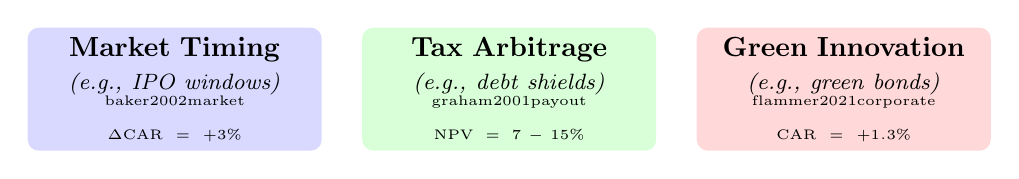
\begin{tikzpicture}[node distance=0.5cm]
		\node (strat1) [rounded corners,fill=blue!15,text width=3.5cm,align=center] {\textbf{Market Timing} \\ {\footnotesize\textit{(e.g., IPO windows)}} \\ \tiny\textcite{baker2002market}  \\ {\tiny $\Delta \text{CAR} = +3\%$}};
		\node (strat2) [right=of strat1,rounded corners,fill=green!15,text width=3.5cm,align=center] {\textbf{Tax Arbitrage} \\ {\footnotesize\textit{(e.g., debt shields)}} \\ \tiny\textcite{graham2001payout} \\ {\tiny $\text{NPV} = 7-15\%$}};
		\node (strat3) [right=of strat2,rounded corners,fill=red!15,text width=3.5cm,align=center] {\textbf{Green Innovation} \\ {\footnotesize\textit{(e.g., green bonds)}} \\ \tiny\textcite{flammer2021corporate} \\ {\tiny $\text{CAR} = +1.3\%$}};
	\end{tikzpicture}
	\vspace{0.5cm}
	\begin{itemize}
		\item \textcolor{blue}{Short-Term}: 1–3 years (volatility-driven)
		\item \textcolor{green}{Medium-Term}: 5–10 years (structural)
		\item \textcolor{red}{Long-Term}: 10+ years (innovation-driven)
	\end{itemize}
\end{frame}

\begin{frame}{Creating Value through Market Timing: Can Firms Fool Investors?}
	\begin{itemize}
		\item Theory: Firms might create value by \textit{fooling investors} through financing tactics.
		\item Reality: Sustained deception is difficult in reasonably efficient markets.
		\begin{itemize}
			\item Over time, asset prices converge to intrinsic values.
		\end{itemize}
		\item Risks of attempting to fool investors:
		\begin{itemize}
			\item Legal sanctions
			\item Reputation loss
			\item Market corrections that reverse any gains
		\end{itemize}
		\item Common examples:
		\begin{itemize}
			\item Earnings management and aggressive accounting
			\item Insider trading
			\item Market price manipulation
		\end{itemize}
	\end{itemize}
\end{frame}

\begin{frame}{Why Market Timing Fails: The Enron Case }
	\begin{columns}
		\column{0.6\textwidth}
		\textbf{Mechanics of Collapse\parencite{healy2003fall}}:
		\begin{itemize}
			\item Hidden debt via SPEs: \$1.2B off-balance-sheet
			\item Stock price drop: \$90.75 (2000) → \$0.26 (2001)
		\end{itemize}
		\column{0.4\textwidth}
		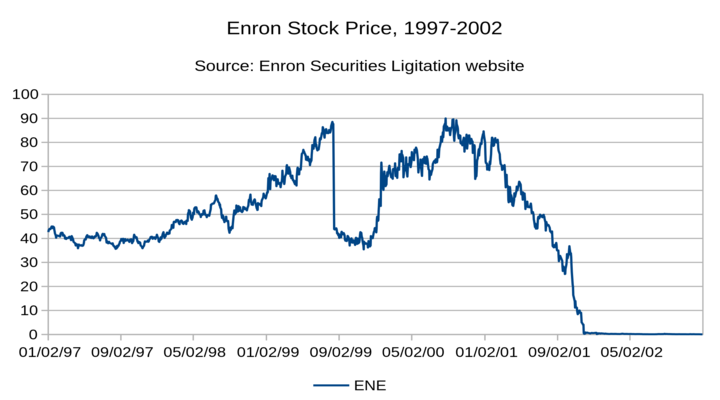
\includegraphics[width=\textwidth]{images/section1/enron_stock_chart.png}
	\end{columns}
	\vspace{0.3cm}
	\begin{alertblock}{Modern Enforcement \parencite{palantir2023}}
		AI tools (e.g., Palantir) detect anomalies in real-time. \\
		{\footnotesize\textcolor{gray}{Source: SEC 2023 Enforcement Report}}
	\end{alertblock}
\end{frame}

\begin{frame}{Reducing Costs or Increasing Subsidies: A Financing Channel}
	Certain financing structures offer explicit or implicit subsidies.
	\begin{block}{Illustration: Subsidized Bond Issuance}
		Ant Sports Co. applies for a tax-exempt, 5-year, \textyen 2 million industrial bond in Fujian to avoid relocating production to Vietnam.
		\begin{itemize}
			\item Regular debt cost: 10\%
			\item Industrial bond coupon: 5\%
			\item Annual interest savings: \textyen 100,000
		\end{itemize}
		\textbf{Question}: What is the NPV of accepting the subsidy?
	\end{block}
\end{frame}

\begin{frame}{Valuation of Subsidized Financing}
	\textbf{NPV Calculation}:
	\begin{align*}
		NPV &= \text{\textyen} 2,000,000 - \sum_{t=1}^5 \frac{\text{\textyen} 100,000}{1.1^t} - \frac{\text{\textyen} 2,000,000}{1.1^5} \\
		&= \text{\textyen} 2,000,000 - \text{\textyen} 1,620,921 \\
		&= \text{\textyen} 379,079
	\end{align*}
	\textbf{Conclusion}:  
	Ant Sports captures a \textbf{subsidy} worth \textyen 379,079 by issuing the industrial bond.

 \textbf{Interpretation}: The Fujian government provides an implicit subsidy equal to NPV via below-market rates
\end{frame}

\begin{frame}{Creating Value through Financial Innovation}
	\begin{block}{Core Idea}
		\textbf{Firms can create value by issuing new types of securities} that satisfy previously unmet investor preferences or risk-return demands.
	\end{block}
	
	\vspace{0.3cm}
	
	\begin{exampleblock}{Example: Convertible Bonds}
		\begin{itemize}
			\item \textbf{Downside protection}: Bond features limit investor losses.
			\item \textbf{Upside participation}: Embedded call option captures stock price appreciation.
			\item \textbf{Issuer benefits}: Lower financing costs and deferred equity dilution.
		\end{itemize}
	\end{exampleblock}
	
	\vspace{0.3cm}
	\begin{alertblock}{Important Caveat}
		The initial advantage often erodes quickly as competitors imitate the innovation, eliminating excess returns.
	\end{alertblock}
\end{frame}


\begin{frame}{Synthesis: Value Creation Pathways}
\begin{table}[h]
    \centering
    \resizebox{\textwidth}{!}{
	\begin{tabular}{lccp{6cm}}
		\toprule
		\textbf{Strategy} & \textbf{Persistence} & \textbf{Value Impact} & \textbf{Critical Considerations} \\
		\midrule
		Market Timing & Short-term & Low & Relies on transient mispricing; exposes firms to regulatory and reputational risks. \\
		Tax Optimization & Long-term & Medium & Requires durable alignment with legal structures and economic substance. \\
		Security Design & Medium-term & High & Demands continual adaptation to evolving investor needs and competitive imitation. \\
		\bottomrule
	\end{tabular}
    }
\end{table}

\begin{block}{Key Insights}
\begin{itemize}
	\item \textcolor{blue}{\textbf{Sustainable value}} arises from \textit{structural advantages}, not opportunistic tactics.
	\item \textcolor{green}{\textbf{Strategic imperative}}: Integrate financial engineering with superior operational execution.
\end{itemize}
\end{block}
\end{frame}


% \section[CS: Basic]{Capital Structure: Basic Concepts}
% \subsection{The Capital Structure Question and the Pie Theory}
\begin{frame}{Capital Structure and the Pie Theory}
	
	\begin{block}{Firm Value Identity}
		The total value of the firm is the sum of its debt and equity:
		\begin{equation}
			V = B + S
		\end{equation}
	\end{block}
	
	\vspace{-0.3cm}
	\begin{columns}[T]
		\column{0.7\textwidth}
		\textbf{Key Question:}  
		\begin{itemize}
			\item Can the firm change its value by adjusting the mix between debt and equity?
			\item If so, what is the optimal capital structure that maximizes firm value?
			\item This is the \textbf{Capital Structure Question}.
		\end{itemize}
		
		\column{0.3\textwidth}
		\begin{figure}
			\centering
			
\includegraphics[width=0.6\linewidth]{images/section2/firmvalue}
			\caption*{\tiny Capital structure changes the “slices” -- but does it grow the pie?}
		\end{figure}
	\end{columns}
	
	\vspace{-0.3cm}
	\begin{alertblock}{Objective}
		Choose the debt–equity ratio that \textbf{maximizes the total firm value}.
	\end{alertblock}
	
\end{frame}

\begin{frame}{Stockholders and Capital Structure Decisions}
	
	\textbf{Two Key Questions in Capital Structure:}
	\begin{enumerate}
		\item Why should shareholders care about \textit{maximizing firm value}, rather than just \textit{their own claims}?
		\item What debt–equity ratio maximizes shareholder wealth?
	\end{enumerate}
	
	\vspace{0.5cm}
	\begin{itemize}
		\item A change in capital structure affects the allocation between debt and equity.
		\item But it benefits shareholders \textbf{only if it increases total firm value}.
	\end{itemize}
	
	\vspace{0.3cm}
	\begin{alertblock}{Implication}
		Capital structure is irrelevant to shareholders unless it expands the overall size of the pie.
	\end{alertblock}
	
\end{frame}

\subsection{Financial Leverage and Firm Value: An Example}
\begin{frame}{Leverage Recapitalization: Setup}
	
	\textbf{Trans Am Corporation is currently unlevered.}  
	It is considering issuing \$4,000 of debt to repurchase equity.
	
	\begin{table}[h]
		\centering
		\resizebox{0.9\linewidth}{!}{
			\begin{tabular}{@{}lrr@{}}
				\toprule
				& \textbf{Unlevered} & \textbf{Levered (Proposed)} \\ \midrule
				Total Assets              & \$8,000            & \$8,000                      \\
				Debt                      & \$0                & \$4,000                      \\
				Equity                    & \$8,000            & \$4,000                      \\
				Interest Rate             & 10\%               & 10\%                         \\
				Market Price per Share    & \$20               & \$20                         \\
				Shares Outstanding        & 400                & 200                          \\
				\bottomrule
			\end{tabular}
		}
	\end{table}
	

	\begin{alertblock}{Key Question}
		How does leverage affect EPS and ROE under different operating scenarios?
	\end{alertblock}
\end{frame}

\begin{frame}{EPS and ROE Under Different Scenarios}
	
	\textbf{Unlevered Structure (All-Equity)}
	\begin{table}
		\centering
		\resizebox{0.6\linewidth}{!}{
		\begin{tabular}{@{}lccc@{}}
			\toprule
			& Recession & Expected & Expansion \\ \midrule
			Earnings      & \$400     & \$1,200  & \$2,000   \\
			ROE           & 5\%       & 15\%     & 25\%      \\
			EPS           & \$1       & \$3      & \$5       \\ \bottomrule
		\end{tabular}
	}
	\end{table}
	
	\textbf{Leveraged Structure (Debt = \$4,000)}
	\begin{table}
		\centering
		\resizebox{0.6\linewidth}{!}{
		\begin{tabular}{@{}lccc@{}}
			\toprule
			& Recession & Expected & Expansion \\ \midrule
			EBIT                  & \$400     & \$1,200  & \$2,000   \\
			Interest Expense      & \$400     & \$400    & \$400     \\
			Earnings After Interest & \$0     & \$800    & \$1,600   \\
			ROE                   & 0\%       & 20\%     & 40\%      \\
			EPS                   & \$0       & \$4      & \$8       \\ \bottomrule
		\end{tabular}
	}
	\end{table}
	
	\begin{block}{Observation}
		Leverage increases return sensitivity -- it amplifies both gains and losses.
	\end{block}
	
\end{frame}

\begin{frame}{EPS as a Function of EBIT (Leveraged vs. Unleveraged)}
	
	\begin{figure}
		\centering
		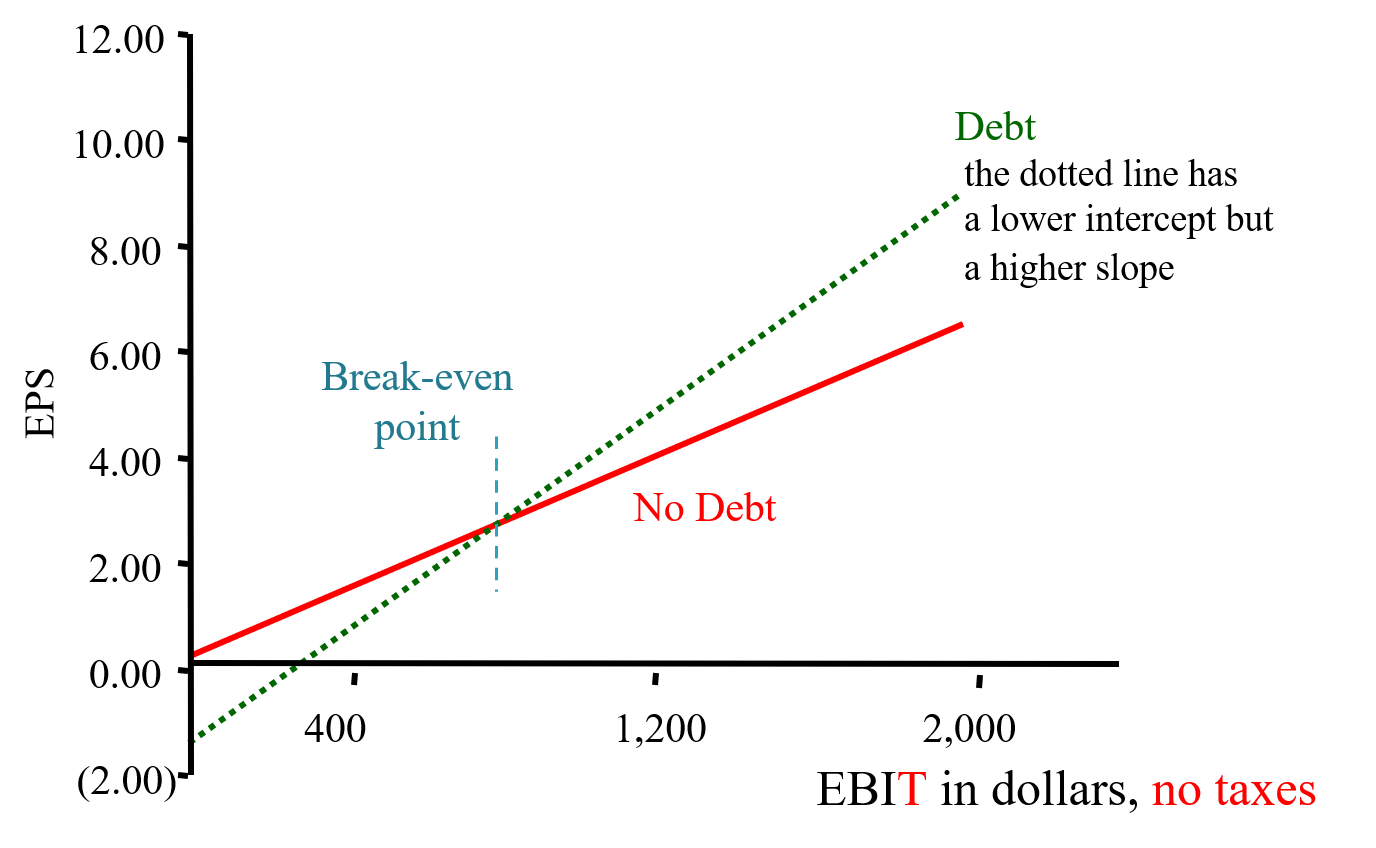
\includegraphics[width=0.6\linewidth]{images/section2/epschanges.png}
	\end{figure}
	
	\vspace{0.3cm}
	\begin{block}{Interpretation}
		The break-even EBIT is where both structures yield the same EPS.  
		Beyond that point, leverage boosts EPS; below it, leverage hurts.
	\end{block}
\end{frame}

\begin{frame}{Break-Even EBIT: When Does Leverage Help?}
	
	\begin{itemize}
		\item Financial leverage increases EPS only when EBIT exceeds a certain threshold -- the \textbf{break-even EBIT}.
		\item Below that point, interest expense outweighs the benefit of fewer shares outstanding.
	\end{itemize}
	
	\begin{block}{Example Setup}
		MPD Corporation plans to shift from an all-equity structure to a leveraged one by issuing \$1 million of debt at 9\% interest to repurchase shares.  
		\vspace{1mm}
		
		Currently:  
		\begin{itemize}
			\item 200,000 shares at \$20/share  
			\item No debt  
		\end{itemize}
		
		\textbf{Question:}  
		What is the minimum EBIT that would make the restructuring EPS-neutral (i.e., the break-even point)?
	\end{block}
	
\end{frame}

\begin{frame}{Break-Even EBIT: Step-by-Step Calculation}
	\small
	\textbf{Unlevered EPS (original):}
	\[
	\text{EPS}_\text{Old} = \frac{\text{EBIT}}{200{,}000}
	\]
	
	\textbf{Leveraged EPS (new):}
	\begin{itemize}
		\item Interest expense = \$1,000,000 × 9\% = \$90,000
		\item Shares repurchased = \$1,000,000 / \$20 = 50,000
		\item Shares outstanding after repurchase = 150,000
		\[
		\text{EPS}_\text{New} = \frac{\text{EBIT} - 90{,}000}{150{,}000}
		\]
	\end{itemize}
	

	\textbf{Set equal:}
	\begin{align*}
		\frac{\text{EBIT}}{200{,}000} = \frac{\text{EBIT} - 90{,}000}{150{,}000} 
		\Rightarrow \text{EBIT} = \$360{,}000
	\end{align*}
	\vspace{-0.4cm}
	\begin{alertblock}{Result}
		EBIT must exceed \$360,000 for leverage to increase EPS.
	\end{alertblock}
	
\end{frame}

\begin{frame}{Interpreting Break-Even EBIT}
	
	\begin{itemize}
		\item \textbf{Definition:}  
		Break-even EBIT is the level at which EPS under two capital structures (leveraged and unleveraged) is equal.
		
		\item \textbf{If EBIT > Break-even:}  
		\begin{itemize}
			\item Leverage amplifies returns (higher EPS)
			\item Financial structure becomes \textbf{advantageous}
		\end{itemize}
		
		\item \textbf{If EBIT < Break-even:}  
		\begin{itemize}
			\item Interest costs drag down earnings
			\item Leverage is \textbf{detrimental} -- equity returns shrink, risk of distress rises
		\end{itemize}
		
		\item \textbf{Managerial Use:}  
		Helps determine when adding leverage is expected to create or destroy shareholder value
	\end{itemize}
	
	\begin{block}{Teaching Insight}
		Break-even EBIT offers a bridge between capital structure theory and real-world decision-making.
	\end{block}
	
\end{frame}

\begin{frame}{Homemade Leverage: Core Insights}
	
	\begin{itemize}
		\item \textbf{Key Idea:}  
		Investors can replicate the effects of corporate leverage by borrowing on their own account.
		
		\item \textbf{Implications from Example:}
		\begin{itemize}
			\item At high EBIT levels, leverage magnifies shareholder returns (EPS, ROE $\uparrow$).
			\item At low EBIT levels, fixed interest costs amplify downside risk (EPS, ROE $\downarrow$).
			\item Financial leverage increases the volatility of shareholder outcomes.
			\item Because investors can replicate leverage on their own, capital structure may be irrelevant -- under ideal conditions.
		\end{itemize}
	\end{itemize}
	
	\vspace{0.2cm}
	\begin{alertblock}{Takeaway}
		The value of the firm should not depend on how it's financed -- if investors can create “homemade leverage.”
	\end{alertblock}
	
\end{frame}

\begin{frame}{Comparing Corporate and Homemade Leverage}
	\vspace{-0.2cm}
	\begin{table}[h]
		\centering
		\resizebox{0.9\linewidth}{!}{
			\begin{tabular}{@{}lccc@{}}
				\toprule
				\textbf{Scenario} & \textbf{Recession} & \textbf{Expected} & \textbf{Expansion} \\
				\midrule
				\multicolumn{4}{l}{\textit{Strategy A: 100 Shares of Levered Equity}} \\
				EPS (Levered)     & 0    & \$4   & \$8   \\
				Total Earnings    & 0    & \$400 & \$800 \\
				Initial Investment & \multicolumn{3}{r}{100 × \$20 = \$2,000} \\
				\midrule
				\multicolumn{4}{l}{\textit{Strategy B: Homemade Leverage (200 Unlevered – \$2,000 borrowed)}} \\
				EPS (Unlevered)   & \$1   & \$3   & \$5   \\
				Total Earnings    & \$200 & \$600 & \$1,000 \\
				Interest Expense  & \$200 & \$200 & \$200 \\
				Net Earnings      & 0     & \$400 & \$800 \\
				Initial Investment & \multicolumn{3}{r}{200 × \$20 – \$2,000 = \$2,000} \\
				\bottomrule
			\end{tabular}
		}
	\end{table}
	
	\begin{block}{Conclusion}
		Investor-created leverage perfectly replicates corporate leverage -- under ideal conditions.
	\end{block}
	
\end{frame}

\begin{frame}{What Does Homemade Leverage Teach Us?}
	
	\begin{itemize}
		\item \textbf{If} investors can borrow and lend at the same rate as firms,  
		\item \textbf{And if} there are no taxes, transaction costs, or bankruptcy costs,
	\end{itemize}
	
	\vspace{0.3cm}
	\begin{block}{Then...}
		Capital structure becomes irrelevant:  
		\[
		\text{Firm Value (V)} \quad \text{is the same whether it’s financed by debt or equity.}
		\]
	\end{block}
	
	\vspace{0.2cm}
	\begin{itemize}
		\item Investors can always adjust leverage themselves.
		\item This logic forms the foundation of the \textbf{Modigliani–Miller Proposition I}.
	\end{itemize}
\end{frame}

\subsection{Modigliani–Miller Model}
\begin{frame}{Capital Structure: Does It Matter?}
	
	\begin{itemize}
		\item In 1958, \textcite{modigliani1958cost} proposed a revolutionary theory of capital structure.  
		\item Their core question: \textbf{Can financing choices affect firm value?}
		\item The M\&M model provides a framework to explore when capital structure is irrelevant -- and when it matters.
	\end{itemize}
	
	
	\vspace{0.2cm}
	\begin{alertblock}{What Comes Next}
		We will analyze three progressively more realistic cases that relax ideal assumptions.
	\end{alertblock}
	
\end{frame}

\begin{frame}{Three Cases in M\&M Capital Structure Theory}
	
	\begin{itemize}
		\item \textbf{Case I: Perfect Capital Markets}
		\begin{itemize}
			\item No taxes, no transaction costs, no bankruptcy
			\item Capital structure is irrelevant
		\end{itemize}
		
		\item \textbf{Case II: Corporate Taxes Introduced}
		\begin{itemize}
			\item Interest is tax-deductible $\rightarrow$ Debt creates value
			\item Incentive to fully lever up
		\end{itemize}
		
		\item \textbf{Case III: Taxes + Financial Distress}
		\begin{itemize}
			\item Trade-off between tax shield and bankruptcy risk
			\item Optimal capital structure balances both
		\end{itemize}
	\end{itemize}
	
	\vspace{0.2cm}
	\begin{block}{Literature Evolution}
		These cases laid the foundation for the \textit{trade-off theory} of capital structure.  
		See also: \textcite{miller1988nobel}
	\end{block}
	
\end{frame}
\begin{frame}{Key Assumptions Behind the M\&M Model}
	
	\textbf{To understand why capital structure may be irrelevant, we must first understand the model’s ideal conditions:}
	
	\vspace{0.3cm}
	\begin{itemize}
		\item \textbf{Perfect Capital Markets}
		\begin{itemize}
			\item No taxes or transaction costs
			\item Firms and investors borrow/lend at the same rate
			\item No asymmetric information
		\end{itemize}
		
		\item \textbf{Homogeneous Expectations}
		\begin{itemize}
			\item All investors agree on firm cash flows and risk
		\end{itemize}
		
		\item \textbf{Same Risk Class}
		\begin{itemize}
			\item Firms compared must have similar business risk
		\end{itemize}
	\end{itemize}
	
	\vspace{0.2cm}
	\begin{alertblock}{Next}
		We now turn to Case I -- where capital structure does not affect firm value.
	\end{alertblock}
	
\end{frame}

\subsubsection{Case I}
\begin{frame}{MM Proposition I (No Taxes): Value Irrelevance}
	
	\begin{block}{M\&M Proposition I}
		Under perfect capital markets and no taxes:
		\[
		V_L = V_U
		\]
		\textit{The value of a levered firm equals that of an unlevered firm.}
	\end{block}
	
	\begin{itemize}
		\item Firm value is determined solely by the cash flows and risk of its assets.
		\item Capital structure does not create or destroy value -- it’s just slicing the same pie differently.
		\item Investors can replicate any capital structure through homemade leverage.
	\end{itemize}
	
	\vspace{0.2cm}
	\tiny{\textcite{modigliani1958cost}}
\end{frame}

\begin{frame}{MM Proposition II (No Taxes): Cost of Equity}
	
	\begin{block}{M\&M Proposition II}
		As leverage increases, equity becomes riskier:
		\[
		R_S = R_0 + \frac{B}{S}(R_0 - R_B)
		\]
	\end{block}
	
	\begin{itemize}
		\item \(R_S\): Cost of equity  
		\item \(R_0\): Cost of capital for the unlevered firm (business risk)  
		\item \(R_B\): Cost of debt  
	\end{itemize}
	\begin{exampleblock}{Key Insight:}
		Equity holders demand higher returns as financial leverage increases risk.
	\end{exampleblock}
	
\end{frame}

\begin{frame}{MM Proposition II: Derivation}
	
	\textbf{Start with WACC:}
	\[
	R_0 = \frac{B}{B+S} R_B + \frac{S}{B+S} R_S
	\]
	
	\vspace{0.3cm}
	\textbf{Multiply both sides by } \(\frac{B+S}{S}\):
	
	\[
	\frac{B}{S} R_B + R_S = \frac{B+S}{S} R_0
	\]
	
	\vspace{0.3cm}
	\textbf{Solve for } \(R_S\):
	
	\[
	R_S = R_0 + \frac{B}{S}(R_0 - R_B)
	\]
	
	\begin{block}{Conclusion}
		Equity return increases linearly with the debt-equity ratio.
	\end{block}
	
\end{frame}

\begin{frame}{Visualizing Leverage and the Cost of Capital}
	\vspace{-0.5cm}
	\begin{figure}
		\centering
		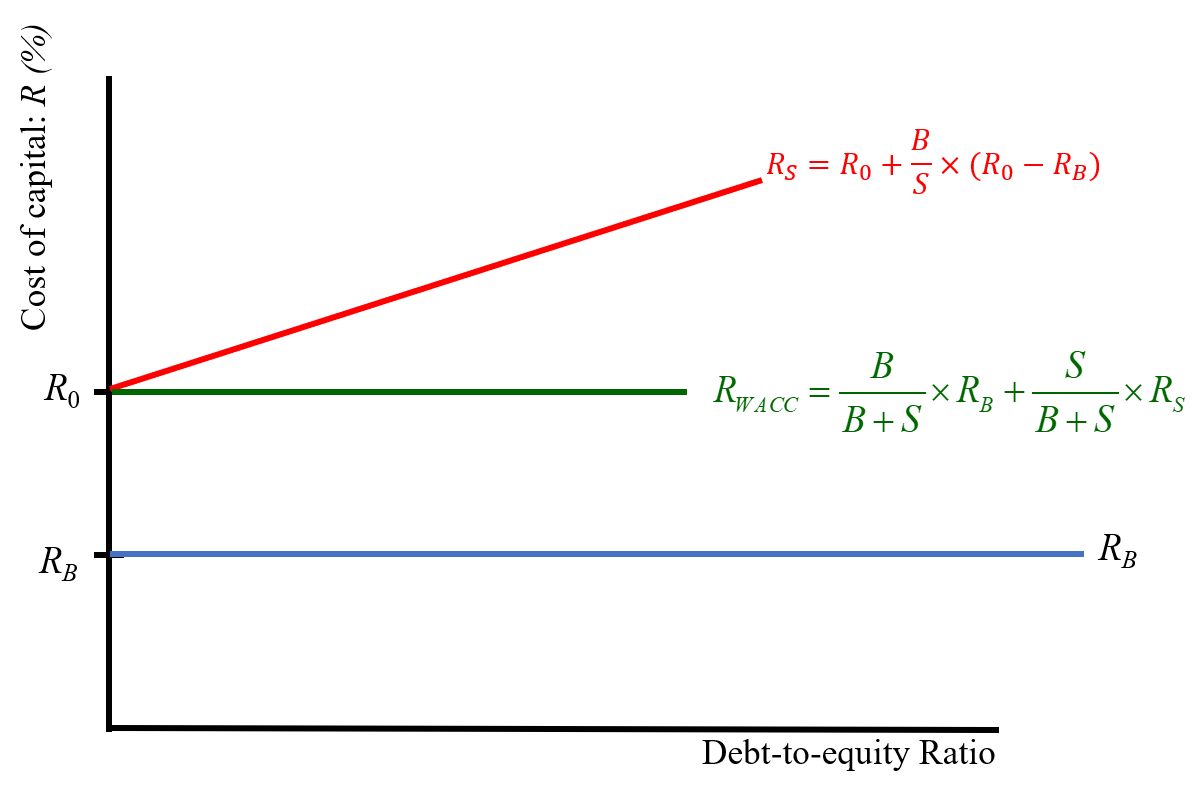
\includegraphics[width=0.7\textwidth]{images/section2/wacc.png}
	\end{figure}
	\vspace{-0.5cm}
	\begin{block}{Interpretation}
		\begin{itemize}
			\item \(R_S\) increases with leverage due to higher risk.
			\item \(WACC = R_0\) remains constant -- consistent with M\&M Proposition I.
		\end{itemize}
	\end{block}

\end{frame}

\begin{frame}{Business Risk vs. Financial Risk}
	
	\textbf{According to M\&M Proposition II:}
	
	\begin{itemize}
		\item The cost of equity includes:
		\begin{enumerate}
			\item \textbf{Business Risk} -- driven by operations and assets.
			\item \textbf{Financial Risk} -- introduced by the use of leverage.
		\end{enumerate}
		
		\item \(R_S = R_0 + \frac{B}{S}(R_0 - R_B)\)
		\begin{itemize}
			\item \(R_0\): captures business risk
			\item \(\frac{B}{S}(R_0 - R_B)\): captures financial risk
		\end{itemize}
		
		\item Leverage does not affect business risk -- only financial risk.
	\end{itemize}
	
	\vspace{0.2cm}
	\begin{alertblock}{Conclusion}
		More leverage $\rightarrow$ more financial risk $\rightarrow$ higher required return on equity.
	\end{alertblock}
	
\end{frame}


\section{Capital Structure: Limits to the Use of Debt}
\begin{frame}{Capital Structure: What Limits the Use of Debt?}
	\small
	\textbf{Beyond Tax Shields — Why Don't Firms Use 100\% Debt?}
	\small
	In this section, we explore factors that challenge the simple tax-based view of optimal capital structure:
	\vspace{-3mm}
	
	\begin{itemize}
		\item \textbf{Case III: Trade-Off Theory}  
		Firms weigh the tax benefits of debt against the costs of financial distress.
		
		\item \textbf{Signaling Effects}  
		Capital structure choices can signal private information to investors.
		\item \textbf{Agency Costs of Equity}  
		Equity financing may create incentive misalignments between owners and managers.
		
		\item \textbf{Pecking Order Theory}  
		Firms prefer internal funds, then debt, and issue equity only as a last resort.
		
		\item \textbf{Real-World Constraints}  
		Legal, institutional, and industry-specific frictions matter too.
	\end{itemize}
	\vspace{-3mm}
	\begin{alertblock}{Goal of This Section}
		To understand why real-world firms often choose \textbf{moderate} debt levels — not extremes.
	\end{alertblock}
	
\end{frame}

\subsection{Costs of Financial Distress}
\begin{frame}{The Downside of Debt: Financial Distress}
	
	\begin{itemize}
		\item Debt creates tax benefits — but also introduces fixed obligations.
		\item \textbf{Failure to meet interest or principal payments leads to distress.}
		\item Ultimate form of distress: \textbf{Bankruptcy}
		\begin{itemize}
			\item Control of assets transfers from shareholders to creditors.
		\end{itemize}
		\item In the real world, \textbf{costs of distress may offset the benefits of debt}.
	\end{itemize}
	
	\vspace{0.2cm}
	\begin{alertblock}{Core Idea}
		There is a trade-off between tax shields and financial distress costs.
	\end{alertblock}
	
\end{frame}

\begin{frame}{Illustration: Bankruptcy Pressure}
	
	\textbf{Cash Flow Uncertainty:}
	
	\begin{itemize}
		\item EBIT = \$100 (Boom) or \$50 (Recession), each with 50\% probability.
		\item Knight Corp: debt requires \$49 in payments.
		\item Day Corp: debt requires \$60 in payments.
	\end{itemize}
	
	\vspace{0.2cm}
	\begin{table}
		\centering
		\caption*{\textbf{Cash Flow Distribution (No Legal Fees)}}
		\begin{tabular}{@{}lcccc@{}}
			\toprule
			& \multicolumn{2}{c}{\textit{Knight Corp}} & \multicolumn{2}{c}{\textit{Day Corp}} \\
			& Boom & Recession & Boom & Recession \\ \midrule
			Firm Cash Flow & \$100 & \$50 & \$100 & \$50 \\
			To Bondholders & \$49 & \$49 & \$60 & \$50 \\
			To Shareholders & \$51 & \$1 & \$40 & \$0 \\ \bottomrule
		\end{tabular}
	\end{table}
	
	\vspace{0.2cm}
	\textbf{Observation:}  
	Day Corp’s higher leverage reduces shareholder value and increases distress risk.
\end{frame}

\begin{frame}{Realistic Scenario: Legal Costs of Distress}
	
	\textbf{In Distress, Lawyers Get Paid First}
	
	\begin{itemize}
		\item Legal battles reduce available cash flow — even before creditors are paid.
		\item Suppose bankruptcy/legal fees = \$15 in recession scenario.
	\end{itemize}
	
	\vspace{0.2cm}
	\begin{table}
		\centering
		\caption*{\textbf{Day Corp with Legal Costs}}
		\begin{tabular}{@{}lcc@{}}
			\toprule
			& Boom & Recession \\ \midrule
			Cash Flow & \$100 & \$50 \\
			To Bondholders & \$60 & \$35 \\
			To Shareholders & \$40 & \$0 \\ \bottomrule
		\end{tabular}
	\end{table}
	
	\vspace{0.2cm}
	\textbf{Conclusion:}  
	Distress reduces total value available to claimholders — debt becomes costly.
\end{frame}

\begin{frame}{Direct Costs of Financial Distress}
	
	\textbf{Legal and Administrative Costs:}
	\begin{itemize}
		\item Legal fees during reorganization or liquidation can be substantial.
		\item Enron: \$1 billion; WorldCom: \$600 million
		\item These costs are paid before creditors or shareholders receive anything.
	\end{itemize}
	
	\vspace{0.3cm}
	\textbf{Empirical Estimates:}
	\begin{itemize}
		\item \textcite{white1980bankruptcy}: Direct costs $\approx$ 3\% of firm value
		\item \textcite{warner1977bankruptcy}: Average $\approx$ 1\% of firm value (7 years before bankruptcy)
	\end{itemize}
	
	\vspace{0.3cm}
	\begin{alertblock}{Key Point}
		Even small percentage costs can erode tax benefits when distress probability is high.
	\end{alertblock}
	
\end{frame}

\begin{frame}{Indirect Costs of Financial Distress}
	
	\textbf{Harder to Observe — Still Very Real:}
	\begin{itemize}
		\item Loss of customers or suppliers
		\item Difficulty attracting or retaining talent
		\item Strategic delays or loss of growth opportunities
	\end{itemize}
	
	\vspace{0.3cm}
	\textbf{Example: GM \& Chrysler (2008)}
	\begin{itemize}
		\item 75\% of surveyed consumers said they wouldn’t buy from a bankrupt carmaker.
		\item Financial distress amplified by loss of confidence.
	\end{itemize}
	
	\vspace{0.3cm}
	\textbf{Key Feature:}  
	Difficult to measure — but can far exceed direct costs.
	
\end{frame}

\subsubsection{Agency Costs: Equity vs. Debt Conflict}
\begin{frame}{Agency Costs: Equity vs. Debt Conflict}
	
	\textbf{When a firm issues debt, the interests of stockholders and bondholders diverge.}
	
	\begin{itemize}
		\item Equityholders may pursue \textbf{self-serving strategies} that shift value from creditors.
		\item These strategies increase the risk of default, reduce firm value, and are especially problematic near distress.
		\item The resulting value loss is known as an \textbf{agency cost of debt}.
	\end{itemize}
	
	\vspace{0.3cm}
	\begin{block}{Three Common Selfish Strategies}
		\begin{enumerate}
			\item Excessive risk-taking (gamble for resurrection)
			\item Underinvestment (debt overhang)
			\item Asset stripping or “milking the property”
		\end{enumerate}
	\end{block}
	
\end{frame}

\begin{frame}{Case: Company in Financial Distress}
	
	\textbf{Balance Sheet of a Distressed Firm}
	
	\begin{table}
		\centering
		\begin{tabular}{@{}llllll@{}}
			\toprule
			Assets      & BV    & MV    & Liabilities & BV    & MV    \\ \midrule
			Cash        & \$200 & \$200 & Bonds       & \$300 & \$200 \\
			Fixed Assets & \$400 & \$0   & Equity      & \$300 & \$0   \\
			Total       & \$600 & \$200 & Total       & \$600 & \$200 \\ \bottomrule
		\end{tabular}
	\end{table}
	
	\begin{itemize}
		\item Liquidation today: Bondholders receive all \$200 → Shareholders get \textbf{nothing}.
		\item But shareholders control investment decisions.
	\end{itemize}
	
\end{frame}

\begin{frame}{Selfish Strategy 1: Excessive Risk-Taking}
	
	\textbf{The Gamble: Use all \$200 cash for a risky investment}
	
	\begin{table}
		\centering
		\begin{tabular}{lll}
			\toprule
			Outcome     & Probability & Payoff \\ \midrule
			Win Big     & 10\%        & \$1,000 \\
			Lose All    & 90\%        & \$0 \\ \bottomrule
		\end{tabular}
	\end{table}
	
	\vspace{0.2cm}
	\begin{itemize}
		\item Required return = 50\%, investment cost = \$200
		\item Expected payoff = \$100 → NPV = \(-133\)
	\end{itemize}
	
	\vspace{0.2cm}
	\begin{equation*}
		\text{NPV} = -200 + \frac{100}{1.5} = -133
	\end{equation*}
	
	\begin{alertblock}{Insight}
		The firm destroys value, but equityholders benefit in the up-state.
	\end{alertblock}
	
\end{frame}

\begin{frame}{Value Shift from Bondholders to Stockholders}
	
	\begin{itemize}
		\item \textbf{Expected CF Distribution}:
		\begin{itemize}
			\item To Bondholders: \$30 → PV = \$20
			\item To Stockholders: \$70 → PV = \$47
		\end{itemize}
		
		\item \textbf{Compare to status quo:}
		\begin{itemize}
			\item PV of Bonds (no gamble) = \$200
			\item PV of Stock = \$0
		\end{itemize}
	\end{itemize}
	
	\begin{alertblock}{Conclusion}
		Equityholders shift value from bondholders → destroy firm value.
	\end{alertblock}
	
\end{frame}


\begin{frame}{Selfish Strategy 2: Underinvestment (Debt Overhang)}
	
	\begin{block}{The Problem}
		Equityholders refuse to invest in value-enhancing projects that mostly benefit bondholders.
	\end{block}
	
	\begin{itemize}
		\item Project: Cost = \$300 → PV = \$318.18
		\item Required capital = \$100 from shareholders
		\item Return to firm > cost, but return to shareholders is negative
	\end{itemize}
	
	\begin{equation*}
		\text{NPV} = -300 + \frac{350}{1.1} = 18.18 > 0
	\end{equation*}
	
\end{frame}

\begin{frame}{Underinvestment: Who Gets What?}
	
	\begin{itemize}
		\item \textbf{Payoffs:}
		\begin{itemize}
			\item Bondholders: \$300 → PV = \$272.73
			\item Shareholders: \$50 → PV = \$45.45
			\item But \$100 out-of-pocket → Net PV to shareholders = \textbf{-\$54.55}
		\end{itemize}
		
		\item \textbf{Result:} Shareholders rationally reject positive-NPV project.
		
	\end{itemize}
	
	\begin{alertblock}{Outcome}
		Project creates value for the firm — but not for shareholders.
	\end{alertblock}
	
\end{frame}

\begin{frame}{Selfish Strategy 3: Milking the Property}
	
	\textbf{Tactics to extract value before bankruptcy:}
	
	\begin{itemize}
		\item \textbf{Liquidating dividends:}
		\begin{itemize}
			\item Firm pays out \$200 dividend to shareholders
			\item Leaves bondholders with no recovery value
			\item Often violates bond covenants
		\end{itemize}
		
		\item \textbf{Excessive perquisites:}
		\begin{itemize}
			\item Use corporate resources for personal consumption
			\item Hard to monitor, especially in privately held firms
		\end{itemize}
	\end{itemize}
	
	\begin{alertblock}{Key Issue}
		Shareholders extract private benefits — even if firm enters default.
	\end{alertblock}
	
\end{frame}

\begin{frame}{Summary: Who Pays for Selfish Behavior?}
	
	\begin{itemize}
		\item These distortions arise primarily when:
		\begin{itemize}
			\item Firm is highly leveraged
			\item Distress or default is likely
		\end{itemize}
		
		\item \textbf{Bondholders react:}
		\begin{itemize}
			\item Raise required yield
			\item Demand covenants
		\end{itemize}
		
		\item \textbf{Stockholders ultimately pay:}
		\begin{itemize}
			\item Higher cost of debt reduces equity value
			\item Financing becomes expensive or inaccessible
		\end{itemize}
	\end{itemize}
	
	\vspace{0.3cm}
	\begin{alertblock}{Conclusion}
		Agency conflicts raise the effective cost of debt — and limit a firm’s ability to borrow.
	\end{alertblock}
	
\end{frame}

\subsubsection{Mitigating Agency Conflicts Between Shareholders and Creditors}
\begin{frame}{Mitigating Conflict: Protective Covenants}
	
	\textbf{Bond Covenants} are contractual restrictions designed to align stockholder and bondholder interests by reducing agency costs.
	
	\begin{block}{Types of Covenants}
		\begin{itemize}
			\item \textbf{Negative Covenants:} Prohibit risky actions
			\begin{itemize}
				\item No sale or lease of major assets without approval
				\item No issuance of additional long-term debt
			\end{itemize}
			
			\item \textbf{Positive Covenants:} Require prudent behavior
			\begin{itemize}
				\item Maintain minimum levels of working capital
				\item Provide regular financial statements
			\end{itemize}
		\end{itemize}
	\end{block}
	
	\vspace{0.2cm}
	\textbf{Tradeoff:}  
	Though they reduce financial flexibility, covenants can lower borrowing costs and increase firm value by protecting creditor claims.
	
\end{frame}
\begin{frame}{Mitigating Conflict: Debt Coordination and Hybrid Claims}
	
	\textbf{Debt Consolidation Reduces Conflict Among Creditors}
	
	\begin{itemize}
		\item Bankruptcy costs rise when multiple creditors compete for limited assets.
		\item Solution: Fewer, centralized creditors → Easier negotiation in distress.
		\item Example: One lead lender finances all long-term debt.
	\end{itemize}
	
	\vspace{0.3cm}
	\textbf{Blending Stakeholder Roles}
	
	\begin{itemize}
		\item Encourage \textbf{creditor equity ownership}: debt holders also hold shares
		\item Aligns incentives — both care about total firm value, not just claim-specific returns
		\item Common in restructurings, PE-backed LBOs, or convertible bond structures
	\end{itemize}
	
	\vspace{0.2cm}
	\begin{alertblock}{Goal}
		Reduce value-destroying conflicts by integrating or coordinating stakeholder interests.
	\end{alertblock}
	
\end{frame}

\begin{frame}{Looking Ahead: Broader Mechanism Design}
	
	While protective covenants and creditor coordination help reduce agency conflicts, modern corporate finance also utilizes other contractual tools:
	
	\begin{itemize}
		\item \textbf{Convertible Bonds}: align incentives by letting creditors participate in upside.
		\item \textbf{Performance-Based Covenants}: dynamically adjust restrictions based on financial ratios.
		\item \textbf{Equity Issuance}: may serve as a signal of management confidence — or distress.
	\end{itemize}
	
	\vspace{0.3cm}
	\begin{alertblock}{Next}
		These institutional designs help mitigate the costs of debt, but they do not eliminate them.  
		We now turn to the broader \textbf{Trade-Off Theory}, which balances benefits (like tax shields) with costs (like financial distress and agency).
	\end{alertblock}
	
\end{frame}

\subsection{Trade-Off Theory of Capital Structure}
\begin{frame}{The Static Trade-Off Theory}
	
	\begin{itemize}
		\item Firms trade off the benefits of debt (tax shields) against the costs of financial distress.
		\item \textbf{Static Trade-Off Theory:}  
		Borrowing continues until:
		\[
		\text{Marginal Tax Shield} = \text{Marginal Distress Cost}
		\]
	\end{itemize}
	\vspace{-3mm}
	\begin{figure}
		\centering
		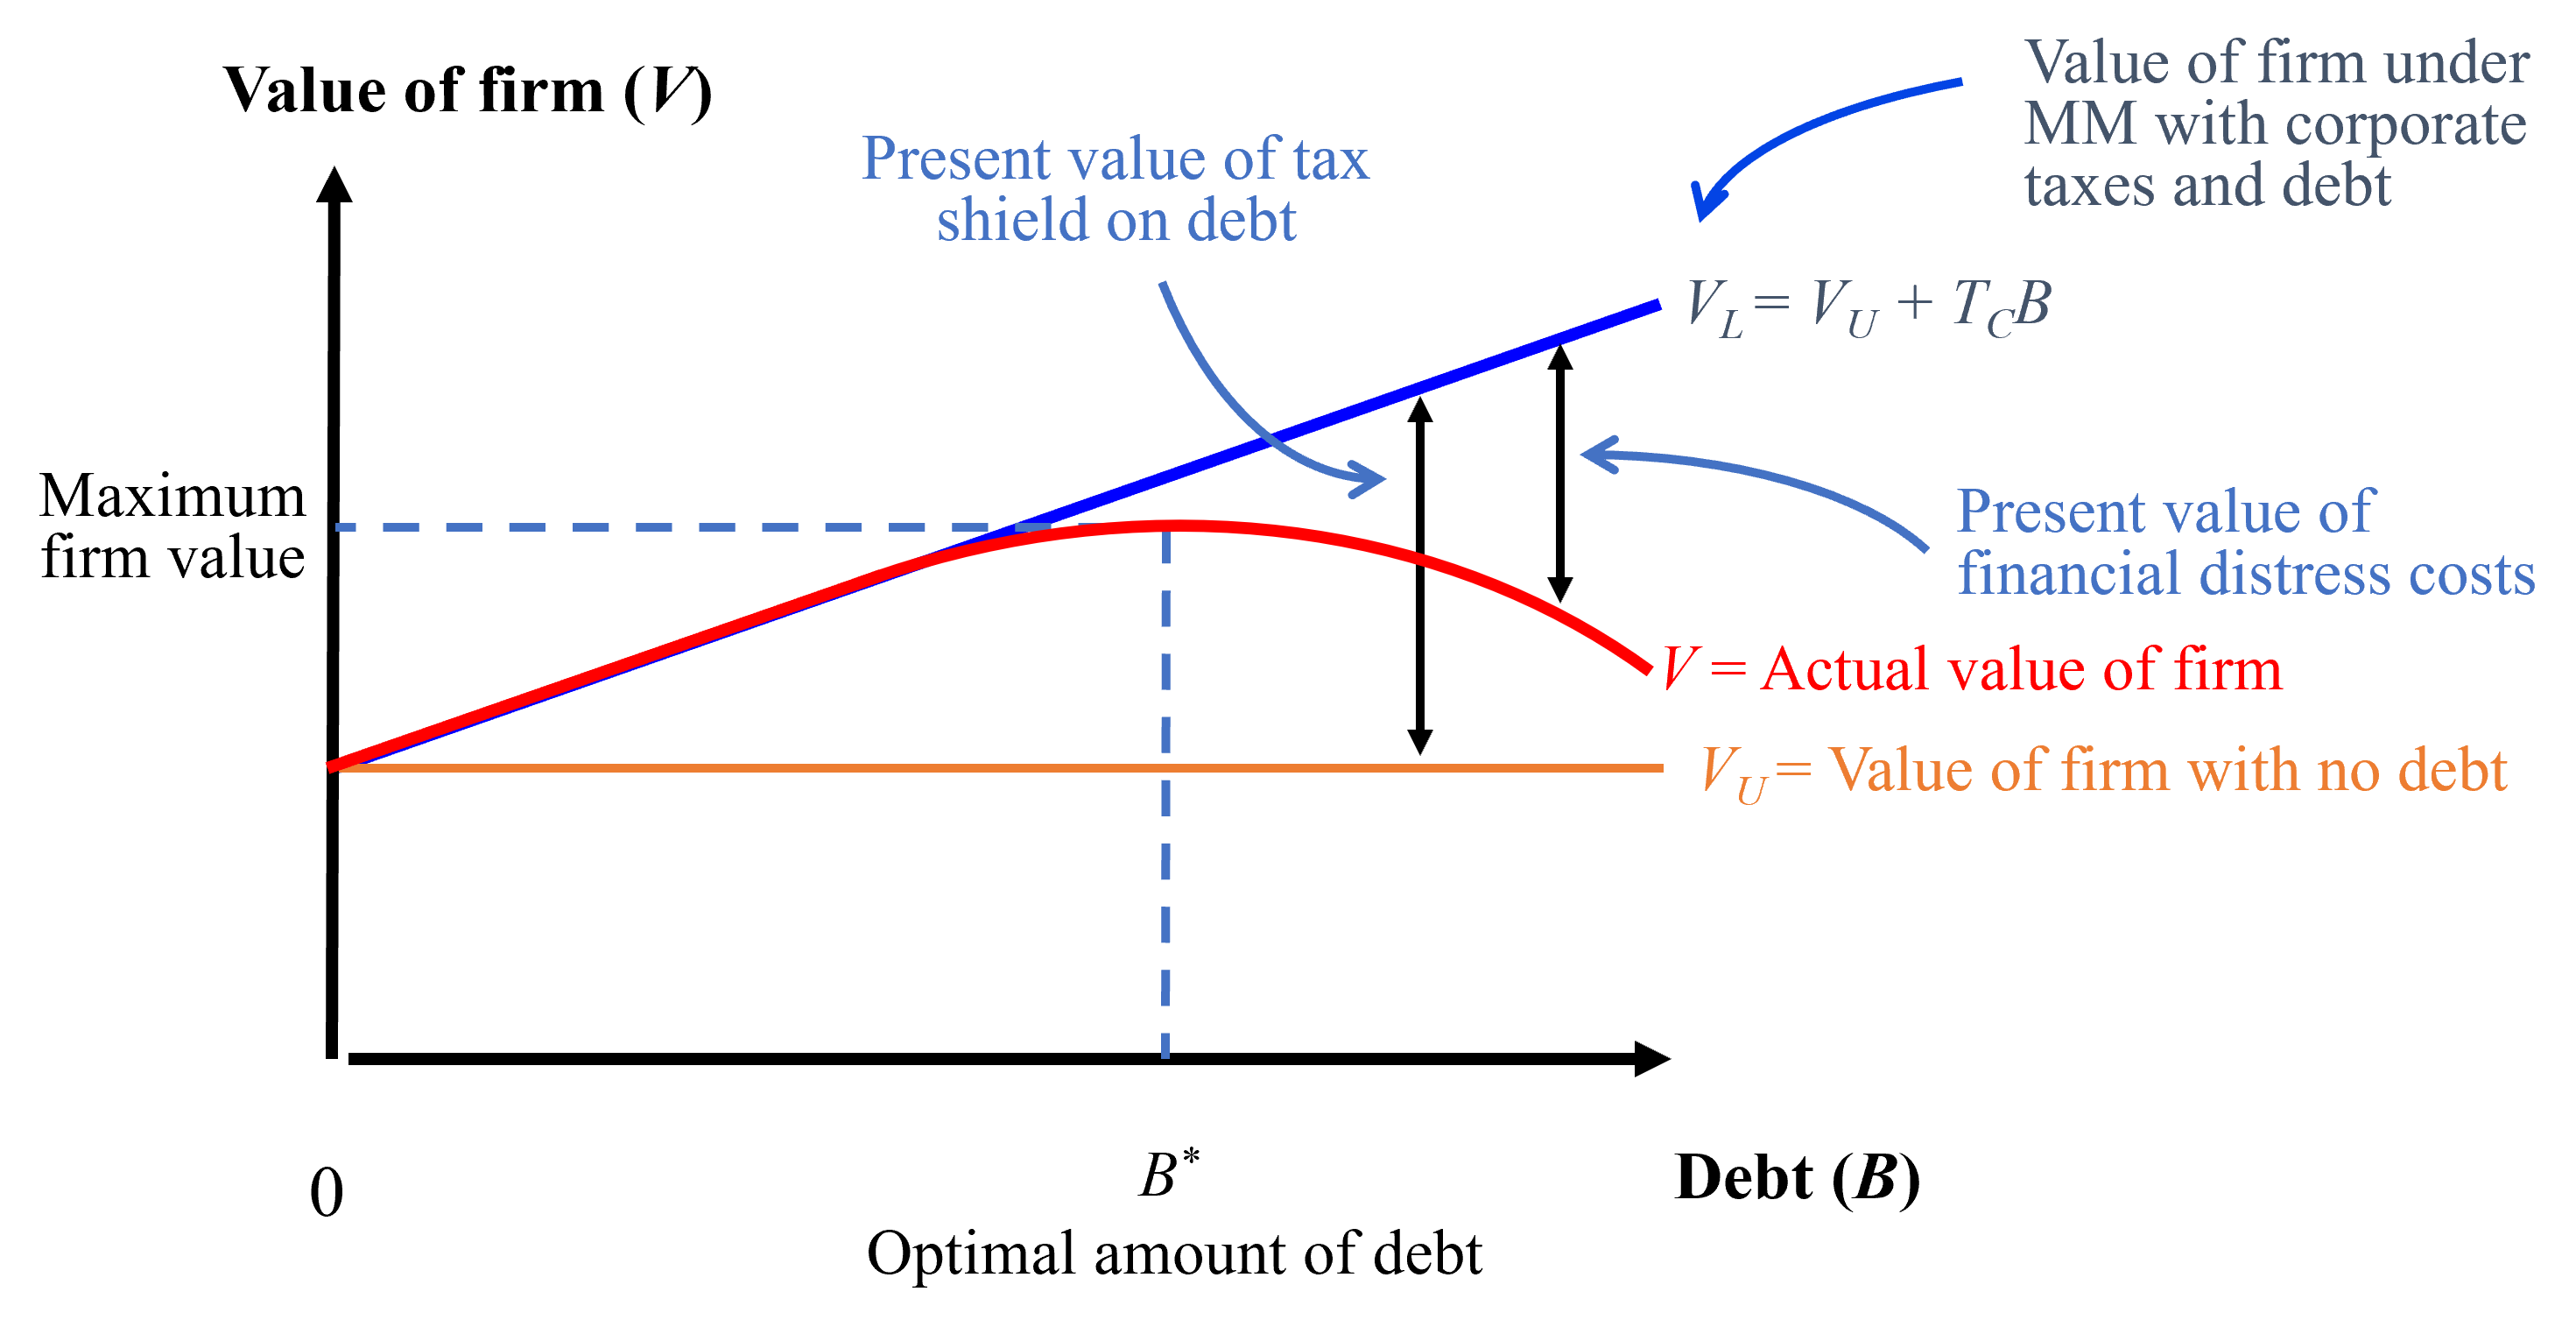
\includegraphics[width=0.7\textwidth]{images/section3/optimaldbratio.png}
		\caption*{\tiny Optimal capital structure occurs before distress costs outweigh tax benefits}
	\end{figure}
	
\end{frame}

\begin{frame}{WACC and the Optimal Capital Structure}
	
	\begin{columns}
		\column{0.52\textwidth}
		\begin{itemize}
			\item The capital structure that \textbf{maximizes firm value} is also the one that \textbf{minimizes WACC}.
			\item Initially, debt lowers WACC due to:
			\begin{itemize}
				\item Lower after-tax cost of debt
			\end{itemize}
			\item Beyond a certain point:
			\begin{itemize}
				\item Higher debt → higher risk → higher \( R_D \) and \( R_E \)
				\item WACC starts to rise
			\end{itemize}
		\end{itemize}
		
		\column{0.48\textwidth}
		\begin{figure}
			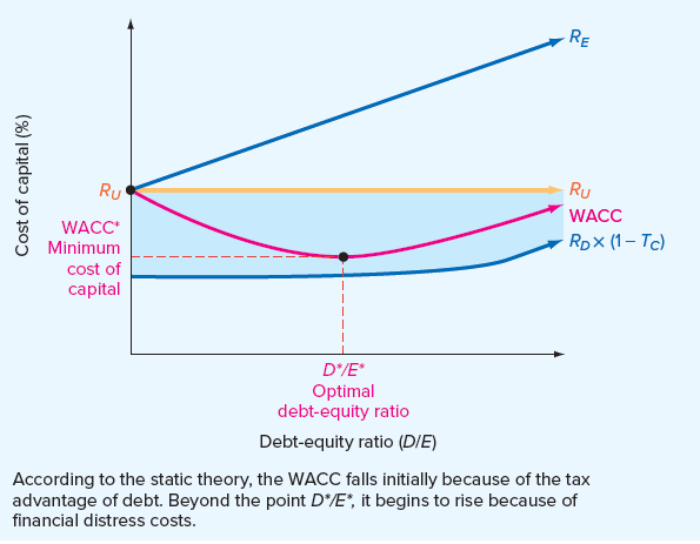
\includegraphics[width=\linewidth]{images/section3/minimalwacc.png}
		\end{figure}
		
	\end{columns}
	
\end{frame}

\begin{frame}{Summary: M\&M Cases and Optimal Capital Structure}
	
	\begin{itemize}
		\item \textbf{Case I: No Taxes, No Bankruptcy Costs}
		\begin{itemize}
			\item Firm value independent of capital structure
			\item \textcolor{gray}{→ No optimal capital structure}
		\end{itemize}
		
		\vspace{2mm}
		\item \textbf{Case II: Corporate Taxes Only}
		\begin{itemize}
			\item Debt creates tax shields → increases firm value
			\item \textcolor{gray}{→ Optimal capital structure = nearly 100\% debt}
		\end{itemize}
		
		\vspace{2mm}
		\item \textbf{Case III: Taxes + Distress Costs}
		\begin{itemize}
			\item Value of debt is offset by expected cost of distress
			\item \textcolor{gray}{→ Optimal capital structure: part debt, part equity}
		\end{itemize}
	\end{itemize}
	
	\vspace{0.2cm}
	\begin{alertblock}{Bottom Line}
		Capital structure matters only when frictions like taxes and bankruptcy costs are present.
	\end{alertblock}
	
\end{frame}

\begin{frame}{M\&M Framework: Comparing Case I, II, and III}
	
	\begin{table}[ht]
		\centering
		\resizebox{\textwidth}{!}{
			\begin{tabular}{lccc}
				\toprule
				\textbf{Dimension} & \textbf{Case I} & \textbf{Case II} & \textbf{Case III} \\
				\midrule
				Taxes & \faTimesCircle None & \faCheckCircle Corporate taxes & \faCheckCircle Corporate taxes \\
				Bankruptcy Costs & \faTimesCircle None & \faTimesCircle None & \faCheckCircle Present \\
				\midrule
				Effect of Debt on Firm Value & None & Increases value via tax shield & Increases value, but with diminishing returns \\
				Optimal Capital Structure & Irrelevant & Almost 100\% debt & Moderate debt level \\
				Cost of Equity \(R_S\) & Increases with leverage & Increases with leverage & Increases faster due to distress risk \\
				WACC & Constant & Decreases with debt & U-shaped: minimized at intermediate debt \\
				\bottomrule
			\end{tabular}
		}
	\end{table}
	
	\vspace{0.2cm}
	\begin{alertblock}{Key Insight}
		Debt is most valuable in Case II. In the real world (Case III), the optimal capital structure is a trade-off between tax benefits and distress costs.
	\end{alertblock}
	
\end{frame}


\begin{frame}{Managerial Implications for Capital Structure}
	
	\textbf{How should managers think about debt?}
	
	\begin{itemize}
		\item \textbf{Tax Position of the Firm}
		\begin{itemize}
			\item Firms with higher and stable taxable income benefit more from debt.
		\end{itemize}
		
		\item \textbf{Financial Distress Risk}
		\begin{itemize}
			\item Firms with volatile EBIT or low asset tangibility should use less debt.
			\item Industry-specific distress costs can vary significantly.
		\end{itemize}
		
		\item \textbf{Practical Guidance:}
		\begin{itemize}
			\item No “one-size-fits-all” solution.
			\item Capital structure must reflect firm fundamentals and risk tolerance.
		\end{itemize}
	\end{itemize}
	
\end{frame}

\subsection{The Extended Pie Model and Broader Stakeholder Claims}
\begin{frame}{The Extended Pie Model: Cash Flows and All Stakeholders}
	
	\textbf{Core Idea:}  
	Capital structure decisions affect not just shareholders and bondholders, but all claimants on the firm’s cash flows.
	
	\vspace{0.3cm}
	\begin{itemize}
		\item \textbf{Taxes:}  
		Increased debt reduces taxes — decreasing the government’s claim on cash flows.
		
		\item \textbf{Bankruptcy Costs:}  
		As leverage increases, the expected value of legal and administrative costs rises.
		
		\item \textbf{All Claims Come from One Source:}
		\[
		\begin{aligned}
			CF &= \text{SUM(stockholders + creditors + gov + courts + others)}
		\end{aligned}
		\]
	\end{itemize}
	
	\vspace{0.3cm}
	\begin{alertblock}{Extended Pie View}
		The firm’s total cash flow supports both \textit{marketed} and \textit{nonmarketed} claims.
	\end{alertblock}
	
\end{frame}

\begin{frame}{The Extended Pie: A Visual Perspective}
	
	\begin{figure}
		\centering
		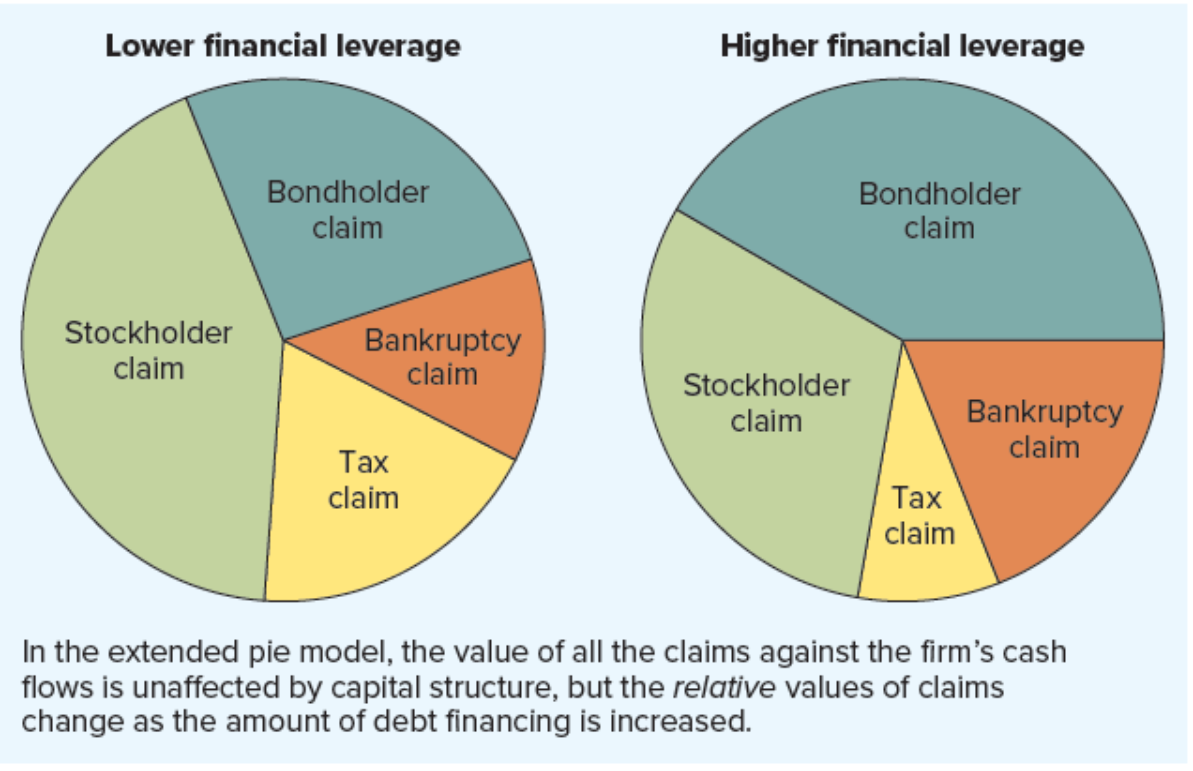
\includegraphics[width=0.9\textwidth]{images/section3/pieII}
	\end{figure}
	
%	\vspace{0.3cm}
%	\textbf{Interpretation:}  
%	When the pie is sliced differently via capital structure changes, the size of some slices (like taxes or distress costs) changes too — affecting marketed claimants.
	
\end{frame}

\begin{frame}{Marketed vs. Nonmarketed Claims}
	
	\textbf{Who has a claim on the firm's cash flows?}
	
	\vspace{0.2cm}
	\begin{itemize}
		\item \textbf{Marketed Claims:}
		\begin{itemize}
			\item Shareholders, bondholders
			\item Traded in financial markets → priced explicitly
		\end{itemize}
		
		\item \textbf{Nonmarketed Claims:}
		\begin{itemize}
			\item Government (taxes), lawyers (bankruptcy fees), communities (externalities)
			\item Cannot be traded but still consume firm resources
		\end{itemize}
	\end{itemize}
	
	\vspace{0.3cm}
	\[
	V_T = V_M + V_N = \text{Total Firm Value}
	\]
	
	\vspace{0.2cm}
	\textbf{Capital structure decisions may shift value between} $V_M$ and $V_N$.
\end{frame}

\begin{frame}{Capital Structure and Broader Stakeholders: A CSR Link}
	
	\textbf{Why Extended Pie Theory Matters in Modern Finance:}
	
	\begin{itemize}
		\item Firms increasingly face scrutiny not just from investors, but also:
		\begin{itemize}
			\item Governments (tax strategies)
			\item Local communities (employment, environmental impacts)
			\item Employees and supply chains
		\end{itemize}
		
		\item \textbf{Capital structure affects these stakeholders:}
		\begin{itemize}
			\item High debt may reduce tax payments, but increase risk to employees or local economies
			\item Aggressive financial policy may reduce long-term reputational capital
		\end{itemize}
	\end{itemize}
	
	\vspace{0.2cm}
	\begin{alertblock}{Strategic Implication}
		The optimal capital structure must increasingly account for \textbf{nonmarketed claims and CSR concerns}.
	\end{alertblock}
	
\end{frame}

\subsection{Beyond Trade-Off: Other Capital Structure Theories}


\subsubsection{Agency Costs of Equity}
\begin{frame}{Agency Costs of Equity: Incentives and Ownership}
	
	\textbf{\textcite{jensen1976theory}} argue that the separation of ownership and control leads to incentive misalignment.
	
	\vspace{0.3cm}
	\begin{itemize}
		\item When managers own a smaller share of the firm (e.g., after issuing new equity), they:
		\begin{itemize}
			\item Have weaker incentives to maximize firm value
			\item May increase consumption of perks or pursue pet projects
			\item May reduce effort or adopt low-value investments
		\end{itemize}
		
		\item Investors anticipate such behavior:
		\begin{itemize}
			\item → New equity may be undervalued in the market
			\item → Managers may avoid issuing equity even when needed
		\end{itemize}
	\end{itemize}
	
	\vspace{0.2cm}
	\begin{alertblock}{Capital Structure Implication}
		Firms with severe equity agency costs may prefer debt to preserve managerial discipline.
	\end{alertblock}
	
\end{frame}


\begin{frame}{Agency Incentives in Action: Ms. Pagell's Dilemma}
	
	\textbf{Owner-manager chooses between debt and equity to raise \$2M.}
	
	\begin{itemize}
		\item More ownership retained under debt → stronger work incentives.
		\item Less ownership under equity → lower incentive to exert effort.
	\end{itemize}
	
	\vspace{0.3cm}
	\begin{table}
		\centering
		\resizebox{0.95\textwidth}{!}{
			\begin{tabular}{@{}lrrrrrrr@{}}
				\toprule
				& & \multicolumn{3}{c}{\textbf{Debt Issue}} & \multicolumn{3}{c}{\textbf{Stock Issue}} \\ \midrule
				\textbf{Work Hours} & \textbf{CF} & \textbf{Interest} & \textbf{Equity CF} & \textbf{To Pagell} & \textbf{Interest} & \textbf{Equity CF} & \textbf{To Pagell} \\
				6-hour/day  & 300K & 240K & 60K & 60K   & 0 & 300K & 100K \\
				10-hour/day & 400K & 240K & 160K & 160K & 0 & 400K & 133K \\
				\bottomrule
			\end{tabular}
		}
	\end{table}
	
\end{frame}

\begin{frame}{Equity Dilution and Incentive Losses}
	
	\begin{itemize}
		\item As equity increases:
		\begin{itemize}
			\item Ownership becomes dispersed
			\item Managers exert less effort
			\item Free cash flow may be wasted
		\end{itemize}
		
		\item \textbf{Equity valuation drops} in anticipation of these behaviors.
		
		\item \textbf{Debt can improve firm value through:}
		\begin{enumerate}
			\item Tax shield benefit
			\item Reducing equity agency costs
			\item But: Increases expected distress costs
		\end{enumerate}
	\end{itemize}
	
\end{frame}

\subsubsection{Free Cash Flow Hypothesis}
\begin{frame}{Free Cash Flow and the Disciplinary Role of Debt}
	
	\begin{block}{Free Cash Flow Hypothesis \parencite{jensen1986agency}}
		Managers overinvest or consume perks when firms have excess free cash flow.
	\end{block}
	
	\vspace{0.3cm}
	\begin{itemize}
		\item \textbf{Higher Dividends}: Reduces cash under managerial control.
		\item \textbf{Higher Debt}:  
		\begin{itemize}
			\item Forces regular payments
			\item Leaves less slack for empire building or perquisite consumption
		\end{itemize}
		\item \textbf{Key Idea:}  
		Debt disciplines management by committing cash flow to external claimants.
	\end{itemize}
	
\end{frame}

\subsubsection{Signaling}
\begin{frame}{Capital Structure as a Signal of Firm Quality}
	
	\textbf{\textcite{ross1977signaling}} developed a theory in which \textbf{capital structure conveys private information} about firm quality to investors.
	
	\vspace{0.3cm}
	\begin{itemize}
		\item \textbf{Assumption:}  
		Managers know the true value of the firm, investors do not.
		
		\item \textbf{Mechanism:}  
		High-quality firms take on more debt to \textbf{signal confidence}.  
		\begin{itemize}
			\item Debt increases financial risk, which low-quality firms are unwilling to bear.
		\end{itemize}
		
		\item \textbf{Equilibrium:}  
		Investors interpret higher leverage as a signal of higher firm value — but only if signaling is \textbf{costly to mimic}.
		
		\item Over-leveraging beyond the optimal level imposes long-term costs (bankruptcy, loss of credibility).
	\end{itemize}
	
\end{frame}

\begin{frame}{Signaling: Why Only High-Quality Firms Take on More Debt?}
	
	\textbf{To be effective, signals must be costly for low-quality firms to mimic.}
	
	\vspace{0.3cm}
	\begin{table}[ht]
		\centering
		\resizebox{0.9\textwidth}{!}{
			\begin{tabular}{lcc}
				\toprule
				\textbf{Firm Type} & \textbf{High Quality (HQ)} & \textbf{Low Quality (LQ)} \\
				\midrule
				Private Info      & High future cash flow        & High bankruptcy risk \\
				Incentive to Signal via Debt? & \faCheckCircle Yes – want to distinguish & \faTimesCircle No – risk too costly \\
				Investor Belief   & "More debt → high quality"   & "Less debt → low quality" \\
				Equilibrium Action & Choose higher debt           & Choose lower debt \\
				\bottomrule
			\end{tabular}
		}
	\end{table}
	
	\vspace{0.2cm}
	\textbf{Conclusion:}  
	Debt acts as a \textbf{credible signal} of firm quality only if the signaling cost (financial distress) deters mimicking by LQ firms.
\end{frame}

\subsubsection{The Pecking Order Theory}
\begin{frame}{Financing Hierarchy: The Pecking Order Theory}
	
	\textbf{Pecking Order Theory} provides an alternative to static capital structure theories like trade-off theory.
	
	\begin{itemize}
		\item Proposed by \textcite{myers1984corporate}, it emphasizes the role of \textbf{information asymmetry} in financing decisions.
		\item Firms follow a hierarchical preference when financing investments:
		\begin{enumerate}
			\item Internal Funds (Retained Earnings)
			\item Debt Financing
			\item Equity Issuance (last resort)
		\end{enumerate}
		\item Firms avoid equity because it signals possible overvaluation to outside investors.
	\end{itemize}
	
	\vspace{0.2cm}
	\begin{alertblock}{Key Assumption}
		Managers know more than investors — issuing equity may signal “bad news.”
	\end{alertblock}
	
\end{frame}

\begin{frame}{Why the Pecking Order Emerges: Three Drivers}
	
	\textbf{Three key reasons why internal funds are preferred:}
	
	\vspace{0.3cm}
	\begin{itemize}
		\item \textbf{(1) Cost Minimization:}
		\begin{itemize}
			\item Internal funds avoid issuance costs.
			\item Debt incurs interest but offers tax deductibility.
		\end{itemize}
		
		\item \textbf{(2) Signaling Effects:}
		\begin{itemize}
			\item Equity issuance may be interpreted as “firm is overvalued.”
			\item Debt signals confidence without overly negative inference.
		\end{itemize}
		
		\item \textbf{(3) Control Preservation:}
		\begin{itemize}
			\item Equity dilutes ownership and control rights.
		\end{itemize}
	\end{itemize}
	
\end{frame}

\begin{frame}{The Pecking Order in Practice}
	
	\begin{columns}
		\column{0.5\textwidth}
		\textbf{The Financing Sequence:}
		\begin{itemize}
			\item First: Retained Earnings
			\item Then: Debt (until capacity reached)
			\item Last: Equity
		\end{itemize}
		
		\vspace{0.3cm}
		\textbf{Implication:}
		\begin{itemize}
			\item More profitable firms use less debt
			\item Less profitable firms issue more debt or equity
		\end{itemize}
		
		\column{0.5\textwidth}
		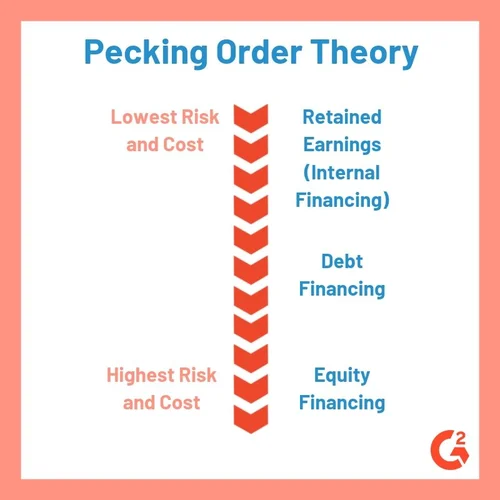
\includegraphics[width=\linewidth]{images/section3/peckingorder.png}
	\end{columns}
	
\end{frame}

\begin{frame}{Behavioral Implications of the Pecking Order}
	
	\textbf{Key Characteristics:}
	
	\begin{itemize}
		\item Firms do not target a specific debt-equity ratio.
		\item Capital structure evolves over time based on financing needs.
		\item More profitable firms tend to:
		\begin{itemize}
			\item Accumulate internal funds
			\item Avoid issuing equity
			\item Maintain low leverage
		\end{itemize}
		\item Firms value \textbf{financial slack}:
		\begin{itemize}
			\item Buffer to finance future investments
			\item Avoid negative signaling from external financing
		\end{itemize}
	\end{itemize}
	
\end{frame}

\begin{frame}{Pecking Order vs. Trade-Off Theory}
	
	\begin{table}[ht]
		\centering
		\resizebox{0.95\textwidth}{!}{
			\begin{tabular}{lcc}
				\toprule
				\textbf{Dimension} & \textbf{Trade-Off Theory} & \textbf{Pecking Order Theory} \\
				\midrule
				Key Driver & Tax benefits vs. distress cost & Information asymmetry \\
				Target D/E Ratio & Yes, optimal level exists & No target ratio \\
				Firm Behavior & Optimize WACC & Minimize info cost \\
				Leverage & Profitable firms use more debt & Profitable firms use less debt \\
				Focus & Long-run capital structure & Short-run financing tactics \\
				\bottomrule
			\end{tabular}
		}
	\end{table}
	
\end{frame}

\subsubsection{Dynamic Rebalancing Theory}
\begin{frame}{Dynamic Rebalancing Theory}
	
	\textbf{Do firms continuously adjust their capital structure toward an optimal level?}
	
	\begin{itemize}
		\item In theory (e.g., trade-off model), firms rebalance when leverage drifts from target.
		\item In reality, adjustments are \textbf{infrequent and partial}.
		\item Reasons for delayed rebalancing:
		\begin{itemize}
			\item Adjustment costs (transaction fees, signaling concerns)
			\item Managerial inattention or inertia
			\item Financial flexibility preferences
		\end{itemize}
		\item Empirical evidence:  
		\textcite{leary2005revolving} find most firms adjust slowly — often only when issuing external capital.
	\end{itemize}
	
	\vspace{0.3cm}
	\textbf{Implication:}  
	Observed leverage is often a result of past shocks and only gradually moves back toward target.
	
\end{frame}

\subsubsection{Market Timing Theory}
\begin{frame}{Market Timing Theory}
	
	\textbf{What if capital structure is just a by-product of timing past financing windows?}
	
	\begin{itemize}
		\item Firms issue equity when stock prices are high (perceived overvaluation).
		\item Firms issue debt when interest rates are low or stock price is undervalued.
		\item No target D/E ratio is needed — structure reflects historical timing.
	\end{itemize}
	
	\vspace{0.3cm}
	\textbf{Key Study:}  
	\textcite{baker2002market} show firms that issued equity during high valuations have persistently lower leverage over time.
	
	\vspace{0.3cm}
	\begin{alertblock}{Conclusion}
		Capital structure reflects \textbf{cumulative outcomes of past market conditions}, not just firm fundamentals.
	\end{alertblock}
	
\end{frame}

\subsubsection*{Alternative Capital Structure Theory}
\begin{frame}{Summary: Alternative Capital Structure Theories}
	
	\begin{table}[ht]
		\centering
		\resizebox{\textwidth}{!}{
			\begin{tabular}{lllll}
				\toprule
				\textbf{Theory} & \textbf{Key Driver} & \textbf{Mechanism} & \textbf{Prediction on Leverage} & \textbf{Notes} \\
				\midrule
				Agency Costs of Equity & Ownership–control sep & Equity dilution weakens managerial incentives & Higher debt improves effort alignment & \textcite{jensen1976theory} \\
				Free Cash Flow & Empire building risk & Debt limits managerial discretion & More debt when cash flow is high & \textcite{jensen1986agency} \\
				Signaling Theory & Private info asymmetry & High-quality firms use more debt & High debt = high quality signal & \textcite{ross1977signaling} \\
				Pecking Order Theory & Info asymmetry + cost & Internal > debt > equity & Profitable firms use less debt & \textcite{myers1984corporate} \\
				Dynamic Rebalancing & Adjustment costs & Partial, slow return to target & D/E drifts over time & \textcite{leary2005revolving} \\
				Market Timing Theory & Valuation windows & Issue equity when overvalued & Structure reflects timing history & \textcite{baker2002market} \\
				\bottomrule
			\end{tabular}
		}
	\end{table}
	
	\vspace{0.2cm}
	\textbf{Conclusion:} These theories complement the traditional trade-off framework by incorporating behavior, information, and dynamics.
	
\end{frame}


\subsection{How Firms Establish Capital Structure in Practice}
\begin{frame}{Capital Structures Vary Widely Across Countries}
	
	\begin{figure}
		\centering
		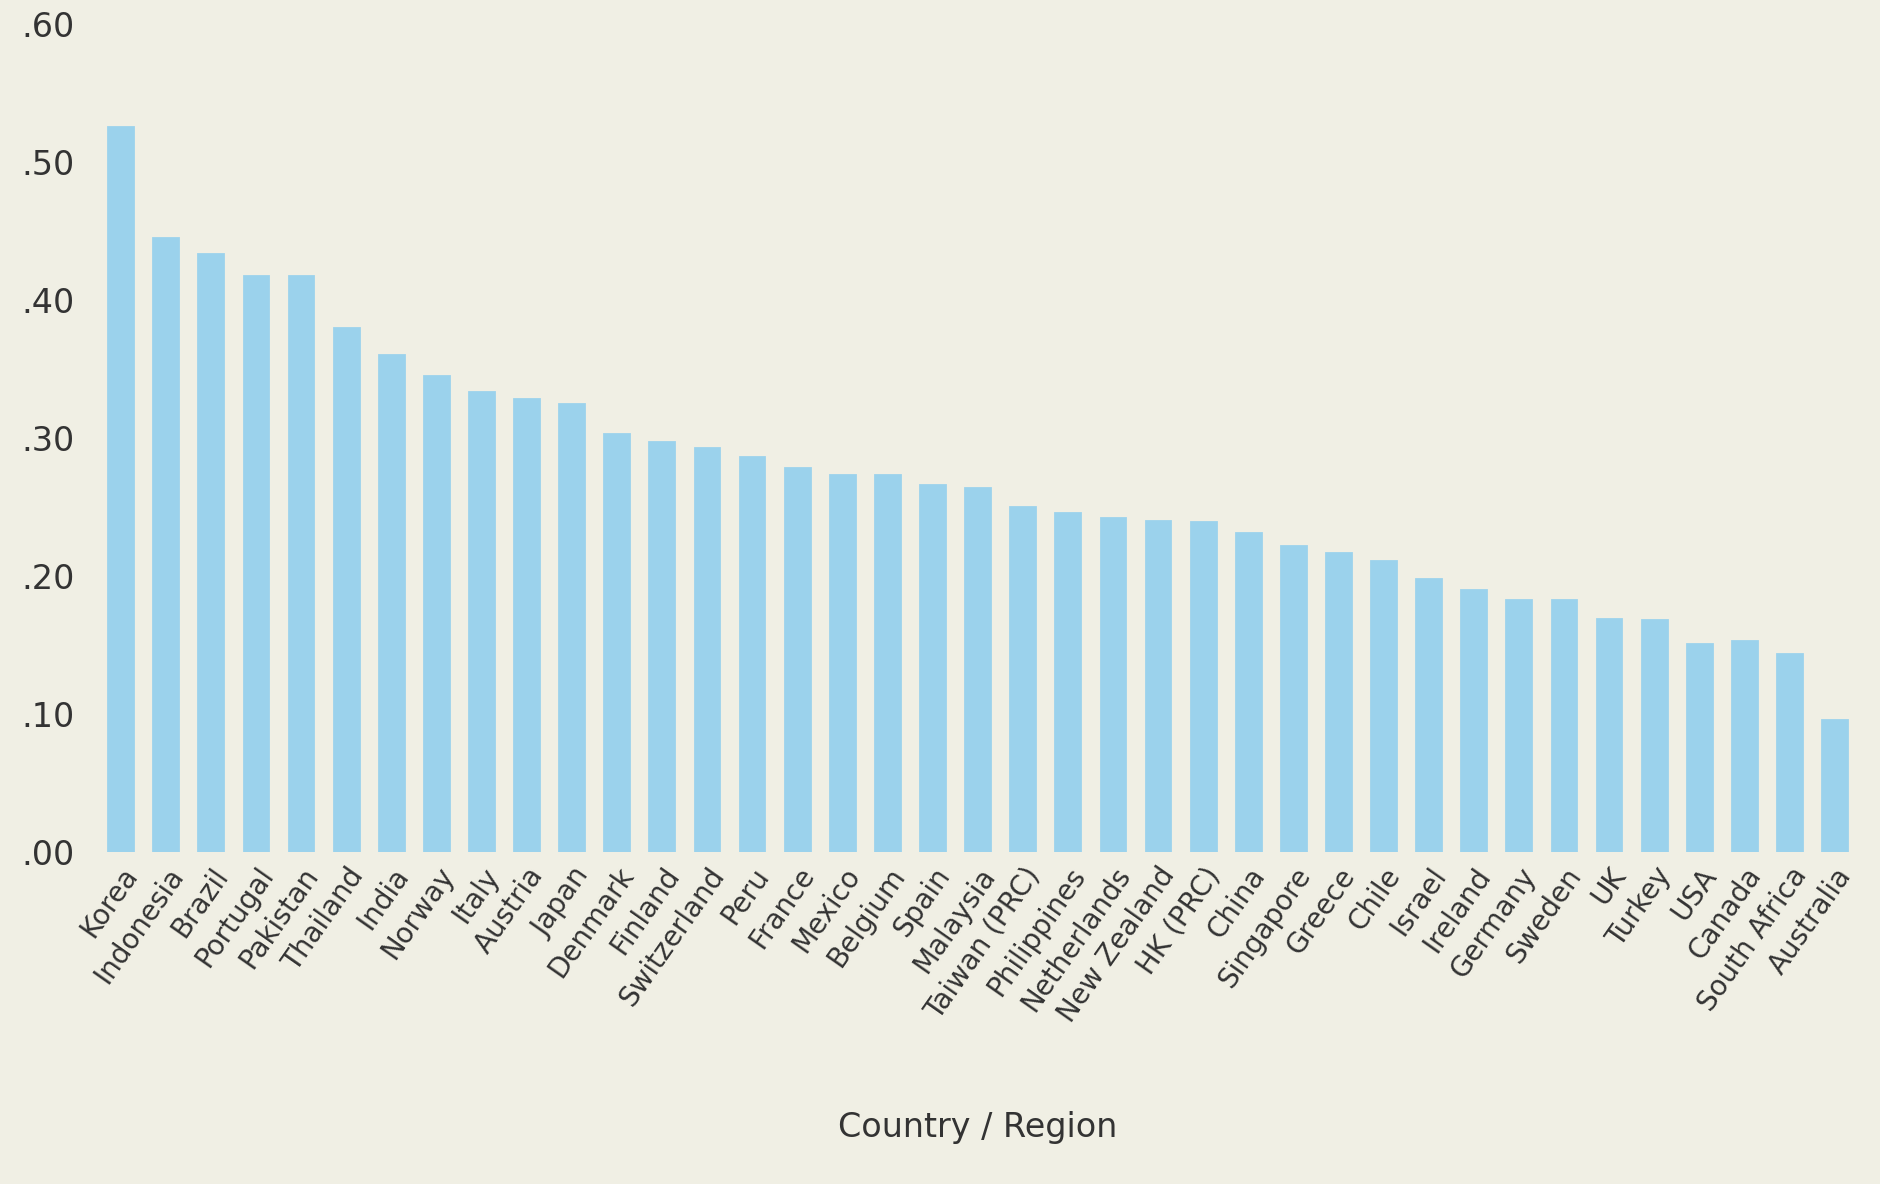
\includegraphics[width=0.85\textwidth]{images/section3/internationaldbratio.png}
	\end{figure}
	
	\tiny{Source: \textcite{fan2012international}. Shows median debt-to-assets ratios across countries.}
	
	\textbf{Observation:} Even in the absence of global theory consensus, capital structure is influenced by tax laws, legal protections, and institutional quality.
\end{frame}
\begin{frame}{Most Firms Maintain a Target Capital Structure}
	
	\begin{figure}
		\centering
		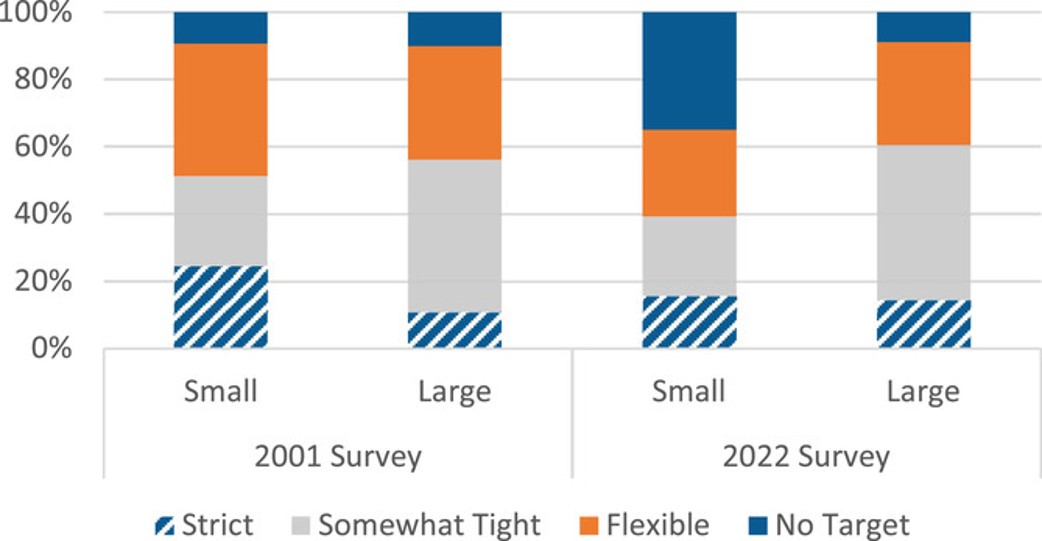
\includegraphics[width=0.85\textwidth]{images/section3/targetdebt.jpg}
	\end{figure}
	
	\tiny{Source: \textcite{graham2022presidential}. Survey evidence: Firms differ in how strictly they follow D/E targets.}
	
	\vspace{2mm}
	\textbf{Key Insight:} Most firms (especially large ones) maintain a target debt ratio — but many adopt flexible or somewhat loose adherence.
\end{frame}
\begin{frame}{Firm-Level Capital Structures Are Not Static}
	
	\begin{columns}
		% Left: Image
		\begin{column}{0.4\textwidth}
			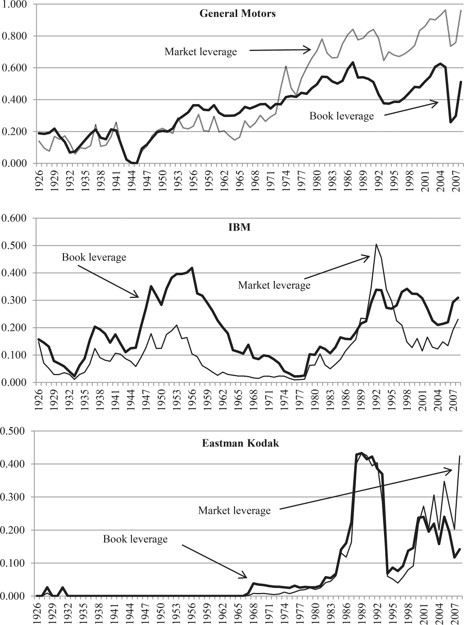
\includegraphics[width=\linewidth]{images/section3/csvariation.jpg}\\
			\tiny{Source: \textcite{deangelo2015stability}}
		\end{column}
		
		% Right: Text
		\begin{column}{0.6\textwidth}
			\textbf{Key Insight:} \\
			Capital structure targets are often long-term — in the short run, observed leverage can deviate significantly.
			
			\vspace{0.4cm}
			\textbf{Why does leverage drift?}
			\begin{itemize}
				\item Changes in market equity value (denominator)
				\item Internal equity financing via retained earnings
				\item No immediate need to rebalance
			\end{itemize}
			
			\vspace{0.3cm}
			\textbf{Implication:} Leverage ratios are dynamic, even for firms with long-run targets.
		\end{column}
	\end{columns}
	
\end{frame}

\begin{frame}{Capital Structures Differ by Industry}
	
	\begin{figure}
		\centering
		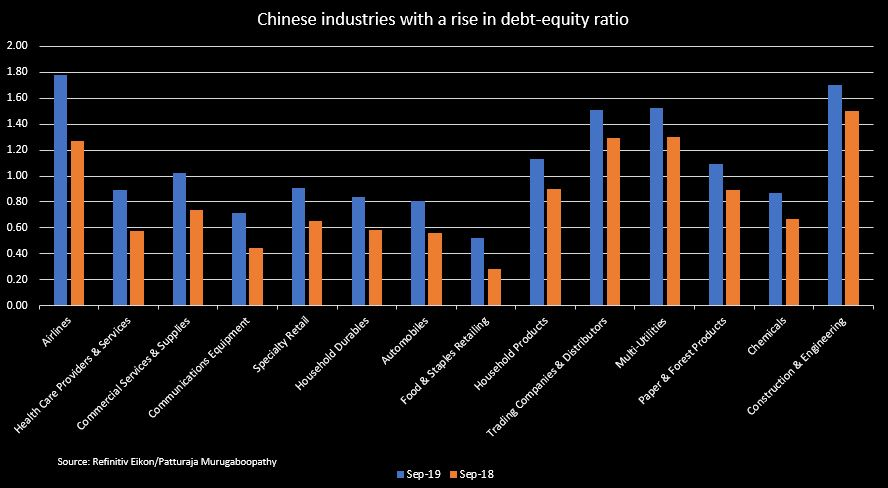
\includegraphics[width=0.9\textwidth]{images/section3/cnderatio.jpg}
	\end{figure}
	
	\tiny{Source: Refinitiv / Reuters. Leverage varies based on operating risk and asset type.}
	
	\vspace{2mm}
	\textbf{Example:} Airlines and utilities exhibit high leverage; tech and services often rely more on equity.
\end{frame}
\begin{frame}{What Determines a Firm’s Target D/E Ratio?}
	
	\begin{itemize}
		\item \textbf{Taxes:}
		\begin{itemize}
			\item Interest tax shield encourages more debt for profitable firms.
		\end{itemize}
		
		\item \textbf{Asset Tangibility:}
		\begin{itemize}
			\item Tangible assets provide collateral → lower distress costs → higher debt capacity.
			\item Firms with intangible assets (e.g., R\&D) favor equity.
		\end{itemize}
		
		\item \textbf{Earnings Volatility:}
		\begin{itemize}
			\item More volatile EBIT increases risk of distress → encourages equity financing.
		\end{itemize}
	\end{itemize}
	
	\vspace{2mm}
	\textbf{Additional factors:} growth opportunities, managerial preferences, macro conditions.
	
\end{frame}
\begin{frame}{Empirical Realities of Capital Structure: Key Takeaways}
	
	\begin{itemize}
		\item \textbf{Capital structure is context-specific} — shaped by:
		\begin{itemize}
			\item Institutional environment (e.g., legal systems, taxation)
			\item Industry characteristics (e.g., asset tangibility, volatility)
			\item Firm attributes (e.g., size, profitability, lifecycle stage)
		\end{itemize}
		
		\item \textbf{Target leverage ratios exist}, but are often flexible bands rather than precise points.
		
		\item \textbf{Observed capital structure fluctuates} due to:
		\begin{itemize}
			\item Market valuation changes
			\item Internal financing and retained earnings
			\item Timing or adjustment costs
		\end{itemize}
		
		\item \textbf{Theory provides a framework}, but real-world capital structure reflects both rational design and practical constraints.
	\end{itemize}
	
\end{frame}

\subsection*{Summary}
\begin{frame}{Summary: Capital Structure and Its Limits}
	\footnotesize
	\textbf{1. Why Not 100\% Debt?} \\
	\begin{itemize}
		\item Debt provides tax shields, but...
		\item \textcolor{red}{Bankruptcy costs} (direct + indirect) reduce firm value
		\item \textcolor{red}{Agency conflicts} (e.g., risk-shifting, underinvestment)
	\end{itemize}
	
	\textbf{2. Main Theories Beyond MM} \\
	\begin{itemize}
		\item \textbf{Trade-Off Theory:} Balance tax benefits and distress costs
		\item \textbf{Agency Theory:} Debt disciplines managers; equity dilutes incentives
		\item \textbf{Signaling Theory:} High leverage = signal of firm quality
		\item \textbf{Pecking Order:} Internal $>$ Debt $>$ Equity (due to asymmetric info)
		\item \textbf{Market Timing \& Rebalancing:} Structure reflects past opportunities
	\end{itemize}
	
	\textbf{3. Real-World Implications} \\
	\begin{itemize}
		\item Most firms maintain flexible target ranges for D/E
		\item Leverage varies across \textbf{countries, industries, firm types}
		\item Capital structure reflects both \textit{rational design} and \textit{practical constraints}
	\end{itemize}
	
\end{frame}

\begin{frame}{Discussion: Which Theory Best Fits China?}
	
	\textbf{Question:}  
	Which capital structure theory best explains the financing behavior of firms in China?
	
	\begin{itemize}
		\item \textbf{Trade-Off Theory}
		\begin{itemize}
			\item Does the tax shield dominate firm decisions?
			\item How important are bankruptcy costs in SOEs vs. private firms?
		\end{itemize}
		
		\item \textbf{Pecking Order Theory}
		\begin{itemize}
			\item Do firms avoid equity due to asymmetric information?
			\item What is the role of internal funds and retained earnings?
		\end{itemize}
		
		\item \textbf{Agency / Free Cash Flow}
		\begin{itemize}
			\item How does concentrated ownership affect managerial behavior?
			\item Are high cash firms more likely to over-invest?
		\end{itemize}
		
		\item \textbf{Market Timing}
		\begin{itemize}
			\item Do Chinese firms issue equity in “hot” markets?
			\item Are IPO waves driven by valuation windows?
		\end{itemize}
	\end{itemize}
	
	\textbf{Follow-up:}  
	Can one theory explain all firms? Or do different types (SOEs, tech, exporters) follow different models?
	
\end{frame}


% \section{Valuation and Capital Budgeting for the Levered Firm}
% \begin{frame}{Valuation and Capital Budgeting for the Levered Firm}
	
	\textbf{Core Question:}  
	How do we value investment projects when the firm uses both debt and equity financing?
	
	\vspace{0.3cm}
	\begin{itemize}
		\item \textbf{Why It Matters:}  
		Capital budgeting and valuation must reflect financing choices -- taxes, interest, risk all change with leverage.
		
		\item \textbf{Challenges with Leverage:}
		\begin{itemize}
			\item Project risk is no longer the same as firm risk
			\item Discount rates must account for debt usage
			\item Tax shields and financial distress impact value
		\end{itemize}
		
		\item \textbf{This Section Covers Three Valuation Methods:}
		\begin{enumerate}
			\item \textbf{Adjusted Present Value (APV)} -- separates project value from financing side effects
			\item \textbf{Flow to Equity (FTE)} -- values equity cash flows directly
			\item \textbf{WACC} -- most commonly used, integrates risk and capital costs
		\end{enumerate}
		
		\item \textbf{Application:}  
		We’ll also discuss how to estimate discount rates and betas when direct comparables are unavailable.
	\end{itemize}
	
\end{frame}

\subsection{Adjusted Present Value}
\begin{frame}{Adjusted Present Value (APV)}
	
	\begin{block}{Formula}
		\[
		\text{APV} = \text{NPV (unlevered)} + \text{NPV of Financing Effects (NPVF)}
		\]
	\end{block}
	
	\begin{itemize}
		\item \textbf{Core Idea:}  
		Start with an unlevered project valuation, then add/subtract effects from financing choices.
		
		\item \textbf{Why use APV?}
		\begin{itemize}
			\item Financing effects (e.g., tax shields) can be valued separately.
			\item Especially useful when leverage is changing or financing is non-standard.
		\end{itemize}
		
		\item \textbf{Common NPVF Components:}
		\begin{itemize}
			\item Tax shield from debt
			\item Issuance costs of equity or debt
			\item Subsidized debt (e.g., government lending)
			\item Expected distress costs
		\end{itemize}
	\end{itemize}
	
\end{frame}
\begin{frame}{APV Example: Step 1 – Unlevered NPV}
	
	\textbf{Project: Nio Inc.}
	
	\begin{itemize}
		\item Perpetual project with:
		\begin{itemize}
			\item Revenue = ¥5,000,000 per year
			\item Costs = ¥3,830,380 per year
			\item Initial Investment = ¥4,750,000
			\item Tax rate: \( T_C = 21\% \), Cost of capital: \( R_0 = 20\% \)
		\end{itemize}
		
		\item \textbf{Unlevered After-Tax Cash Flow}:
		\[
		\text{UCF} = (5,000,000 - 3,830,380) \times (1 - 0.21) = \text{\textyen}924,000
		\]
		
		\item \textbf{NPV (Unlevered)}:
		\[
		NPV = -4,750,000 + \frac{924,000}{0.20} = -\text{\textyen}130,000
		\]
		
		\item $\rightarrow$ Without financing help, project should be \textcolor{red}{rejected}.
	\end{itemize}
	
\end{frame}
\begin{frame}{APV Example: Step 2 – Add Subsidized Financing Effect}
	
	\begin{itemize}
		\item Assume Hefei government provides a permanent debt subsidy of ¥1,219,000
		\item Tax shield from debt:
		\[
		\text{NPVF} = T_C \times \text{Debt} = 0.21 \times 1,219,000 = \text{\textyen}255,990
		\]
		
		\item \textbf{Adjusted Present Value:}
		\[
		\text{APV} = -\text{\textyen}130,000 + \text{\textyen}255,990 = \text{\textyen}125,990
		\]
		
		\item $\rightarrow$ \textbf{Accept} the project: government support turned a negative NPV project into a positive one.
	\end{itemize}
	
\end{frame}

\subsection{Flow to Equity Approach}
\begin{frame}{Flow to Equity (FTE) Valuation Method}
	
	\textbf{Core Idea:}  
	Value a project by forecasting cash flows to equity holders and discounting at the cost of levered equity \( R_S \).
	
	\vspace{0.3cm}
	\begin{block}{Formula}
		\[
		\text{Value}_{\text{Equity}} = \frac{\text{Levered Cash Flows (LCF)}}{R_S}
		\]
	\end{block}
	
	\vspace{0.2cm}
	\textbf{Three Steps:}
	\begin{enumerate}
		\item Estimate LCF: Project cash flows after interest and taxes
		\item Estimate \( R_S \): Cost of equity using levered beta or MM II
		\item Discount LCFs using \( R_S \)
	\end{enumerate}
	
	\vspace{0.2cm}
	\textbf{When to Use:}
	\begin{itemize}
		\item Useful when capital structure is fixed and financing effects are embedded in cash flows.
	\end{itemize}
	
\end{frame}

\begin{frame}{Step 1: Estimate Levered Cash Flows (LCF)}
	
	\textbf{Nio Project Assumptions (Perpetuity):}
	\begin{itemize}
		\item Revenues: ¥5,000,000, Costs: ¥3,830,380
		\item Debt: ¥1,219,000 at 10\% $\rightarrow$ Interest = ¥121,900
		\item Tax rate: \( T_C = 21\% \)
	\end{itemize}
	
	\textbf{Step-by-step LCF:}
	\begin{table}[]
		\centering
		\begin{tabular}{lr}
			\toprule
			Revenue             & ¥5,000,000 \\
			Operating Cost      & ¥3,830,380 \\
			EBIT                & ¥1,169,620 \\
			Interest Payment    & ¥121,900 \\
			\midrule
			EBT                 & ¥1,047,720 \\
			Taxes (21\%)        & ¥220,021 \\
			\midrule
			\textbf{LCF}        & ¥827,699 \\
			\bottomrule
		\end{tabular}
	\end{table}
	
\small
	Alternatively:  
	\[
	\text{LCF} = \text{UCF} - (1 - T_C) \cdot R_B \cdot B = \text{\textyen}827,699
	\]
	
\end{frame}

\begin{frame}{Step 2: Compute Levered Cost of Equity \( R_S \)}
	
	\textbf{MM Proposition II (with taxes):}
	\[
	R_S = R_0 + \frac{B}{S}(1 - T_C)(R_0 - R_B)
	\]
	
	\vspace{0.2cm}
	\textbf{In our example:}
	\begin{itemize}
		\item \( R_0 = 20\%, R_B = 10\%, T_C = 21\% \)
		\item Total project value = ¥4,876,000 $\rightarrow$ Equity = ¥3,657,000
		\item \( B/S = 1,219,000 / 3,657,000 \approx \frac{1}{3} \)
	\end{itemize}
	
	\vspace{0.2cm}
	\[
	R_S = 0.20 + \frac{1}{3} \cdot (1 - 0.21) \cdot (0.20 - 0.10) = 0.2263
	\]
	
\end{frame}

\begin{frame}{Step 3: Valuation Using FTE}
	
	\begin{itemize}
		\item \textbf{Value of equity (project):}
		\[
		\text{PV}_{\text{Equity}} = \frac{LCF}{R_S} = \frac{\text{\textyen}827,699}{0.2263} = \text{\textyen}3,656,990
		\]
		
		\item \textbf{Equity outlay:}
		\[
		\text{Equity Invested} = \text{\textyen} 4,750,000 - \text{\textyen}1,219,000 = \text{\textyen}3,531,000
		\]
		
		\item \textbf{NPV to equityholders:}
		\[
		\text{\textyen}3,656,990 - \text{\textyen}3,531,000 = \text{\textyen}125,990
		\]
		
		\item $\rightarrow$ Project should be \textbf{accepted} from the equityholders’ point of view.
	\end{itemize}
	
\end{frame}
\subsection{WACC}
\begin{frame}{WACC Method: Weighted Average Cost of Capital}
	\textbf{Definition:}  
	WACC reflects the firm's blended cost of capital, accounting for both debt and equity, after taxes.
	\begin{block}{Formula}
		\[
		WACC = \frac{S}{S + B} \cdot R_S + \frac{B}{S + B} \cdot (1 - T_C) \cdot R_B
		\]
	\end{block}
	
	\textbf{Key Concept:}
	\begin{itemize}
		\item Use \textbf{unlevered cash flows} (UCFs) from the project.
		\item Discount them at the firm’s WACC to obtain total firm/project value.
	\end{itemize}
	\textbf{In our Nio example:}
	\begin{itemize}
		\item \( R_S = 22.63\% \), \( R_B = 10\% \), \( T_C = 21\% \)
		\item Capital structure: \( S:B = 3:1 \Rightarrow w_E = 0.75, w_D = 0.25 \)
		\item \[
		WACC = 0.75 \cdot 0.2263 + 0.25 \cdot 0.79 \cdot 0.10 = 18.95\%
		\]
	\end{itemize}
\end{frame}

\begin{frame}{WACC Valuation Example}
	
	\textbf{Recall:} Unlevered after-tax cash flow (UCF) = ¥924,000 per year (perpetuity)
	
	\vspace{0.2cm}
	\textbf{Project Value (using WACC):}
	\[
	V = \frac{\text{\textyen}924,000}{0.1895} = \text{\textyen}4,876,000
	\]
	
	\textbf{Initial investment = ¥4,750,000}
	
	\vspace{0.3cm}
	\textbf{Net Present Value (NPV):}
	\[
	NPV = \text{\textyen}4,876,000 - \text{\textyen}4,750,000 = \text{\textyen}125,990
	\]
	
	\vspace{0.2cm}
	\textbf{Conclusion:}  
	Same result as APV and FTE -- all methods should yield consistent NPV if inputs are used correctly.
	
\end{frame}
\begin{frame}{Comparing APV, FTE, and WACC}
	
	\textbf{Goal:} All three methods aim to value a project with leverage.
	
	\vspace{0.3cm}
	\textbf{How They Differ:}
	\begin{itemize}
		\item \textbf{WACC:} Incorporates tax shield into the discount rate
		\item \textbf{FTE:} Values equity cash flows directly
		\item \textbf{APV:} Separates project value from financing effects
	\end{itemize}
	
	\vspace{0.3cm}
	\textbf{Which to Use?}
	\begin{itemize}
		\item Use \textbf{WACC} or \textbf{FTE} if firm maintains a constant target D/V ratio over time
		\item Use \textbf{APV} when the financing side is nonstandard (e.g., fixed debt schedule, subsidies, restructuring)
	\end{itemize}
	
	\vspace{0.3cm}
	\textbf{Practice Tip:}  
	In industry, \textbf{WACC is the most widely used} due to simplicity and convention.
	
\end{frame}
\begin{frame}{Summary: APV vs. FTE vs. WACC}
	
	\begin{table}
		\resizebox{\textwidth}{!}{\begin{tabular}{llll}
				\toprule
				\textbf{Feature} & \textbf{APV} & \textbf{WACC} & \textbf{FTE} \\
				\midrule
				Initial Investment & Total project cost & Total project cost & Equity only \\
				
				Cash Flows Used & Unlevered cash flows (UCF) & UCF & Levered cash flows (LCF) \\
				
				Discount Rate & \( R_0 \) (unlevered) & \( WACC \) (after-tax) & \( R_S \) (levered equity) \\
				
				Tax Shield Treatment & Separate cash flow item (added) & Built into discount rate & Built into LCFs \\
				
				Best When & Debt schedule is known & D/V ratio is constant & Focus is on equity returns \\
				
				Popularity in Practice & Common in academia & Most used in practice & Less common \\
				\bottomrule
		\end{tabular}}
	
	\end{table}
	
	
	\vspace{0.3cm}
	\textbf{Bottom Line:}  
	All three methods should give the same result if used consistently.
	
\end{frame}

\subsection{Applications of Levered Valuation Techniques}
\subsubsection{World-Wide Enterprises}
\begin{frame}{Estimating a Discount Rate: WWE Widget Example}
	
	\begin{block}{Context}
		World-Wide Enterprises (WWE) is evaluating entry into the widget business. It plans to use a 25\% debt-to-value ratio for all widget projects.
	\end{block}
	
	\vspace{0.2cm}
	\textbf{Industry Benchmark: American Widgets (AW)}
	\begin{itemize}
		\item Capital structure: 40\% debt / 60\% equity
		\item Equity beta: \( \beta_E = 1.5 \)
		\item Borrowing rate: 12\%
	\end{itemize}
	
	\vspace{0.2cm}
	\textbf{Assumptions:}
	\begin{itemize}
		\item WWE's widget borrowing rate: 10\%
		\item Risk-free rate: 8\%
		\item Market risk premium: 8.5\%
		\item Corporate tax rate: 21\%
	\end{itemize}
	
	\vspace{0.2cm}
	\textbf{Goal:}  
	Estimate WWE’s appropriate discount rate for its widget venture.
	
\end{frame}
\begin{frame}{Step 1: Estimate Unlevered Return \( R_0 \) from Industry Proxy}
	
	\textbf{Step 1a: Compute AW’s cost of equity using CAPM}
	\[
	R_S^{AW} = R_F + \beta_E \cdot (R_M - R_F) = 0.08 + 1.5 \cdot 0.085 = \textbf{20.75\%}
	\]
	
	\vspace{0.3cm}
	\textbf{Step 1b: Solve for unlevered cost of capital \( R_0 \)}  
	Using MM Proposition II (with taxes):
	\[
	R_S = R_0 + \frac{B}{S}(1 - T_C)(R_0 - R_B)
	\]
	
	\[
	0.2075 = R_0 + \frac{0.4}{0.6} \cdot 0.79 \cdot (R_0 - 0.12)
	\]
	
	Solving gives:  
	\[
	\boxed{R_0 = 17.73\%}
	\]
	
	\textbf{Interpretation:}  
	This is WWE's project cost of capital if financed entirely with equity.
	
\end{frame}
\begin{frame}{Step 2: Estimate WWE's \( R_S \) and WACC}
	
	\textbf{Step 2a: Cost of equity for WWE’s capital structure (25\% debt)}
	\[
	R_S^{WWE} = R_0 + \frac{B}{S}(1 - T_C)(R_0 - R_B)
	\]
	
	\[
	= 0.1773 + \frac{0.25}{0.75} \cdot 0.79 \cdot (0.1773 - 0.10) = \boxed{19.77\%}
	\]
	
	\vspace{0.3cm}
	\textbf{Step 2b: Compute WACC for WWE's widget projects}
	\[
	WACC = w_D \cdot R_B (1 - T_C) + w_E \cdot R_S
	\]
	
	\[
	= 0.25 \cdot 0.10 \cdot 0.79 + 0.75 \cdot 0.1977 = \boxed{16.80\%}
	\]
	
	\vspace{0.2cm}
	\textbf{Conclusion:}  
	Use \textbf{16.80\%} to discount unlevered project cash flows in capital budgeting.
	
\end{frame}

\subsubsection{Bicksler Enterprises}
\begin{frame}{Bicksler Enterprises: Project Setup (All-Equity Baseline)}
	
	\begin{block}{Project Details}
		\begin{itemize}
			\item Initial investment: \$10,000,000
			\item Project life: 5 years
			\item Straight-line depreciation: \$2,000,000/year
			\item Cash revenues $–$ expenses: \$3,500,000/year
			\item Corporate tax rate: 21\%
			\item Risk-free rate: 10\%, Unlevered cost of capital: 20\%
		\end{itemize}
	\end{block}
	
	\textbf{Cash Flow Estimates (in \$ thousands):}
	\vspace{-3mm}
	\begin{table}[]
		\centering
		\resizebox{\textwidth}{!}{
			\begin{tabular}{lrrrrrr}
				\toprule
				& Year 0 & Year 1 & Year 2 & Year 3 & Year 4 & Year 5 \\
				\midrule
				Initial Outlay & -10,000 &       &       &       &       &       \\
				Depreciation Tax Shield &        & 420   & 420   & 420   & 420   & 420 \\
				Net After-Tax Revenue &          & 2,765 & 2,765 & 2,765 & 2,765 & 2,765 \\
				\bottomrule
			\end{tabular}
		}
	\end{table}
	
\end{frame}

\begin{frame}{Step 1: All-Equity Project Valuation}
	
	\textbf{Present Value Calculations (in \$):}
	\begin{itemize}
		\item Depreciation tax shield (risk-free):
		\[
		PV_{\text{Dep}} = \frac{420{,}000}{0.10} \cdot \left[1 - \frac{1}{1.10^5}\right] = \text{\$1,592,130}
		\]
		\item After-tax operating CF:
		\[
		PV_{\text{Revenue}} = \frac{2,765{,}000}{0.20} \cdot \left[1 - \frac{1}{1.20^5}\right] = \text{\$8,269,043}
		\]
	\end{itemize}
	
	\vspace{2mm}
	\textbf{All-Equity NPV:}
	\[
	NPV = -10,000,000 + 1,592,130 + 8,269,043 = \textcolor{red}{-\$138,827}
	\]
	
	\textbf{Conclusion:} Project would be rejected under all-equity financing.
	
\end{frame}

\begin{frame}{Step 2: Debt Flotation Costs and Tax Shield}
	
	\textbf{Debt Raised:} \$7,500,000 net after flotation  
	\textbf{Gross proceeds:}
	\[
	\text{Gross} = \frac{7,500,000}{1 - 0.01} = 7,575,758
	\]
	
	\textbf{Flotation cost = \$75,758; amortized over 5 years (straight line)}
	
	\vspace{1mm}
	\textbf{Annual Tax Shield:}
	\[
	\text{Tax Shield} = 21\% \cdot 15,152 = 3,182
	\]
	
	\textbf{PV of Tax Shield on Flotation Costs:}
	\[
	PV = \frac{3,182}{0.10} \cdot \left[1 - \frac{1}{1.10^5}\right] = 12,062
	\]
	
	\textbf{Net flotation cost:}
	\[
	-75,758 + 12,062 = \textcolor{red}{-\$63,696}
	\]
	
\end{frame}

\begin{frame}{Step 3: Tax Shield from Interest Payments}
	
	\textbf{Loan amount:} \$7,575,758 at 10\% interest  
	\textbf{Annual Interest = \$757,576; After-tax = \$598,485}
	
	\vspace{2mm}
	\textbf{PV of Interest Tax Shield:}
	\[
	PV = 7,575,758 - \frac{598,485}{0.10} \cdot \left[1 - \frac{1}{1.10^5}\right] - \frac{7,575,758}{1.10^5}
	\]
	\[
	= \textcolor{blue}{\$603,080}
	\]
	
	\textbf{Interpretation:} This is the value of subsidized debt net of interest burden.
	
\end{frame}

\begin{frame}{Step 4: Adjusted Present Value (with Debt)}
	
	\textbf{Summary:}
	\begin{itemize}
		\item All-Equity NPV = \textcolor{red}{-\$138,827}
		\item Net flotation cost = \textcolor{red}{-\$63,696}
		\item Debt value (NPV of tax subsidy) = \textcolor{blue}{\$603,080}
	\end{itemize}
	
	\vspace{2mm}
	\[
	APV = -138,827 - 63,696 + 603,080 = \boxed{\text{\$400,557}}
	\]
	
	\textbf{Conclusion:}  
	$\rightarrow$ Project should be \textbf{accepted} if debt financing is available.
	
\end{frame}

\begin{frame}{Step 5: Subsidized Financing -- State Loan at 8\%}
	
	\textbf{Loan = \$7,500,000 at 8\% interest, no flotation costs}
	
	\textbf{Annual after-tax interest:}
	\[
	\$600,000 \cdot (1 - 0.21) = \$474,000
	\]
	
	\textbf{NPV of subsidized loan:}
	\[
	NPV = 7,500,000 - \frac{474,000}{0.10} \cdot \left[1 - \frac{1}{1.10^5}\right] - \frac{7,500,000}{1.10^5}
	= \boxed{\$1,046,257}
	\]
	
\end{frame}

\begin{frame}{Final APV with Subsidized Loan}
	
	\textbf{All-Equity NPV:} \textcolor{red}{-\$138,827}  
	\textbf{+ Subsidized Loan NPV:} \textcolor{blue}{\$1,046,257}
	
	\[
	\text{APV} = -138,827 + 1,046,257 = \boxed{\$907,430}
	\]
	
	\textbf{Conclusion:}  
	$\rightarrow$ Subsidized financing significantly enhances project value.  
	$\rightarrow$ Governments can make socially beneficial projects financially viable.
	
\end{frame}
\subsection{Beta and Leverage}
\begin{frame}{Beta and Leverage with Corporate Taxes}
	
	\begin{block}{Beta of Levered Equity (with risk-free debt)}
		If debt is risk-free ($\beta_B = 0$), the levered equity beta is:
		\begin{equation}
			\beta_S = \left[1 + \frac{B}{S}(1 - T_C)\right] \beta_0
			\label{eq:betalever}
		\end{equation}
	\end{block}
	
	\vspace{0.3cm}
	\textbf{Intuition:} Financial leverage increases the equity beta due to the magnification of operating risk.
	
	\vspace{0.2cm}
	\textbf{Assumption:} This holds when the firm's debt is risk-free and perpetual.
	
\end{frame}

\begin{frame}{Decomposing Firm Beta under Leverage}
	
	\begin{itemize}
		\item Total firm beta is a weighted average of security betas:
		\begin{equation}
			\beta_L = \frac{B}{V_L} \beta_B + \frac{S}{V_L} \beta_S
			\label{eq:betal}
		\end{equation}
		
		\item It can also be expressed in terms of asset value and tax shield:
		\begin{equation}
			\beta_L = \frac{V_0}{V_L} \beta_0 + \frac{T_C B}{V_L} \beta_B
			\label{eq:betatc}
		\end{equation}
	\end{itemize}
	
	\pause
	\textbf{Where:}
	\begin{itemize}
		\item $\beta_0$: unlevered (asset) beta
		\item $\beta_B$: beta of debt
		\item $V_0$: unlevered firm value; $V_L$: levered firm value
	\end{itemize}
	
\end{frame}

\begin{frame}{Derivation: When $\beta_B = 0$}
	
	\begin{itemize}
		\item Equating \eqref{eq:betal} and \eqref{eq:betatc}, and assuming $\beta_B = 0$:
		\begin{align*}
			\frac{S}{V_L} \beta_S &= \frac{V_0}{V_L} \beta_0\\
			\Rightarrow \beta_S &= \frac{V_0}{S} \beta_0 = \left[1 + \frac{B}{S}(1 - T_C)\right] \beta_0
		\end{align*}
		
		\item \textbf{Result:} $\beta_S > \beta_0$, i.e., leverage increases equity risk.
		
		\pause
		\item When debt is risky ($\beta_B \neq 0$):
		\begin{equation*}
			\beta_S = \beta_0 + \frac{B}{S}(1 - T_C)(\beta_0 - \beta_B)
		\end{equation*}
	\end{itemize}
	
\end{frame}

\begin{frame}{Example: Unlevering Equity Beta}
	
	\begin{block}{Example Setup}
		C. F. Lee, Inc. has \$100M in debt and \$200M in equity. Debt is risk-free. Equity beta is 2. Corporate tax rate is 21\%.
		
		\vspace{0.2cm}
		What is the appropriate discount rate for a new project if it were financed with equity only?
	\end{block}
	
	\vspace{0.2cm}
	\textbf{Given:}
	\begin{itemize}
		\item $\beta_S = 2$, $B = 100$, $S = 200$, $T_C = 0.21$
		\item $R_F = 10\%$, $E(R_M) - R_F = 8.5\%$
	\end{itemize}
	
\end{frame}

\begin{frame}{Solution: Unlevered Discount Rate}
	
	\begin{itemize}
		\item Step 1: Compute unlevered beta
		\begin{align*}
			\beta_0 &= \frac{S}{S + (1 - T_C) B} \cdot \beta_S \\
			&= \frac{200}{200 + 0.79 \times 100} \cdot 2 = 1.43
		\end{align*}
		
		\pause
		\item Step 2: Compute unlevered cost of equity
		\begin{align*}
			R_0 &= R_F + \beta_0 \cdot [E(R_M) - R_F] \\
			&= 0.10 + 1.43 \times 0.085 = 22.19\%
		\end{align*}
	\end{itemize}
	\pause
	\textbf{Conclusion:} Use 22.19\% to discount unlevered project cash flows.
	
\end{frame}

\subsection*{Summary}
\begin{frame}{Summary: Levered Valuation Techniques}
	\begin{itemize}
		\item \textbf{Goal}: Value investment projects in the presence of leverage.
		\item \textbf{Key Challenges}:
		\begin{itemize}
			\item Financing affects risk, discount rates, and tax exposure.
			\item Need to account for interest tax shields and distress costs.
		\end{itemize}
		\item \textbf{Methods Covered}:
		\begin{itemize}
			\item \textbf{Adjusted Present Value (APV)}: Unlevered NPV + PV of financing effects.
			\item \textbf{Flow to Equity (FTE)}: Discount levered cash flows to equity at $R_S$.
			\item \textbf{WACC}: Discount unlevered cash flows at weighted average cost of capital.
		\end{itemize}
		\item \textbf{Application Topics}:
		\begin{itemize}
			\item Estimating discount rates using comparables
			\item Incorporating flotation costs, subsidies, and beta adjustment
		\end{itemize}
	\end{itemize}
\end{frame}

\begin{frame}{Key Formulas for Levered Firm Valuation}
	\small
	\begin{itemize}
		\item \textbf{APV:} $ \displaystyle APV = \text{NPV}_{\text{unlevered}} + \text{NPV}_{\text{financing effects}} $
		
		\item \textbf{FTE:} $ \displaystyle \text{Equity Value} = \frac{\text{Levered Cash Flows (LCF)}}{R_S} $
		
		\item \textbf{WACC:} $ \displaystyle WACC = \frac{S}{S + B} R_S + \frac{B}{S + B}(1 - T_C) R_B $
		
		\item \textbf{MM Proposition II (with taxes):} 
		$ \displaystyle R_S = R_0 + \frac{B}{S}(1 - T_C)(R_0 - R_B) $
		
		\item \textbf{Levered Beta (with riskless debt):} 
		$ \displaystyle \beta_S = \left[1 + \frac{B}{S}(1 - T_C)\right] \beta_0 $
		
		\item \textbf{Firm Value (WACC or FTE):} 
		$ \displaystyle V = \sum \frac{\text{UCF or LCF}}{\text{Appropriate Rate}} $
	\end{itemize}
\end{frame}


% \section{Dividends and Other Payouts}
% \begin{frame}{Types of Payouts to Shareholders}
\footnotesize
\begin{itemize}
    \item \textbf{Cash Dividends} -- The most common form:
    \begin{itemize}
        \item \textit{Regular cash dividend}: Typically paid quarterly in the U.S.
        \item \textit{Extra dividend}: Paid occasionally when the firm has surplus cash.
        \item \textit{Liquidating dividend}: A one-time payout as the firm winds down.
    \end{itemize}

    \item \textbf{Stock Dividends} -- Paid in the form of additional shares:
    \begin{itemize}
        \item No cash leaves the firm.
        \item Dilutes the ownership percentage but not value.
    \end{itemize}

    \item \textbf{Dividends in Kind} -- Non-cash distribution (rare):
    \begin{itemize}
        \item Example: Wrigley's Gum once sent chewing gum to shareholders.
    \end{itemize}

    \item \textbf{Stock Buybacks} -- An alternative to dividends:
    \begin{itemize}
        \item Reduces the number of shares outstanding.
        \item Can signal undervaluation or distribute temporary cash flows flexibly.
    \end{itemize}
\end{itemize}
\end{frame}

\subsection{Cash Dividend}
\subsubsection{Timeline}
\begin{frame}{Timeline of a Cash Dividend Payment}
\begin{figure}
    \centering
    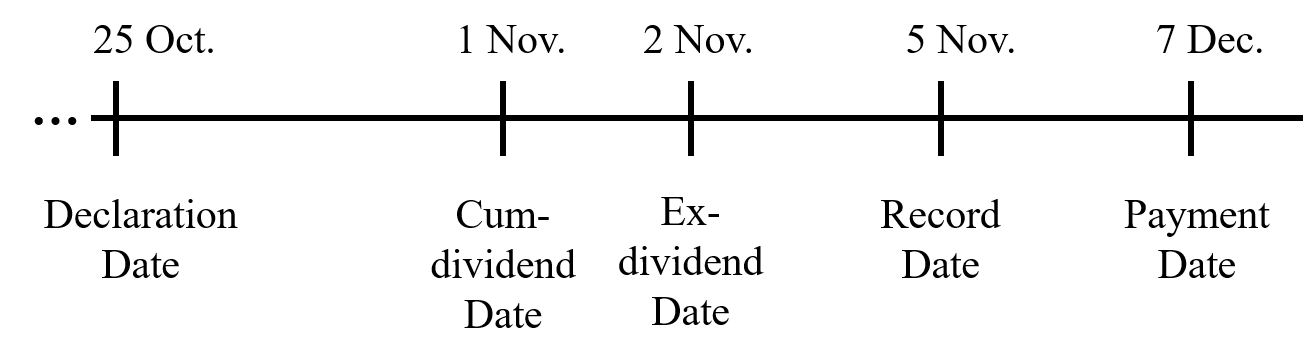
\includegraphics[width=0.9\textwidth]{images/section5/dividendprocess}
\end{figure}
\vspace{-5mm}
\footnotesize
\begin{itemize}
    \item \textbf{Declaration Date}: The board announces the dividend (a legal liability is created).
    \item \textbf{Record Date}: Shareholders on record at this date are entitled to receive the dividend.
    \item \textbf{Ex-Dividend Date}: Typically two business days before the record date. Buyers on or after this date will \textit{not} receive the dividend.
    \item \textbf{Cum-Dividend Date}: The last day when a buyer of the stock still receives the dividend.
    \item \textbf{Payment Date}: The date when dividend checks are mailed or direct deposits made.
\end{itemize}
\end{frame}

\begin{frame}{Apple Inc. (AAPL) Dividend History: 2022-2024}
\footnotesize
\begin{table}[h]
\centering
\resizebox{\textwidth}{!}{
\begin{tabular}{cccccc}
\toprule
\textbf{Ex-Date} & \textbf{Type} & \textbf{Amount} & \textbf{Declaration Date} & \textbf{Record Date} & \textbf{Payment Date} \\
\midrule
05/10/2024 & Cash & \$0.25 & 05/02/2024 & 05/13/2024 & 05/16/2024 \\
02/09/2024 & Cash & \$0.24 & 02/01/2024 & 02/12/2024 & 02/15/2024 \\
11/10/2023 & Cash & \$0.24 & 11/02/2023 & 11/13/2023 & 11/16/2023 \\
08/11/2023 & Cash & \$0.24 & 08/03/2023 & 08/14/2023 & 08/17/2023 \\
05/12/2023 & Cash & \$0.24 & 05/04/2023 & 05/15/2023 & 05/18/2023 \\
02/10/2023 & Cash & \$0.23 & 02/02/2023 & 02/13/2023 & 02/16/2023 \\
11/04/2022 & Cash & \$0.23 & 10/27/2022 & 11/07/2022 & 11/10/2022 \\
08/05/2022 & Cash & \$0.23 & 07/28/2022 & 08/08/2022 & 08/11/2022 \\
05/06/2022 & Cash & \$0.23 & 04/28/2022 & 05/09/2022 & 05/12/2022 \\
02/04/2022 & Cash & \$0.22 & 01/27/2022 & 02/07/2022 & 02/10/2022 \\
\bottomrule
\end{tabular}
}
\end{table}
\vspace{-2mm}
{\tiny Source: NASDAQ}
\end{frame}
\subsubsection{Price Behavior}
\begin{frame}{Price Behavior Around the Ex-Dividend Date}

\small
\textbf{In theory:}  
\vspace{1mm}
\begin{itemize}
    \item In a frictionless market, a stock's price should drop by exactly the amount of the dividend on the \textbf{ex-dividend date}.
\end{itemize}

\vspace{-2mm}
\begin{figure}
    \centering
    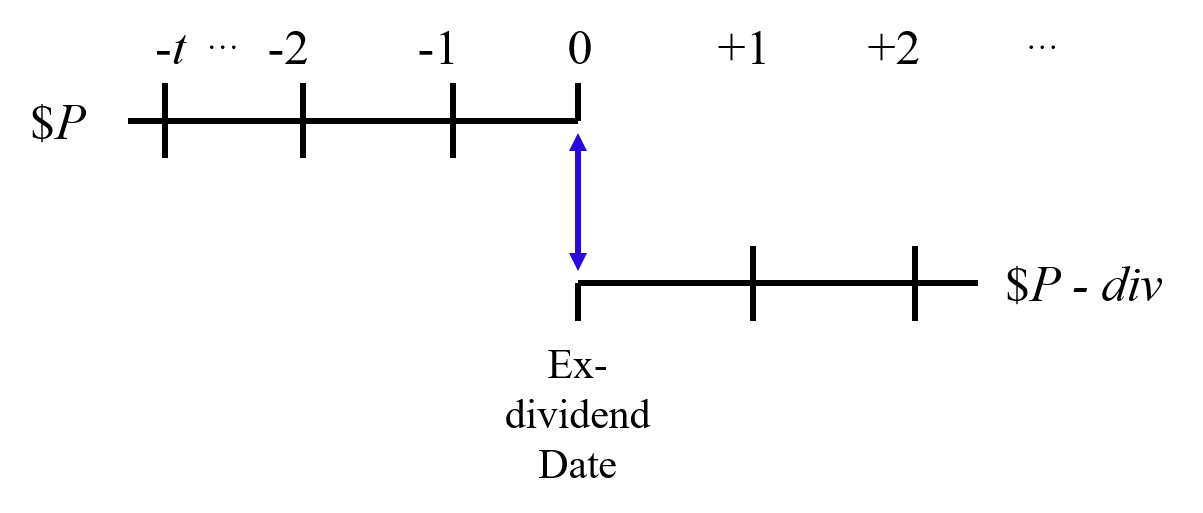
\includegraphics[width=0.75\textwidth]{images/section5/pricebehavior}
\end{figure}
\vspace{-7mm}
\textbf{In practice:}
\begin{itemize}
    \item The price drop is typically \textit{less than the dividend}.
    \item The adjustment usually occurs within minutes of the market opening.
    \item This deviation is primarily due to \textbf{tax preferences} and market microstructure.
\end{itemize}
\end{frame}

\subsubsection{The Irrelevance of Dividend Policy}
\begin{frame}{The Irrelevance of Dividend Policy}

\begin{itemize}
    \item In a perfect capital market, \textbf{dividend policy is irrelevant} to firm value.
    \vspace{2mm}
    \item Investors can create their preferred cash flow stream through \textbf{homemade dividends}:
    \begin{itemize}
        \item Need cash? Sell shares.
        \item Don't want cash? Reinvest dividends.
    \end{itemize}
    \vspace{2mm}
    \item As long as the firm's \textbf{investment policy and total cash flow} remain unchanged, payout decisions do not affect value.
\end{itemize}

\end{frame}

\begin{frame}{Benchmark Case: Bristol Corporation}

\begin{itemize}
    \item Consider a firm with no growth and no investment opportunities.
    \item Bristol Corp. has \$10,000 in cash today and expects \$10,000 more next year, after which it will liquidate.
\end{itemize}

\vspace{3mm}
\begin{center}
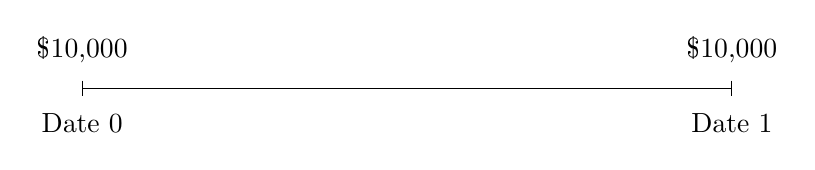
\begin{tikzpicture}[x=1.5cm, y=1cm]
    \draw[-] (0,0) -- (5.5,0);
    \foreach \x in {0,5.5} {
        \draw (\x,0.1) -- (\x,-0.1);
    }
    \node[below] at (0,-0.2) {Date 0};
    \node[below] at (5.5,-0.2) {Date 1};
    \node[above] at (0,0.2) {\$10,000};
    \node[above] at (5.5,0.2) {\$10,000};
\end{tikzpicture}
\end{center}

\begin{itemize}
    \item Discount rate: 10\%
\end{itemize}

\end{frame}

\begin{frame}{Current Policy: Dividend Equals Current Cash Flow}

\begin{itemize}
    \item The firm pays out \$10,000 immediately, and \$10,000 next year.
    \item Present value of the firm:
    \[
        V_0 = \$10,000 + \frac{\$10,000}{1.1} = \$19,090.91
    \]
    \item With 1,000 shares outstanding:
    \[
        P_0 = \$10 + \frac{\$10}{1.1} = \$19.09
    \]
    \item After the dividend, the share price falls to:
    \[
        P_{\text{ex-div}} = \$19.09 - 10 = \$9.09
    \]
\end{itemize}

\end{frame}

\begin{frame}{Alternative Policy: Dividends Greater Than Cash Flow}

\begin{itemize}
    \item Suppose the firm pays a dividend of \$11 per share today.
    \item To finance the extra \$1,000, it issues new equity at \$19.09/share.
    \item New investors expect:
    \[
        \$1,000 \times 1.1 = \$1,100 \text{ return at Date 1}
    \]
    \item Remaining \$8,900 goes to old shareholders:
    \[
        P_0 = \$11 + \frac{\$8.90}{1.1} = \$19.09
    \]
\end{itemize}

\end{frame}

\begin{frame}{The Dividend Indifference Proposition}

\begin{itemize}
    \item Dividend policy does not affect share value if:
    \begin{itemize}
        \item The firm pays out all cash eventually
        \item Capital markets are perfect (no taxes, no transaction costs)
    \end{itemize}
    
    \vspace{2mm}
    \item Investors are indifferent between:
    \begin{itemize}
        \item \textbf{Dividends vs. Capital Gains}: Delayed payouts $\approx$ capital gains
        \item \textbf{Dividends vs. Retained Earnings}: Retained earnings must eventually be distributed
    \end{itemize}
    
    \vspace{2mm}
    \item Homemade dividends replicate any desired cash flow stream
\end{itemize}

\end{frame}

\subsubsection{Homemade Dividends}
\begin{frame}{Homemade Dividends: Investor Preferences}

\begin{itemize}
    \item Investors can adjust their own cash flows to suit their preferences -- regardless of the firm's dividend policy.
    \vspace{3mm}
    
    \item \textbf{Case 1: Investor X prefers smooth dividends of \$10 at Date 0 and Date 1.}
    \begin{itemize}
        \item The firm pays \$11 at Date 0 and \$8.90 at Date 1.
        \item Investor X reinvests the excess \$1 at 10\% return $\rightarrow$ receives \$1.10 at Date 1.
    \end{itemize}
    
    \pause
    \item \textbf{Case 2: Investor Z prefers more income at Date 0 -- e.g., \$11 now and \$8.90 later.}
    \begin{itemize}
        \item Firm pays only \$10 per share today.
        \item Share price after dividend is \$9.09.
        \item To increase current income by \$100, Investor Z sells $\frac{\$100}{\$9.09} \approx 11$ shares.
        \item The remaining 89 shares yield \$8.90 each next year $\rightarrow$ desired total income stream achieved.
    \end{itemize}
\end{itemize}

\end{frame}

\begin{frame}{Homemade Dividends: Indifference Curve}
\begin{center}
    \resizebox{0.8\textwidth}{!}{
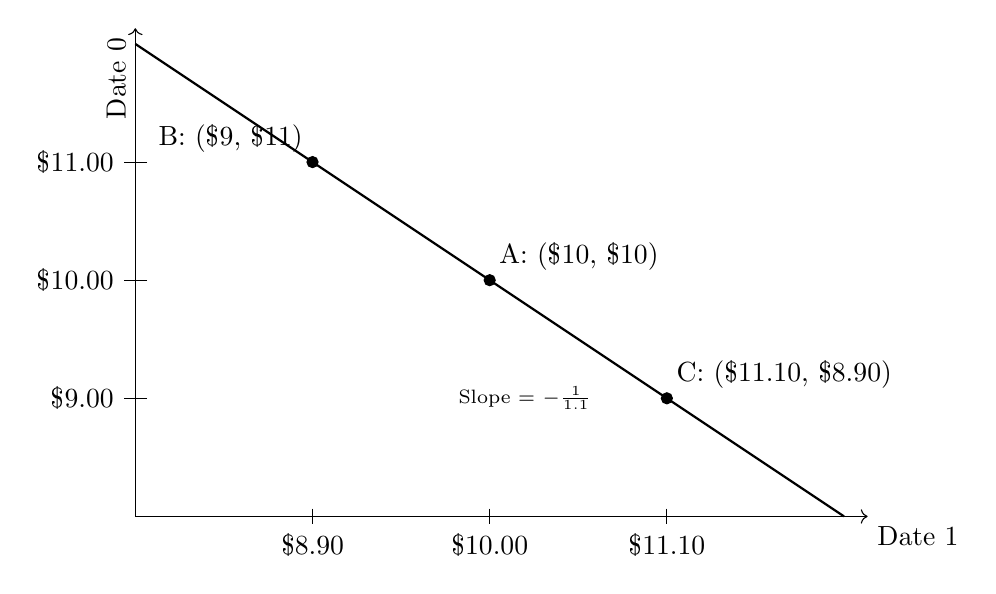
\begin{tikzpicture}[x=1.5cm, y=1cm]
    % Axes
    \draw[->] (0,0) -- (6.2,0) node[below right] {Date 1};
    \draw[->] (0,0) -- (0,6.2) node[above left, rotate=90] {Date 0};

    % Budget constraint line
    \draw[thick] (0,6) -- (6,0);

    % Key points
    \filldraw (3,3) circle (2pt) node[above right] {A: (\$10, \$10)};
    \filldraw (4.5,1.5) circle (2pt) node[above right] {C: (\$11.10, \$8.90)};
    \filldraw (1.5,4.5) circle (2pt) node[above left] {B: (\$9, \$11)};
    
    % Slope annotation
    \node at (3.3,1.5) {\scriptsize Slope = $-\frac{1}{1.1}$};

    % Ticks and labels
    \foreach \x/\xlabel in {1.5/\$8.90, 3/\$10.00, 4.5/\$11.10} {
        \draw (\x,0.1) -- (\x,-0.1) node[below] {\xlabel};
    }
    \foreach \y/\ylabel in {1.5/\$9.00, 3/\$10.00, 4.5/\$11.00} {
        \draw (0.1,\y) -- (-0.1,\y) node[left] {\ylabel};
    }

\end{tikzpicture}
}
\end{center}

\begin{itemize}
    \item Investors can freely move along the \textbf{budget line} by buying or selling shares to adjust the timing of cash flows.
    \item Point A: Firm policy $\rightarrow$ \$10 now and \$10 later.
    \item Point C: Preference for more cash now, offset by lower future income.
\end{itemize}

\end{frame}

\subsubsection*{Cash Dividend Summary}
\begin{frame}{Dividends and Investment Policy: Key Insight}

\begin{itemize}
    \item Increasing dividends by issuing new equity \textbf{does not create value} for shareholders.
    
    \item Reducing dividends through share repurchases \textbf{also does not destroy value}, assuming no change in total cash flow.

    \vspace{3mm}
    \item \textbf{Core Assumption:}
    \begin{itemize}
        \item The firm's overall cash flow level is fixed.
        \item The firm continues to accept all available \textbf{positive NPV projects}.
    \end{itemize}

    \vspace{3mm}
    \item \textbf{Golden Rule:}
    \begin{block}{}
        \centering
        \textit{A firm should never sacrifice a positive NPV investment just to increase or initiate a dividend.}
    \end{block}
\end{itemize}

\end{frame}

\subsection{Repurchase of Stock}
\begin{frame}{Repurchase of Stock: An Alternative to Dividends}

\begin{itemize}
    \item Instead of paying cash dividends, firms may choose to return excess cash via \textbf{share repurchases}.
    \item In a repurchase, the firm buys back its own shares, reducing the number of shares outstanding.
    
    \vspace{2mm}
    \item \textbf{Methods of Share Repurchase}:
    \begin{itemize}
        \item \textit{Open Market Repurchase}: Buy shares on the market like any investor.
        \item \textit{Tender Offer}: Offer to buy a specific number of shares at a premium.
        \item \textit{Dutch Auction}: Shareholders state prices; firm accepts the lowest prices that fulfill its target.
        \item \textit{Private Negotiation} (Greenmail): Buy back from large investors under negotiated terms.
    \end{itemize}
\end{itemize}

\end{frame}

\begin{frame}{Earnings, Dividends, and Buybacks for Large U.S. Firms}

\begin{figure}
    \centering
    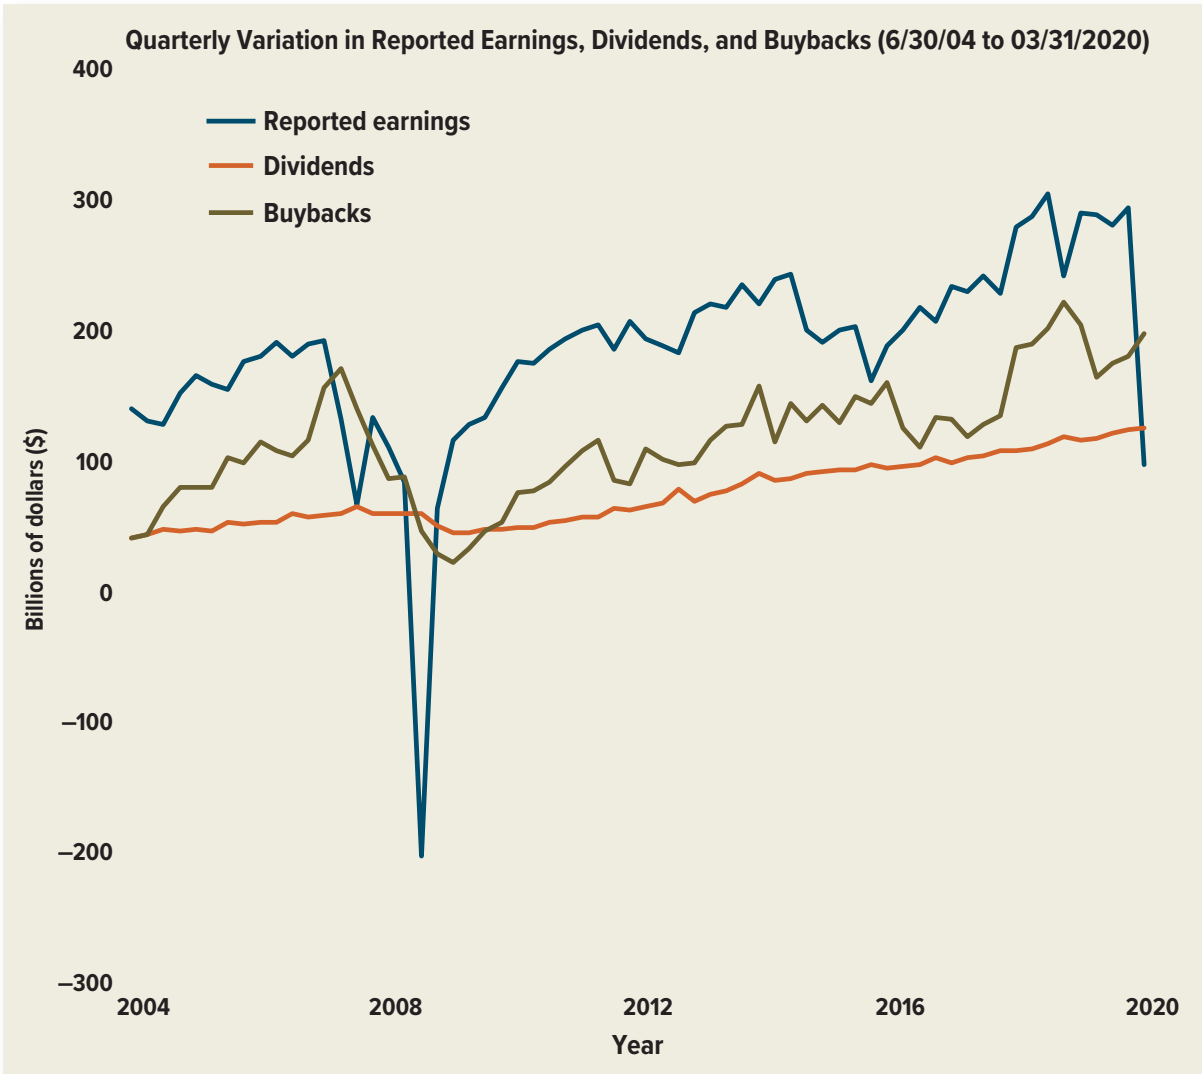
\includegraphics[width=0.6\textwidth]{images/section5/eds}
\end{figure}

\tiny{Source: Federal Reserve, via CFA Institute (through 03/31/2020)}

\end{frame}
\begin{frame}{Dividend vs. Stock Repurchase}{Original Balance Sheet}
	Consider a firm that wishes to distribute \$100,000 to its shareholders.
% Please add the following required packages to your document preamble:
% \usepackage{booktabs}
\begin{table}[]
	\begin{tabular}{@{}lrlr@{}}
		\multicolumn{2}{l}{\textit{\textbf{Assets}}} & \multicolumn{2}{l}{\textit{\textbf{Liabilities   \& Equity}}} \\
		\multicolumn{2}{l}{A. Original   balance sheet} &  & \multicolumn{1}{l}{} \\ \midrule
		Cash & \multicolumn{1}{r|}{\$150,000} & Debt & 0 \\
		Other Assets & \multicolumn{1}{r|}{\$850,000} & Equity & \$1,000,000 \\
		Value of Firm & \multicolumn{1}{r|}{\$1,000,000} & Value of Firm & \$1,000,000 \\ \bottomrule
	\end{tabular}
\end{table}
\begin{itemize}
	\item Shares outstanding = 100,000
	\item Price per share = \$1,000,000 / 100,000 = \$10
\end{itemize}
\end{frame}

\begin{frame}{Dividend vs. Stock Repurchase}{After Dividend Payment (Stock Price Falls)}
	If they distribute the \$100,000 as a cash dividend, the balance sheet will look like this:
	% Please add the following required packages to your document preamble:
	% \usepackage{booktabs}
	\begin{table}[]
		\begin{tabular}{@{}lrlr@{}}
			\multicolumn{2}{l}{\textit{\textbf{Assets}}} & \multicolumn{2}{l}{\textit{\textbf{Liabilities   \& Equity}}} \\
			\multicolumn{2}{l}{B. After \$1 per share cash dividend} &  & \multicolumn{1}{l}{} \\ \midrule
			Cash & \multicolumn{1}{r|}{\$50,000} & Debt & 0 \\
			Other Assets & \multicolumn{1}{r|}{\$850,000} & Equity & \$900,000 \\
			Value of firm & \multicolumn{1}{r|}{\$900,000} & Value of firm & \$900,000 \\ \bottomrule
		\end{tabular}
	\end{table}
\begin{itemize}
\item Shares outstanding = 100,000
\item Price per share = \$900,000 / 100,000 = \$9
\end{itemize}
\end{frame}

\begin{frame}{Dividend vs. Stock Repurchase}{After Stock Repurchase (Stock Price Stable, Shares Reduce)}
If they distribute the \$100,000 through a stock repurchase, the balance sheet will look like this:
% Please add the following required packages to your document preamble:
% \usepackage{booktabs}
\begin{table}[]
	\begin{tabular}{@{}lrlr@{}}
		\multicolumn{2}{l}{\textit{\textbf{Assets}}} & \multicolumn{2}{l}{\textit{\textbf{Liabilities   \& Equity}}} \\
		\multicolumn{2}{l}{C.  After stock repurchase} &  & \multicolumn{1}{l}{} \\ \midrule
		Cash & \multicolumn{1}{r|}{\$50,000} & Debt & 0 \\
		Other Assets & \multicolumn{1}{r|}{\$850,000} & Equity & \$900,000 \\
		Value of firm & \multicolumn{1}{r|}{\$900,000} & Value of firm & \$900,000 \\ \bottomrule
	\end{tabular}
\end{table}
\begin{itemize}
	\item Shares outstanding = 90,000
	\item Price per share = \$900,000 / 90,000 = \$10
\end{itemize}
\end{frame}
\begin{frame}{Dividend vs. Repurchase: Key Insight}

\begin{itemize}
    \item In a perfect market (no taxes, transaction costs, or signaling effects), \textbf{dividends and repurchases are equivalent}.
    \item Key difference:
    \begin{itemize}
        \item \textbf{Dividends} reduce cash and equity; share price falls.
        \item \textbf{Repurchases} reduce cash and shares; share price stays the same.
    \end{itemize}
    \item Choice between them depends on taxes, signaling, flexibility, and incentives.
\end{itemize}

\end{frame}

\begin{frame}{Why Do Firms Prefer Repurchases?}

\textbf{1. Flexibility}
\begin{itemize}
    \item Dividends are viewed as commitments; cuts are penalized.
    \item Repurchases offer temporary, non-binding payouts.
\end{itemize}

\vspace{2mm}
\textbf{2. Managerial Incentives}
\begin{itemize}
    \item Repurchases increase EPS and stock price -- both favorable to option-holding executives.
    \item Firms use repurchases to offset dilution from equity compensation.
\end{itemize}

\end{frame}

\begin{frame}{Why Do Firms Prefer Repurchases? (cont'd)}

\textbf{3. Signaling}
\begin{itemize}
    \item Repurchase announcements often interpreted as \textit{"we believe our stock is undervalued"}.
\end{itemize}

\vspace{2mm}
\textbf{4. Tax Efficiency}
\begin{itemize}
    \item Capital gains from repurchases are taxed more favorably than dividends in many jurisdictions.
\end{itemize}

\vspace{2mm}
\textbf{5. Takeover Defense}
\begin{itemize}
    \item Repurchases reduce shares available to potential hostile acquirers.
\end{itemize}

\end{frame}

\begin{frame}{Summary: Dividend vs. Share Repurchase}

\begin{table}[ht]
\centering
\resizebox{\linewidth}{!}{
\begin{tabular}{l >{\raggedright\arraybackslash}p{4.5cm} >{\raggedright\arraybackslash}p{6.5cm}}
\toprule
\textbf{Dimension} & \textbf{Dividends} & \textbf{Share Repurchases} \\
\midrule
\textbf{Flexibility} & Typically viewed as a long-term commitment & More flexible, can be adjusted based on cash flows \\
\textbf{Signal to Market} & May signal confidence if increased & Often viewed as a signal of undervaluation \\
\textbf{Tax Treatment} & Taxed as dividend income (often higher) & Taxed as capital gains (usually lower) \\
\textbf{Effect on Share Price} & Share price drops on ex-dividend date & Share price often unchanged, but EPS increases \\
\textbf{Impact on Share Count} & No change in shares outstanding & Reduces shares outstanding, increases ownership concentration \\
\textbf{Effect on Management Incentives} & Less direct impact on stock options & May increase value of outstanding stock options \\
\bottomrule
\end{tabular}
}
\end{table}

\end{frame}

\subsection{Personal Taxes and Payout Policy}
\begin{frame}{Personal Taxes and Payout Policy}
    \begin{itemize}
        \item The irrelevance of dividend policy relies on idealized assumptions:
        \begin{itemize}
            \item No taxes
            \item No transaction costs
            \item No uncertainty
        \end{itemize}
        \item In practice, taxes introduce important frictions:
        \begin{itemize}
            \item In \textbf{China}:
            \begin{itemize}
                \item Cash dividends are taxed at \textbf{20\%}.
                \item Capital gains tax exists but is not always enforced.
            \end{itemize}
            \item In the \textbf{U.S.}:
            \begin{itemize}
                \item Both dividends and capital gains are taxed at \textbf{15\%}.
                \item \textit{Capital gains are deferrable}—effective tax rate is lower.
            \end{itemize}
        \end{itemize}
        \item Bottom line: \textbf{Dividends are typically taxed more heavily than capital gains}.
    \end{itemize}
\end{frame}

\begin{frame}{Payouts with No Taxes}
    \begin{itemize}
        \item Suppose a firm distributes dividends but lacks sufficient cash.
        \item The firm raises funds via stock issuance and returns those funds as dividends.
        \item \textbf{Result:} A complete wash -- no change in shareholder wealth.
    \end{itemize}
    \begin{figure}
        \centering
        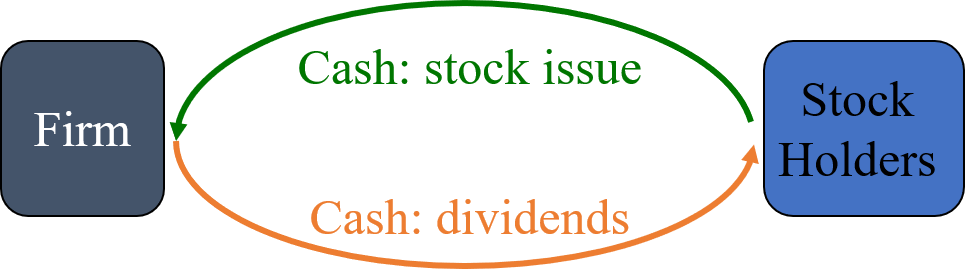
\includegraphics[width=0.65\textwidth]{images/section5/firmwithout1.png}
    \end{figure}
\end{frame}

\begin{frame}{Payouts with Taxes: Destroying Value}
    \begin{itemize}
        \item Now assume a \textbf{15\% tax} on dividends.
        \item Issuing shares to pay dividends incurs a tax burden on shareholders.
        \item \textbf{Conclusion:} This strategy reduces overall value and is dominated by doing nothing.
    \end{itemize}
    \begin{figure}
        \centering
        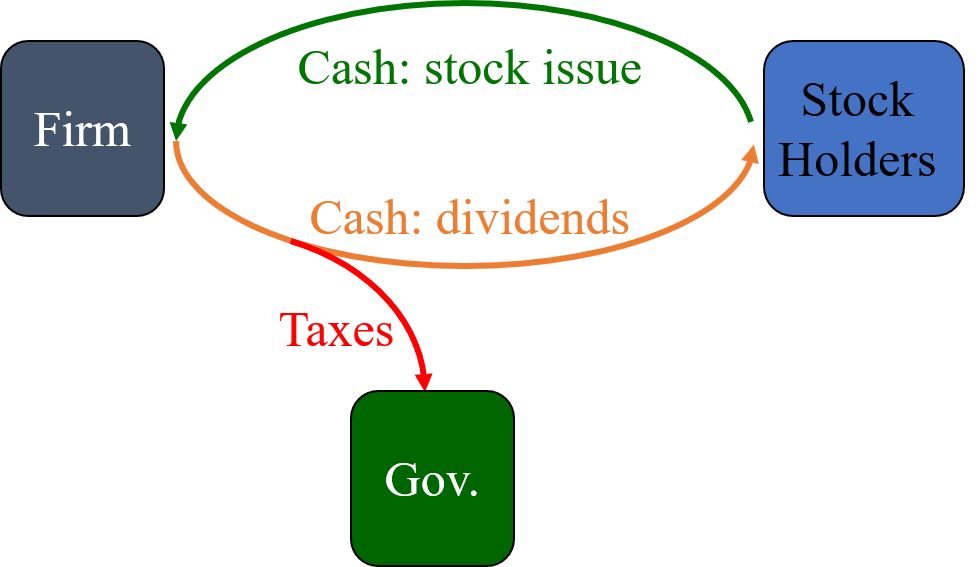
\includegraphics[width=0.65\textwidth]{images/section5/firmwithout2.png}
    \end{figure}
\end{frame}

\begin{frame}{Payouts with Taxes + Transaction Costs}
    \begin{itemize}
        \item In addition to tax inefficiency, \textbf{stock issuance incurs fees}.
        % \item Investment banks and legal expenses reduce the firm's remaining value.
        % \item \textbf{Lesson:} Never issue equity just to pay dividends.
    \end{itemize}
    \begin{figure}
        \centering
        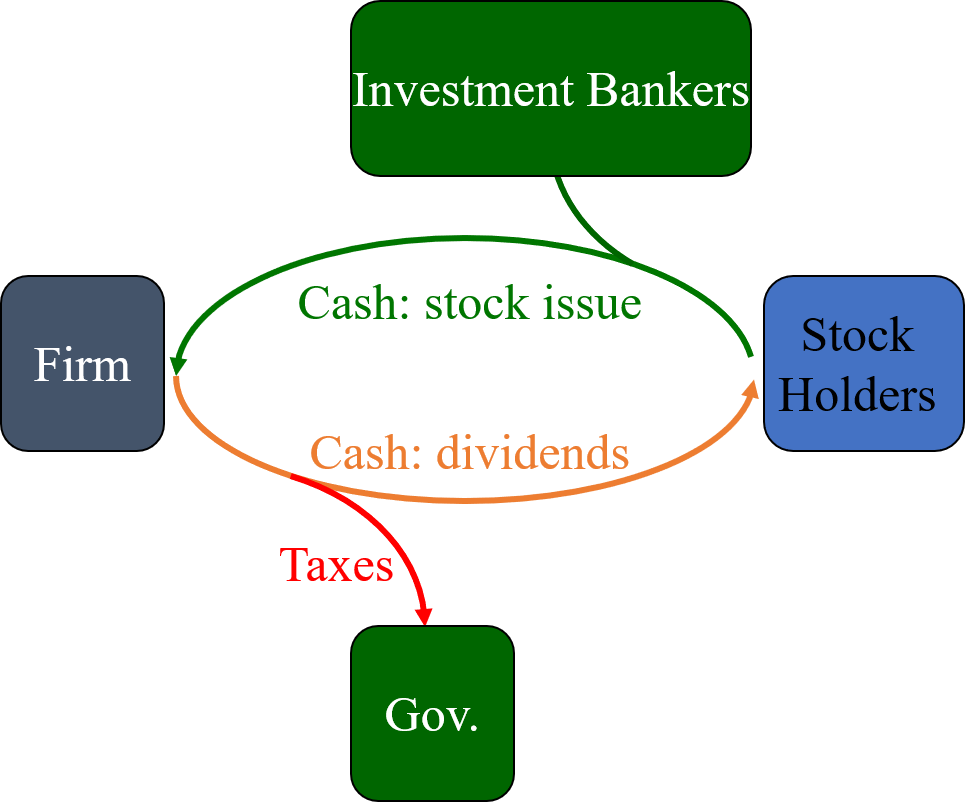
\includegraphics[width=0.65\textwidth]{images/section5/firmwithout3.png}
    \end{figure}
\end{frame}

\begin{frame}{When Firms Have Excess Cash}
    \begin{itemize}
        \item Tax arguments apply differently when the firm has extra cash \textbf{after investing in all positive NPV projects}.
        \item Options for excess funds:
        \begin{itemize}
            \item Take on negative NPV projects (value destroying)
            \item Acquire firms or buy financial assets
            \item Distribute cash via \textbf{dividends or share repurchases}
        \end{itemize}
        \item \textbf{Best practice:} return excess capital to shareholders unless a superior use exists.
    \end{itemize}
\end{frame}
\begin{frame}{Dividend Timing and Tax Efficiency}
    \begin{block}{Example: Regional Electric Company}
        Regional Electric has \$1,000 of excess cash. It can either:
        \begin{enumerate}
            \item Pay the amount as a \textbf{dividend now}, or
            \item \textbf{Retain and invest} it in 10\% Treasury bills, paying a dividend after 5 years.
        \end{enumerate}
        \vspace{0.2cm}
        \textbf{Assumptions:}
        \begin{itemize}
            \item Corporate tax rate: 21\%
            \item Personal tax rate on interest: 28\%
            \item Dividend tax rate: 15\%
            \item Investors can also invest in 10\% Treasury bills directly
        \end{itemize}
        \textbf{Question:} Which policy leaves investors better off after 5 years?
    \end{block}
\end{frame}
\begin{frame}{After-Tax Wealth: Immediate vs Deferred Dividend}
    \begin{itemize}
        \item \textbf{Option 1: Pay dividend now}
        \begin{itemize}
            \item Dividend received: \$1,000 × (1 - 15\%) = \$850
            \item Invest at 10\% for 5 years, taxed at 28\%:
            \[
            \$850 \times \left[1 + 0.10 \times (1 - 0.28)\right]^5 = \text{\$1,203.35}
            \]
        \end{itemize}

        \vspace{0.3cm}
        \item \textbf{Option 2: Retain cash, invest in T-bills, pay dividend in Year 5}
        \begin{itemize}
            \item Corporate investment grows at after-tax return:
            \[
            \$1,000 \times \left[1 + 0.10 \times (1 - 0.21)\right]^5 = \text{\$1,462.54}
            \]
            \item Dividend taxed at 15\% in Year 5:
            \[
            \$1,462.54 \times (1 - 0.15) = \text{\$1,243.16}
            \]
        \end{itemize}

        \vspace{0.3cm}
        \item \textbf{Conclusion:} Deferring the dividend results in greater after-tax wealth:  
        \textbf{\$1,243.16 vs. \$1,203.35}
    \end{itemize}
\end{frame}

\begin{frame}{Summary: Personal Taxes and Payout Policy}
	\begin{itemize}
		\item \textbf{In a world with personal taxes:}
		\begin{itemize}
			\item Firms should \textbf{not issue equity to pay dividends} -- this is inefficient due to double taxation.
			\item Managers have incentives to minimize dividend payments by seeking alternative uses for cash:
			\begin{itemize}
				\item Invest in capital expenditures (CAPEX)
				\item Pursue M\&A opportunities
				\item Accumulate financial assets (e.g., T-bills)
			\end{itemize}
			\item However, \textbf{practical limits} on these activities often leave firms with excess cash -- resulting in residual dividend payments.
		\end{itemize}
		\vspace{0.2cm}
		\item \textbf{Key tension:}  
		Personal taxes reduce the attractiveness of dividends, yet most firms continue to pay them.
		
		\item \textbf{Open puzzle:}  
		Why do firms \textit{prefer dividends} over tax-efficient share repurchases?
	\end{itemize}
\end{frame}

\subsection{Real-World Factors Favoring High Dividends}
\begin{frame}{Why Firms Might Favor High Dividends}
	\begin{itemize}
		\item \textbf{Investor Preference for Current Income} -- Especially retirees or income-focused investors.
		\item \textbf{Behavioral Factors} -- Dividends act as a self-control device for spending.
		\item \textbf{Agency Costs} -- Paying dividends reduces managerial discretion over free cash flow.
		\item \textbf{Information Content and Signaling} -- Dividend changes convey management's private information.
	\end{itemize}
\end{frame}

\subsubsection{Investor Preference, Behavioral Finance and Clientele Effect}
\begin{frame}{Investor Preference for Current Income}
\footnotesize
\begin{itemize}
    \item \textbf{Some investors -- particularly retirees -- prioritize stable cash flows} to fund consumption without selling shares.

    \item \textbf{In theory}: With no taxes or frictions, dividends and share sales are equivalent -- investors could create "homemade dividends."

    \item \textbf{In practice}:
    \begin{itemize}
        \item Selling shares involves \textit{transaction costs}, \textit{capital gains taxes}, and \textit{timing risk}.
        \item Dividends offer convenience, simplicity, and predictable cash flow.
    \end{itemize}

    \item \textbf{Conclusion:} Demand for dividends from income-oriented investors may push up the prices of high-dividend stocks.
\end{itemize}
\end{frame}

\begin{frame}{Behavioral Finance: Self-Control and Dividend Demand}
\footnotesize
\begin{itemize}
    \item \textbf{Self-control problems} can lead investors to overconsume or mismanage withdrawals from investments.

    \item Two strategies to generate income:
    \begin{itemize}
        \item \textbf{Dividend discipline:} Consume only what is paid as dividends -- automatic budgeting.
        \item \textbf{Self-liquidation:} Sell shares as needed -- requires restraint and active decision-making.
    \end{itemize}

    \item \textbf{Behavioral insight:} Regular dividends act as a commitment device, helping avoid temptation and poor timing.

    \item \textbf{Implication:} Even if inefficient in theory, dividends may enhance welfare by supporting investor discipline.
\end{itemize}
\end{frame}

\begin{frame}{From Self-Control to Clientele Effects}
\footnotesize
\begin{itemize}
    \item \textbf{Behavioral motivations, like self-control, help explain why some investors prefer dividends.}
    
    \item But dividend demand isn't driven by behavior alone.
    \begin{itemize}
        \item Taxes, income needs, and institutional constraints also play a role.
    \end{itemize}
    
    \vspace{0.2cm}
    \item \textbf{Together, these factors form the basis of the \textit{Dividend Clientele Hypothesis}}:
    \begin{itemize}
        \item Different investor groups prefer different payout policies.
        \item Firms may shape or respond to the makeup of their shareholder base accordingly.
    \end{itemize}
    
    \vspace{0.2cm}
    \item \textbf{Next:} We explore who prefers what -- and why -- in dividend clientele formation.
\end{itemize}
\end{frame}

\begin{frame}{The Dividend Clientele Effect}
\footnotesize
\begin{itemize}
    \item \textbf{Investor preferences vary by tax status and income needs} -- creating distinct "clienteles" for dividend policies.
\end{itemize}

\vspace{0.2cm}
\begin{table}[h]
	\centering
	\small
    \begin{tabular}{ll}
		\toprule
		\textbf{Investor Group} & \textbf{Preferred Payout Policy} \\
		\midrule
		High-Tax Individuals & Low or No Dividends \\
		Retirees / Income-Seekers & Moderate to High Dividends \\
		Tax-Exempt Institutions & Indifferent or High Dividends \\
		Corporations & High Dividends (due to inter-corporate exemption) \\
		\bottomrule
	\end{tabular}
	
\end{table}

\vspace{0.2cm}
\begin{itemize}
    \item \textbf{Implication:} Firms may tailor payout policy to attract or retain their target shareholder base.
\end{itemize}
\end{frame}

\begin{frame}{Retail Investor Preferences: Empirical Evidence}
\footnotesize
\begin{itemize}
    \item Surveys and trading data show that \textbf{many individual investors prefer high-dividend stocks}.
    \item This preference persists despite theoretical arguments for dividend irrelevance.
\end{itemize}

\begin{figure}
    \centering
    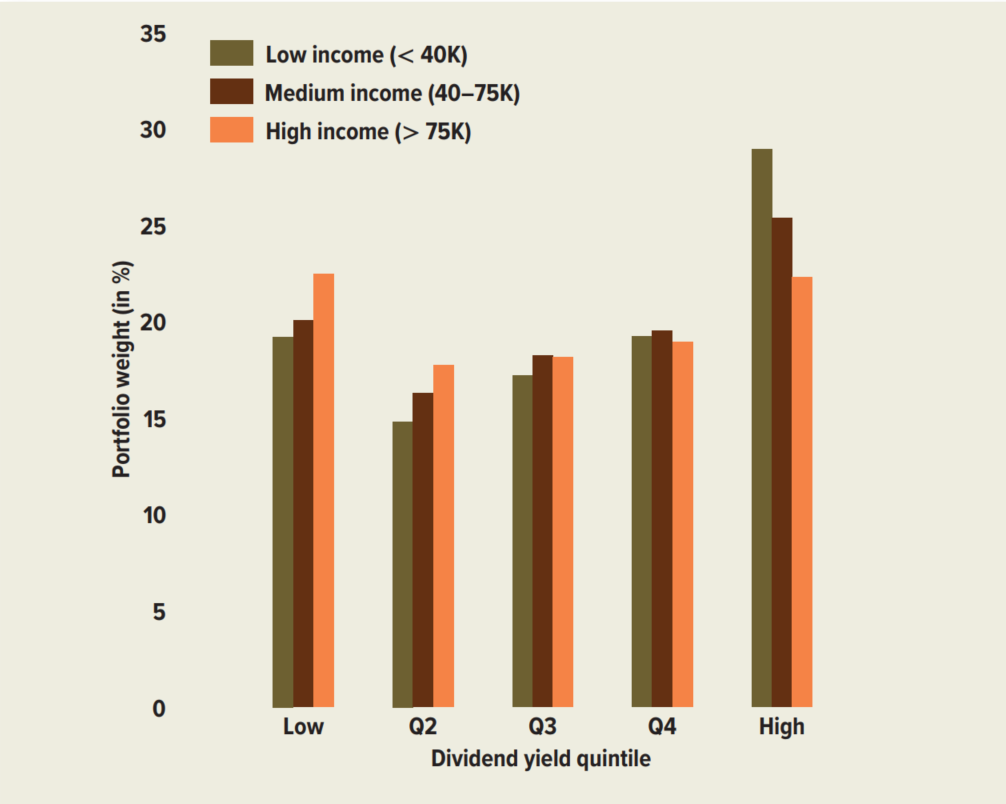
\includegraphics[height=0.5\textheight]{images/section5/dividendyield}
\end{figure}

\tiny{Source: \textcite{graham2006dividend}. Retail investors reveal a bias toward high dividend yields in portfolio choices.}
\end{frame}

\begin{frame}{Summary: Behavioral and Clientele Effects}
\begin{figure}
    \centering
    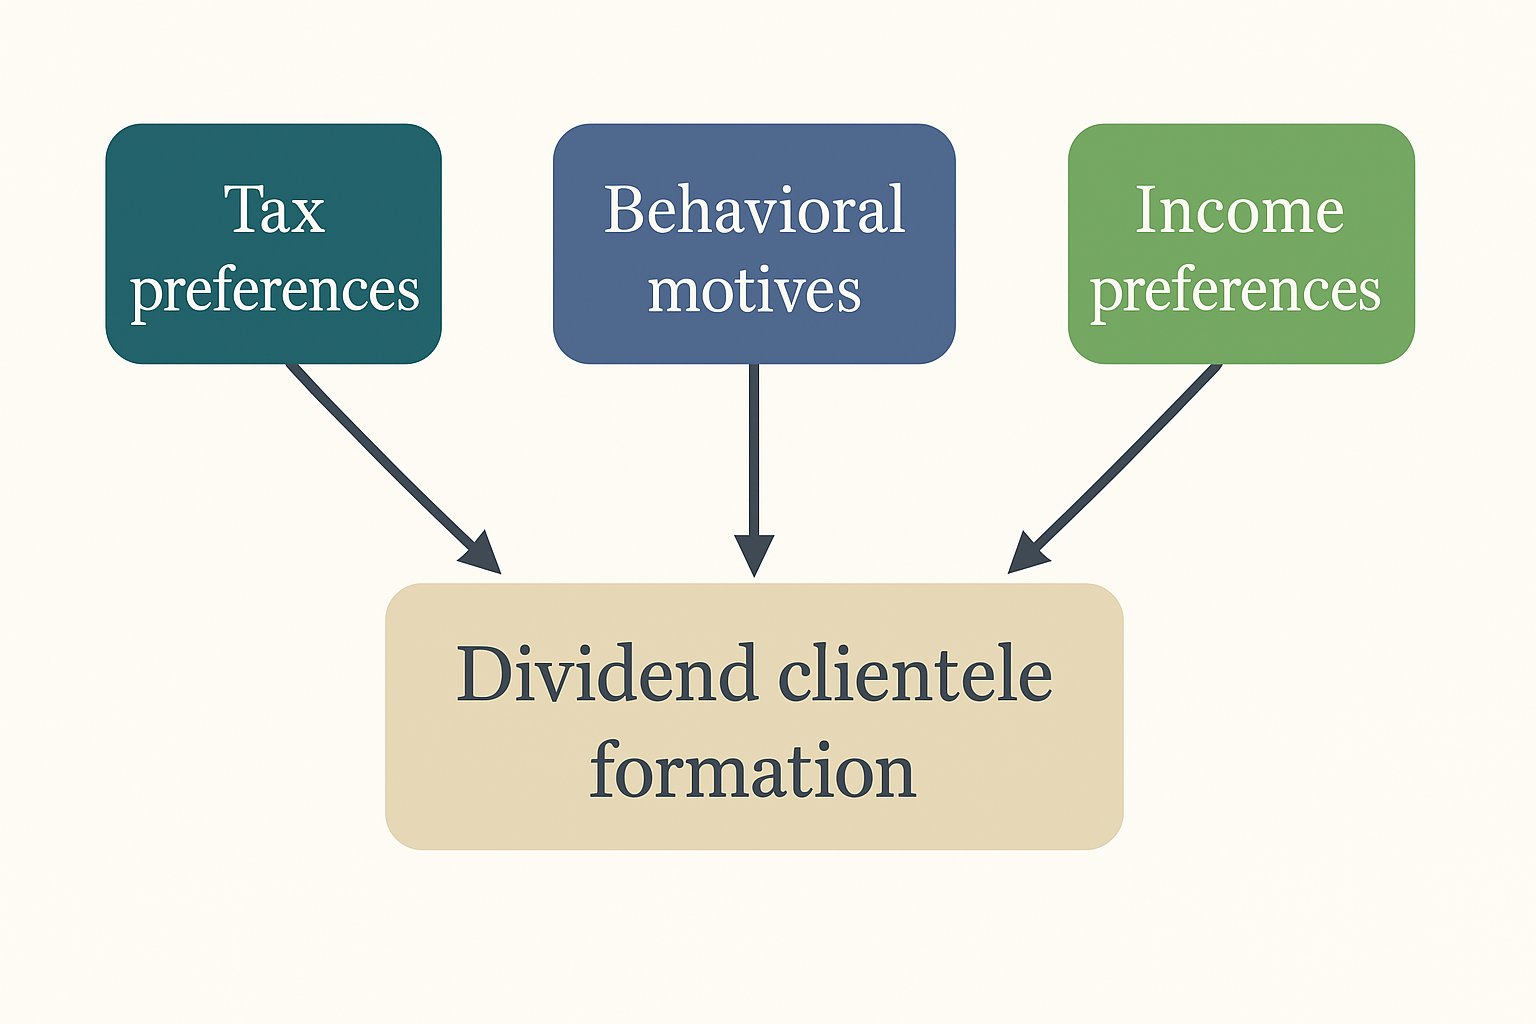
\includegraphics[width=0.8\linewidth]{images/section5/clientele.png}
\end{figure}
\end{frame}

\subsubsection{Dividends and Agency Costs}
\begin{frame}{Dividends and Agency Costs}
\footnotesize
\begin{itemize}
    \item \textbf{Agency Conflict:} Managers may pursue inefficient investments, perks, or empire-building when excess cash is available.
    
    \vspace{1mm}
    \item \textbf{Role of Dividends:}
    \begin{itemize}
        \item Reduces \textbf{free cash flow} under managerial discretion.
        \item Forces managers to return capital to shareholders rather than reinvest wastefully.
    \end{itemize}
    
    \vspace{1mm}
    \item \textbf{Additional Effects:}
    \begin{itemize}
        \item May \textit{transfer wealth from bondholders to shareholders} during financial distress.
        \item Acts as a \textbf{signal} that management prioritizes shareholder interests.
    \end{itemize}
    
    \vspace{1mm}
    \item \textbf{Implication:} Dividend policy can serve as a governance mechanism in firms with high free cash flow.
\end{itemize}
\end{frame}

\subsubsection{Information Content of Dividends and Dividend Signaling}

\begin{frame}{Information Content of Dividends}
\footnotesize
\begin{itemize}
    \item Dividend changes convey management's private information about future performance:
    \begin{itemize}
        \item \textbf{Increase} $\rightarrow$ signal of expected stronger future cash flows and earnings
        \item \textbf{Decrease} $\rightarrow$ often interpreted as a sign of financial weakness
    \end{itemize}

    \vspace{2mm}
    \item Academic evidence supports this view:
    \begin{itemize}
        \item \textcite{asquith1983impact} and \textcite{michaely1995price} show positive abnormal returns following dividend increases, and negative returns after cuts.
    \end{itemize}

    \item \textbf{Takeaway:} The stock market reacts not just to the amount of dividends, but to the information embedded in changes to dividend policy.
\end{itemize}
\end{frame}

\begin{frame}{Dividend Signaling: Why It's Credible}
\footnotesize
\begin{itemize}
    \item \textbf{Can firms "fake" strong performance by raising dividends?}
    \begin{itemize}
        \item In the short term, yes -- but only at a cost.
        \item Higher dividends must be paid in cash -- real money, not just promises.
    \end{itemize}

    \vspace{2mm}
    \item \textbf{Why is the signal credible?}
    \begin{itemize}
        \item Firms with weak earnings cannot sustain elevated payouts without jeopardizing liquidity or future investment.
        \item This cost makes it unattractive for low-quality firms to mimic high-quality ones.
    \end{itemize}

    \vspace{2mm}
    \item \textbf{Implication:} Only firms with strong future prospects raise dividends, making dividend increases a \textbf{credible signal}.
\end{itemize}
\end{frame}

\begin{frame}{Dividend Announcement and Market Inference (I)}
\footnotesize
\textbf{Assumption:}  
Firm is all-equity financed. Identity:
\[
\text{Cash Flow} = \text{CapEx} + \text{Dividends}
\]

\vspace{2mm}
\textbf{Scenario A:}
\begin{itemize}
    \item Firm announces CapEx = \$80 million
    \item Market believes Cash Flow = \$130 million
    \item $\Rightarrow$ Market infers Dividend = \$50 million
\end{itemize}

\vspace{2mm}
\textbf{Scenario B:}
\begin{itemize}
    \item Firm announces Dividend = \$70 million (higher than expected)
    \item Market assumes Cash Flow unchanged (\$130M) $\rightarrow$ CapEx = \$60M
    \item Market reacts negatively $\rightarrow$ assumes profitable investment opportunities are being sacrificed
\end{itemize}
\end{frame}

\begin{frame}{Dividend Announcement and Market Inference (II)}
\footnotesize
\textbf{Alternative Market Interpretation:}
\begin{itemize}
    \item CapEx = \$80M remains unchanged
    \item Dividend = \$70M implies Cash Flow = \$150M
    \item Market revises expectations upward $\rightarrow$ stock price rises
\end{itemize}

\vspace{2mm}
\textbf{Credibility Mechanism:}
\begin{itemize}
    \item If firm raises dividends but doesn't have the cash flow, it will have to cut CapEx or raise funds.
    \item The truth will eventually be revealed through realized cash flows.
    \item Hence, only firms with sustainable earnings can afford to send this signal.
\end{itemize}

\vspace{2mm}
\textbf{Conclusion:}  
Dividend increases are costly to fake $\rightarrow$ they function as a \textbf{credible and informative signal} of firm strength.
\end{frame}

\subsubsection*{Summary}
\begin{frame}{Summary: Real-World Drivers of High Dividend Policy}
\footnotesize
\begin{itemize}
    \item \textbf{Investor Preferences}
    \begin{itemize}
        \item Some investors (e.g., retirees) desire stable income $\rightarrow$ prefer dividend-paying stocks.
        \item Transaction costs, taxes, and behavioral self-control make dividends more appealing than homemade alternatives.
        \item \textit{Clientele effect:} Different groups prefer different payout policies -- firms may cater to them.
    \end{itemize}
    \item \textbf{Agency Considerations}
    \begin{itemize}
        \item Dividends reduce free cash flow, limiting managerial discretion and curbing inefficiencies.
        \item May shift value from bondholders to shareholders during distress.
    \end{itemize}
    \item \textbf{Information and Signaling}
    \begin{itemize}
        \item Dividend increases can signal future profitability.
        \item Signaling is \textbf{costly to fake} -- only high-quality firms can sustain higher payouts.
    \end{itemize}
    % \item \textbf{Takeaway:}  
    % Though dividends may appear irrelevant in theory, real-world frictions make them a powerful corporate policy tool.
\end{itemize}
\end{frame}

\subsection{How Firms Pay Dividends Today}
\begin{frame}{How Firms Pay Dividends Today: Global Trends and Stylized Facts}
\footnotesize
\begin{itemize}
    \item \textbf{Dividends remain central to corporate payouts} despite theories of irrelevance.
    \begin{itemize}
        \item Aggregate global payouts continue to rise -- surpassing \$1.7 trillion in 2024.
        \item But the share of dividend-paying firms has declined in developed markets like the U.S.
    \end{itemize}
    \item \textbf{Corporate payout behavior is shaped by three regularities:}
    \begin{itemize}
        \item Firms \textit{smooth dividends} over time and avoid cuts.
        \item Dividends reflect long-term commitment; repurchases offer short-term flexibility.
        \item Payout policy adapts to firm characteristics, market norms, and investor demand.
    \end{itemize}
    \item \textbf{Cross-country variation matters.}
    \begin{itemize}
        \item Tax policies, institutional ownership, and governance norms shape dividend behavior.
        \item \textit{China's evolving payout practices} offer a revealing contrast to Western models.
    \end{itemize}
\end{itemize}
\end{frame}


\begin{frame}{Dividends Remain Substantial in Practice}
\footnotesize
\begin{itemize}
    \item \textbf{Despite theoretical arguments for dividend irrelevance, aggregate dividend payouts have grown steadily over time.}
    
    \vspace{2mm}
    \item \textbf{Key evidence:}
    \begin{itemize}
        \item In the U.S., total dividends paid by listed firms more than tripled from the 1980s to the 2020s.
        \item Globally, dividends constitute a significant share of total equity returns.
    \end{itemize}
    
    \vspace{2mm}
    \item \textbf{Reasons dividends remain relevant:}
    \begin{itemize}
        \item Institutional investor demand (e.g., pension funds)
        \item Cultural and market expectations
        \item Managerial incentives tied to dividend performance
    \end{itemize}
\end{itemize}
\end{frame}

\begin{frame}{Global Dividend Payouts Reach Record \$1.75 Trillion in 2024}
% \footnotesize
% \begin{itemize}
%     \item Despite the rise of share repurchases and shifting investor preferences, global dividend payouts remain at record highs.
    
%     \item \textbf{In 2024, global dividends reached \$1.75 trillion}, driven by robust corporate profits and continued shareholder demand for income.
    
%     \item The chart (right) shows the steady upward trend in total global dividends over the past 15 years -- with notable resilience even during periods of global uncertainty (e.g., COVID-19).
    
%     \item \textbf{Key features:}
%     \begin{itemize}
%         \item Both regular and special dividends have grown substantially.
%         \item The post-pandemic recovery saw a particularly strong rebound in payouts.
%     \end{itemize}

%     \item \textbf{Source:} Janus Henderson Global Dividend Index (2025)
% \end{itemize}

\begin{figure}
    \centering
    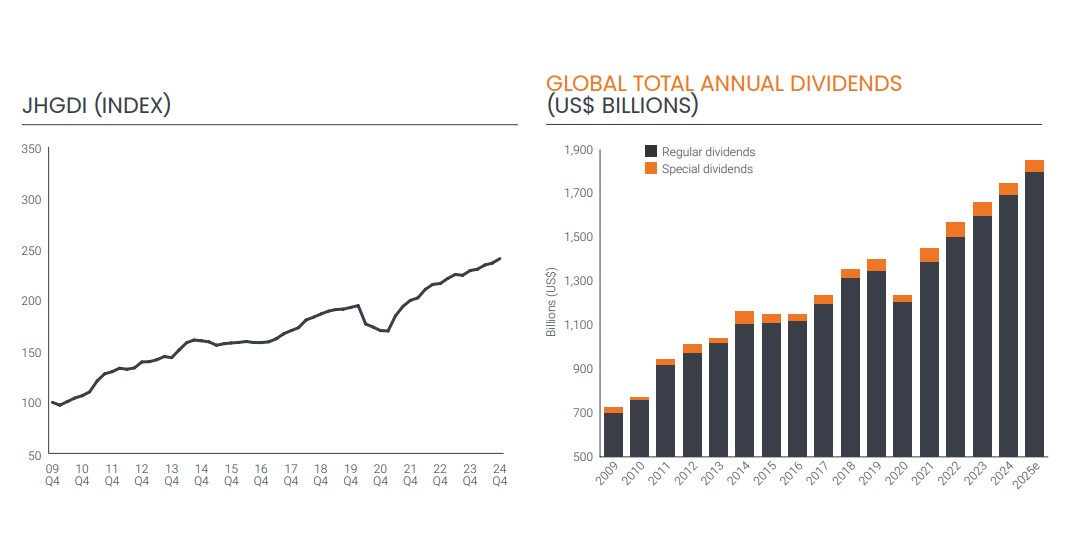
\includegraphics[width=0.85\linewidth]{images/section5/JHGDI.jpg}
\end{figure}
{\tiny
\textbf{Source:} Janus Henderson Global Dividend Index (2025) \url{https://www.fundssociety.com/en/news/markets/global-dividend-payouts-reach-record-1-75-trillion-in-2024/}}
\end{frame}

\begin{frame}{Dividends vs. Buybacks: S\&P 500 (1998-2020)}
\begin{figure}
    \centering
    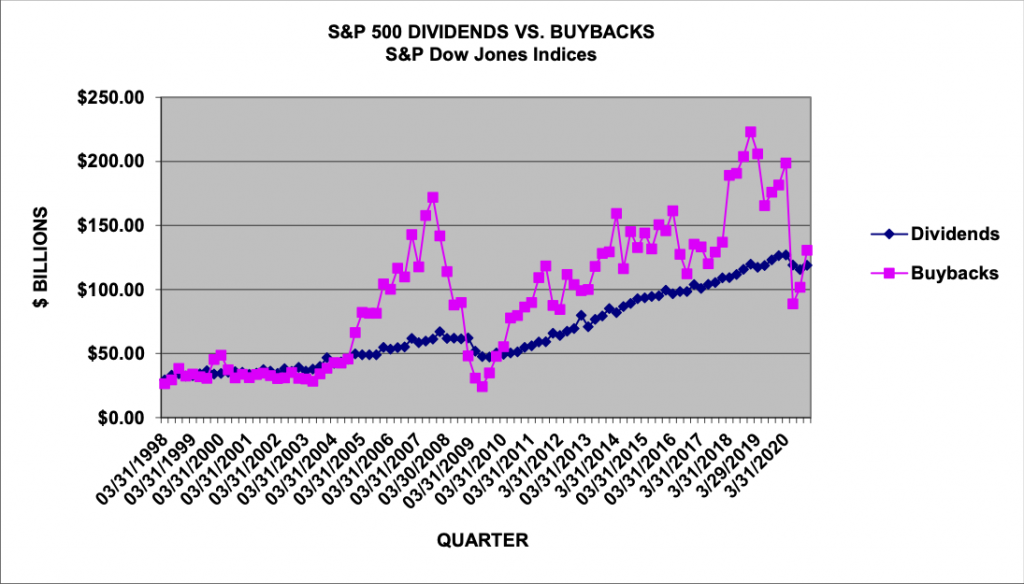
\includegraphics[width=0.95\linewidth]{images/section5/dividends_vs_buybacks.png}
\end{figure}
\tiny{Source: S\&P Dow Jones Indices. \url{https://dqydj.com/sp-500-dividend-yield/}}
\end{frame}

\begin{frame}{Trends in Corporate Payouts: Key Observations}
\footnotesize
\begin{itemize}
    \item \textbf{Both dividends and stock buybacks increased significantly} over the past two decades, but their patterns differ:
    \begin{itemize}
        \item Dividends grow steadily and predictably.
        \item Buybacks are more volatile -- firms ramp up repurchases during booms and cut them during downturns.
    \end{itemize}
    
    \vspace{2mm}
    \item \textbf{Since the mid-2000s, buybacks have often exceeded dividends}, indicating a shift in corporate payout preference.
    
    \vspace{2mm}
    \item \textbf{During economic shocks} (e.g., 2008 crisis, COVID-19 pandemic), companies generally preserve dividends but slash buybacks -- suggesting dividends are perceived as stronger signals of financial stability.
    
    \vspace{2mm}
    \item \textbf{Takeaway:} Dividends are viewed as long-term commitments; buybacks offer flexibility and are used more opportunistically.
\end{itemize}
\end{frame}

\begin{frame}{Dividend Smoothing: Lintner's Model}
\footnotesize
\begin{itemize}
    \item \textbf{\textcite{lintner1956distribution}} interviewed managers and found two consistent behaviors:
    \begin{itemize}
        \item Firms aim for a \textbf{target payout ratio} of earnings over the long run.
        \item Managers adjust dividends \textbf{gradually}, as they wait to confirm earnings changes are permanent.
    \end{itemize}

    \vspace{2mm}
    \item Dividend changes follow the adjustment model:
    \[
    D_1 - D_0 = s \times (t \cdot \text{EPS}_1 - D_0)
    \]
    where:
    \begin{itemize}
        \item $D_1$: dividend next year; $D_0$: dividend this year
        \item $t$: target payout ratio
        \item $s$: speed of adjustment ($0 < s \leq 1$)
    \end{itemize}

    \vspace{2mm}
    \item \textbf{Implication:} Dividend policy is \textit{sticky}, forward-looking, and resistant to transitory earnings fluctuations.
\end{itemize}
\end{frame}

\begin{frame}{Example: Applying Lintner's Smoothing Model}
\footnotesize
\begin{itemize}
    \item Calculator Graphics, Inc. (CGI) follows:
    \begin{itemize}
        \item Target payout ratio $t = 0.30$
        \item Speed of adjustment $s = 0.5$
    \end{itemize}

    \item \textbf{Year 1:}
    \begin{itemize}
        \item Last year's EPS = \$10, dividends = \$3.00
        \item This year's EPS = \$20
        \item Implied dividend change:
        \[
        \Delta D = 0.5 \times (0.30 \times 20 - 3.00) = 1.50
        \]
        \item New dividend = \$4.50
    \end{itemize}

    \item \textbf{Year 2:} EPS remains at \$20
    \begin{itemize}
        \item New target = \$6.00; current = \$4.50
        \item \[
        \Delta D = 0.5 \times (6.00 - 4.50) = 0.75
        \]
        \item New dividend = \$5.25
    \end{itemize}

    \item \textbf{Conclusion:} Dividend growth is \textit{deliberate and partial}, not a mechanical response to earnings.
\end{itemize}
\end{frame}

\begin{frame}{Chinese Firms: Rising Payouts and Policy Push}
\footnotesize
\begin{itemize}
    \item Chinese listed firms are increasing shareholder payouts under \textbf{regulatory pressure} and growing \textbf{investor demand for returns}.
    \item Reuters/LSEG data reported cash dividends by large and mid-cap Chinese companies reaching a record ¥3.4 trillion in 2023, with projected growth of 1.2\% in 2024 and 8.6\% in 2025.
    \begin{itemize}
        \item These figures cover a broad universe of Chinese-listed firms; A-share-only data may show different patterns.
    \end{itemize}
    \item \textbf{Key drivers:}
    \begin{itemize}
        \item \textit{Regulatory reform:} CSRC and SASAC have issued guidance encouraging stronger shareholder returns.
        \item \textit{Governance pressure:} Reducing idle cash improves capital discipline.
        \item \textit{Investor demand:} Income-seeking investors and dividend ETF flows reinforce the trend.
    \end{itemize}
    \item \textbf{Bottom line:} China's payout policy is increasingly shaped by policy reform, governance concerns, and investor-return pressure.
\end{itemize}
\end{frame}

\begin{frame}{Dividend Payout Trends in China}
\centering
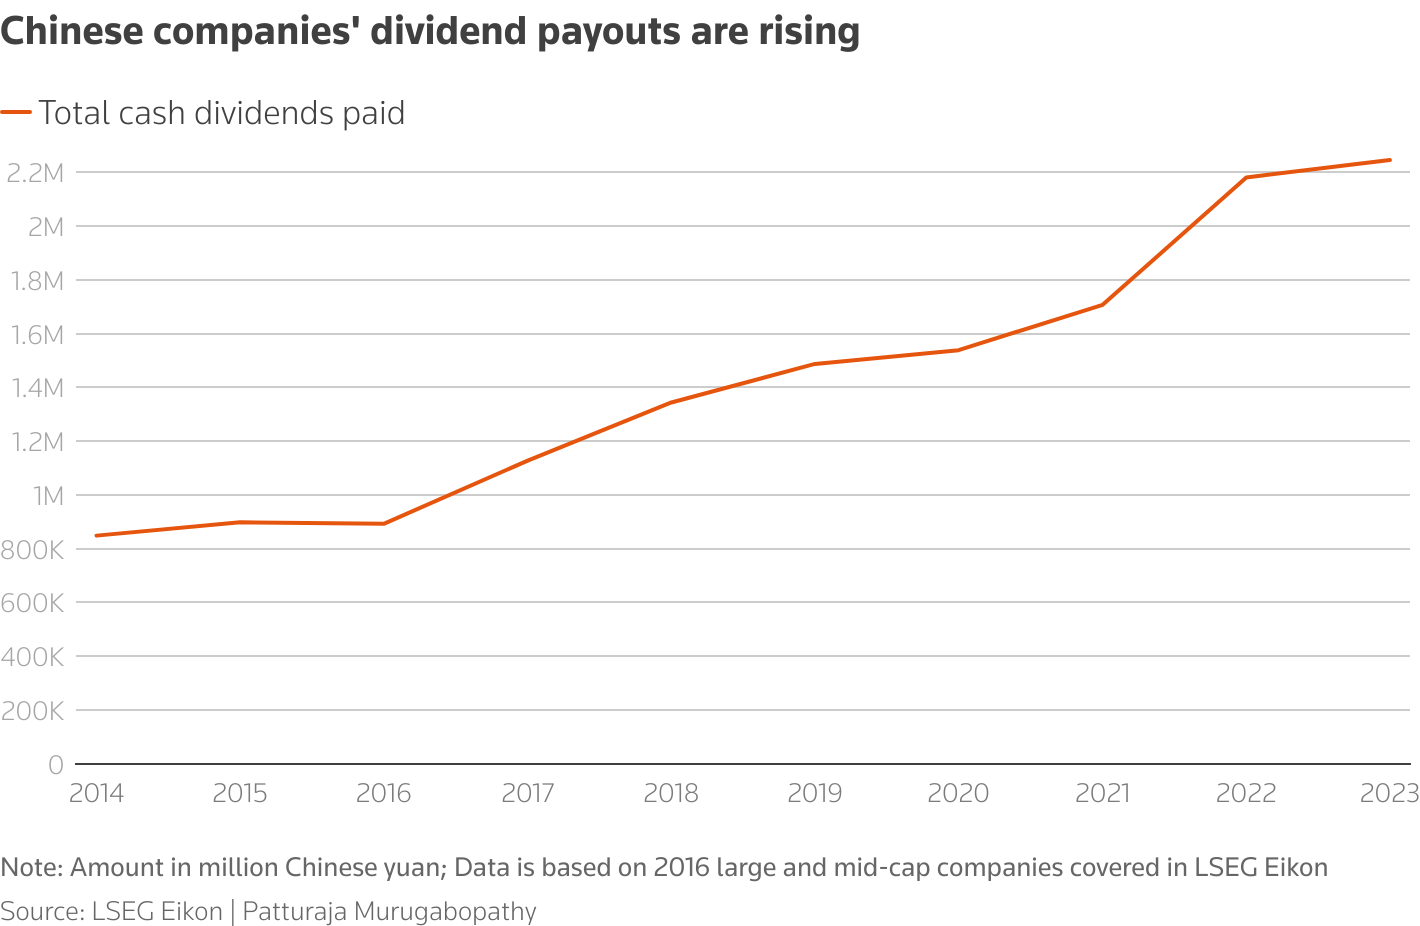
\includegraphics[width=0.75\linewidth]{images/section5/cndprising.png}

\vspace{1mm}
\begin{flushleft}
\scriptsize
\textit{Note:} Data are based on aggregate Chinese-listed companies through approximately 2023. The trend reflects improving cash-return practices; it does not imply all firms are mature dividend payers.
\end{flushleft}
\end{frame}

\begin{frame}{Dividend Payout Ratio: China vs. Other Asian Markets}
\centering
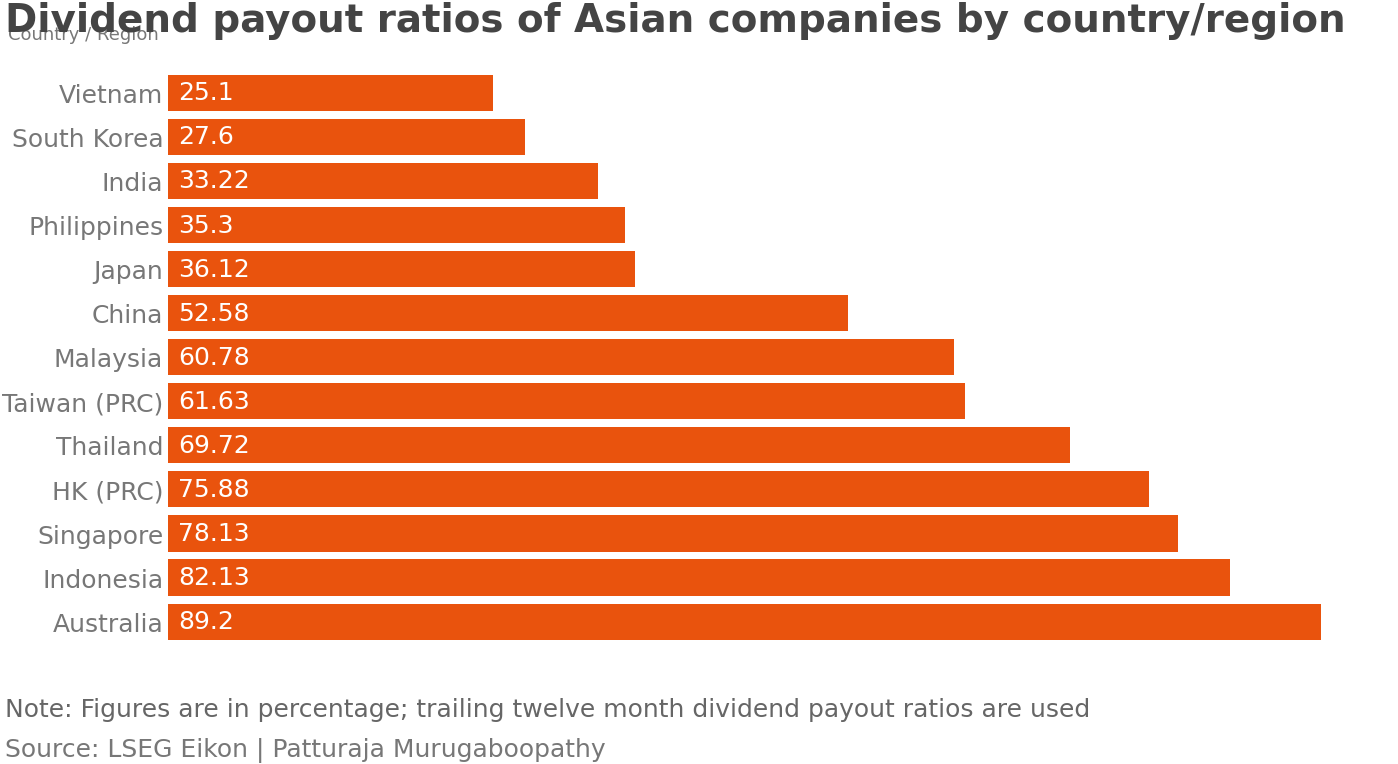
\includegraphics[width=0.65\linewidth]{images/section5/dprbycountry.png}

\vspace{1mm}
\footnotesize
\begin{itemize}
    \item China's payout ratio (52.6\% at end-2023) exceeds Korea, Japan, and India, but trails Singapore, Hong Kong, and Indonesia.
    \item \textbf{Caveat:} Cross-country comparisons reflect differences in industry mix, state ownership, the weight of financial firms, and profitability cycles -- not just payout choices.
    \item Key takeaway: \textbf{China is no longer simply a low-payout market}.
\end{itemize}
\end{frame}

\begin{frame}[t]{China A-Shares: Buybacks Are Rising}
\centering
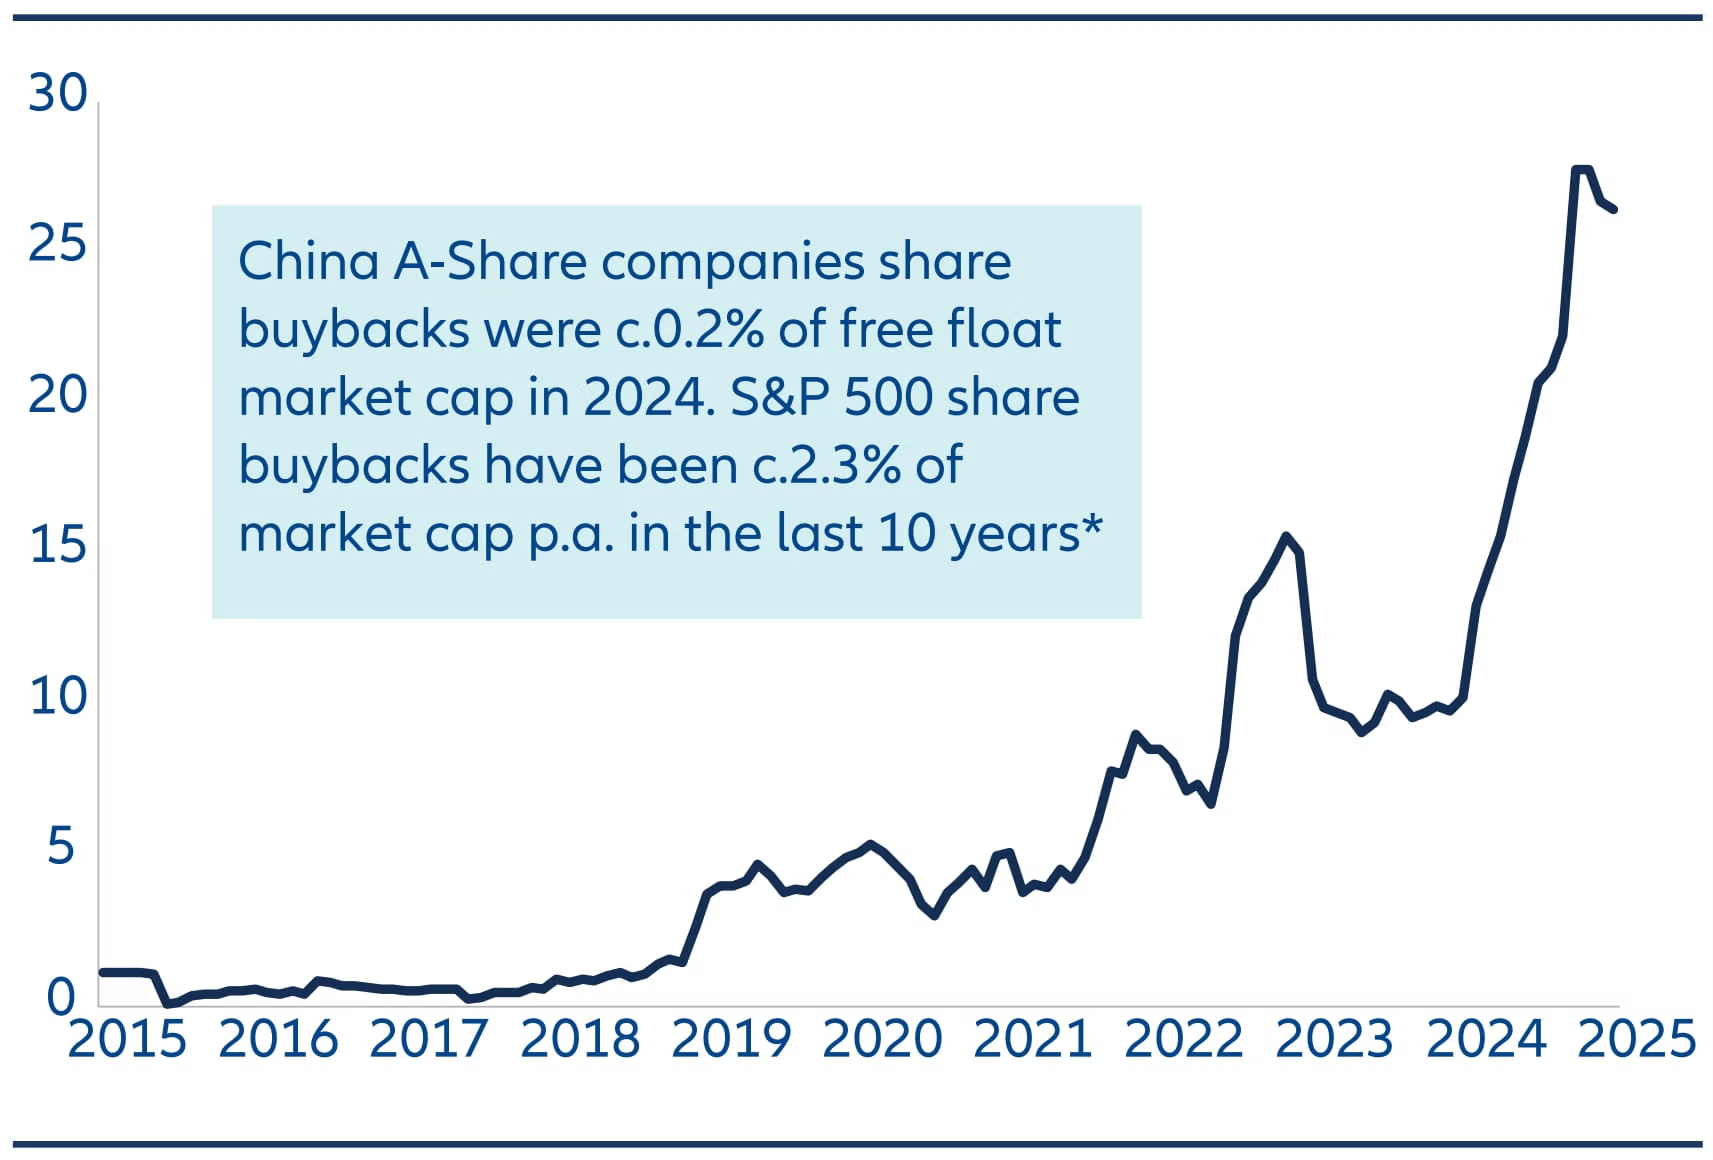
\includegraphics[width=0.68\textwidth]{images/section5/cn_buyback.png}

\vspace{-1mm}
\begin{flushleft}
\footnotesize
\begin{itemize}
    \item Buybacks have become a more visible payout channel in China.
    \item Regulatory encouragement and compressed valuations contributed to the surge in 2024.
\end{itemize}
{\scriptsize Source: Wind / Allianz Global Investors, as of Jan.\ 31, 2025; AllianzGI (2025).}
\end{flushleft}
\end{frame}

\begin{frame}[t]{China Equities: Cash Holdings and Payout Capacity}
\footnotesize
\begin{figure}
    \centering
    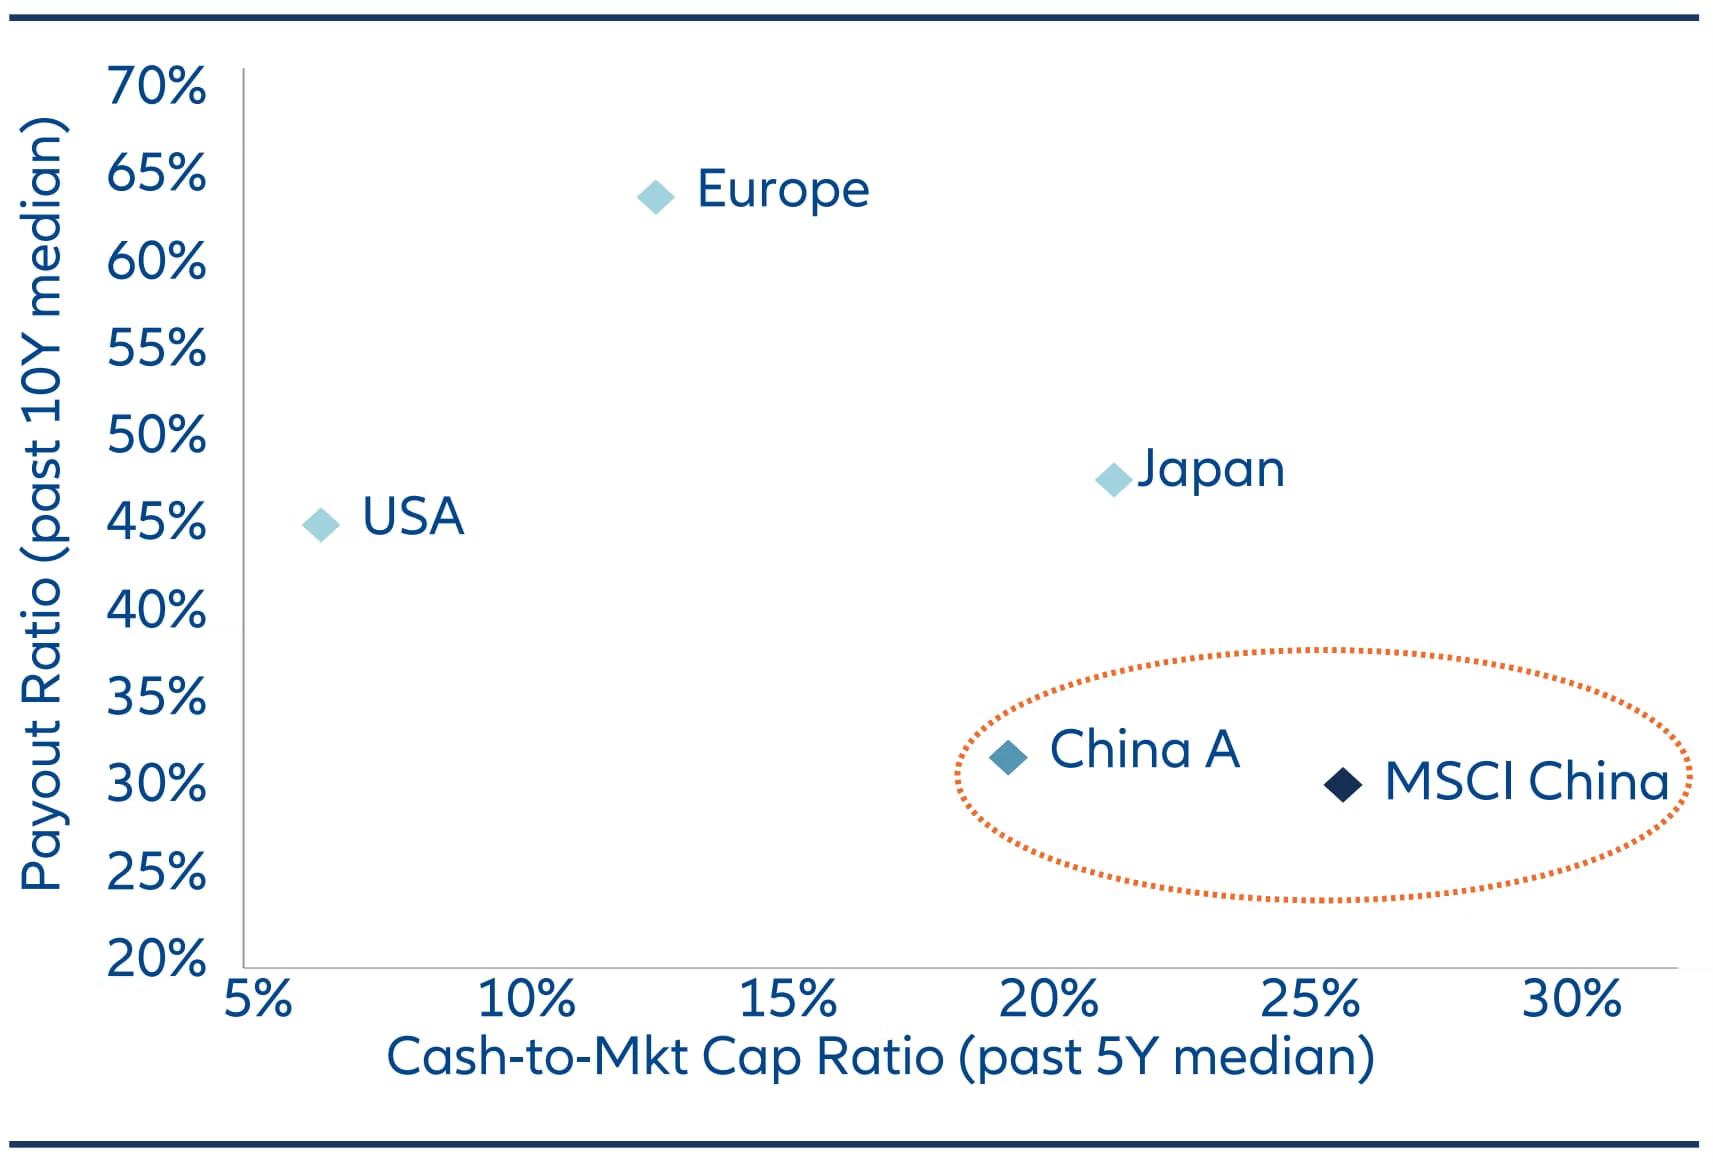
\includegraphics[width=0.62\textwidth]{images/section5/cn_dividend.png}
\end{figure}

\vspace{-0.25cm}

\begin{alertblock}{Interpretation}
Chinese firms hold substantial cash relative to market value, suggesting
room for higher dividends or repurchases. But payout capacity is not the
same as optimal payout.
\end{alertblock}

\vspace{-0.1cm}

{\scriptsize Source: Goldman Sachs, as of Apr.\ 25, 2024; reproduced in AllianzGI (2025).}

\end{frame}

\begin{frame}[t]{Investor Demand: Dividend ETF Inflows}
\footnotesize
\vspace{-0.1cm}
\begin{figure}
    \centering
    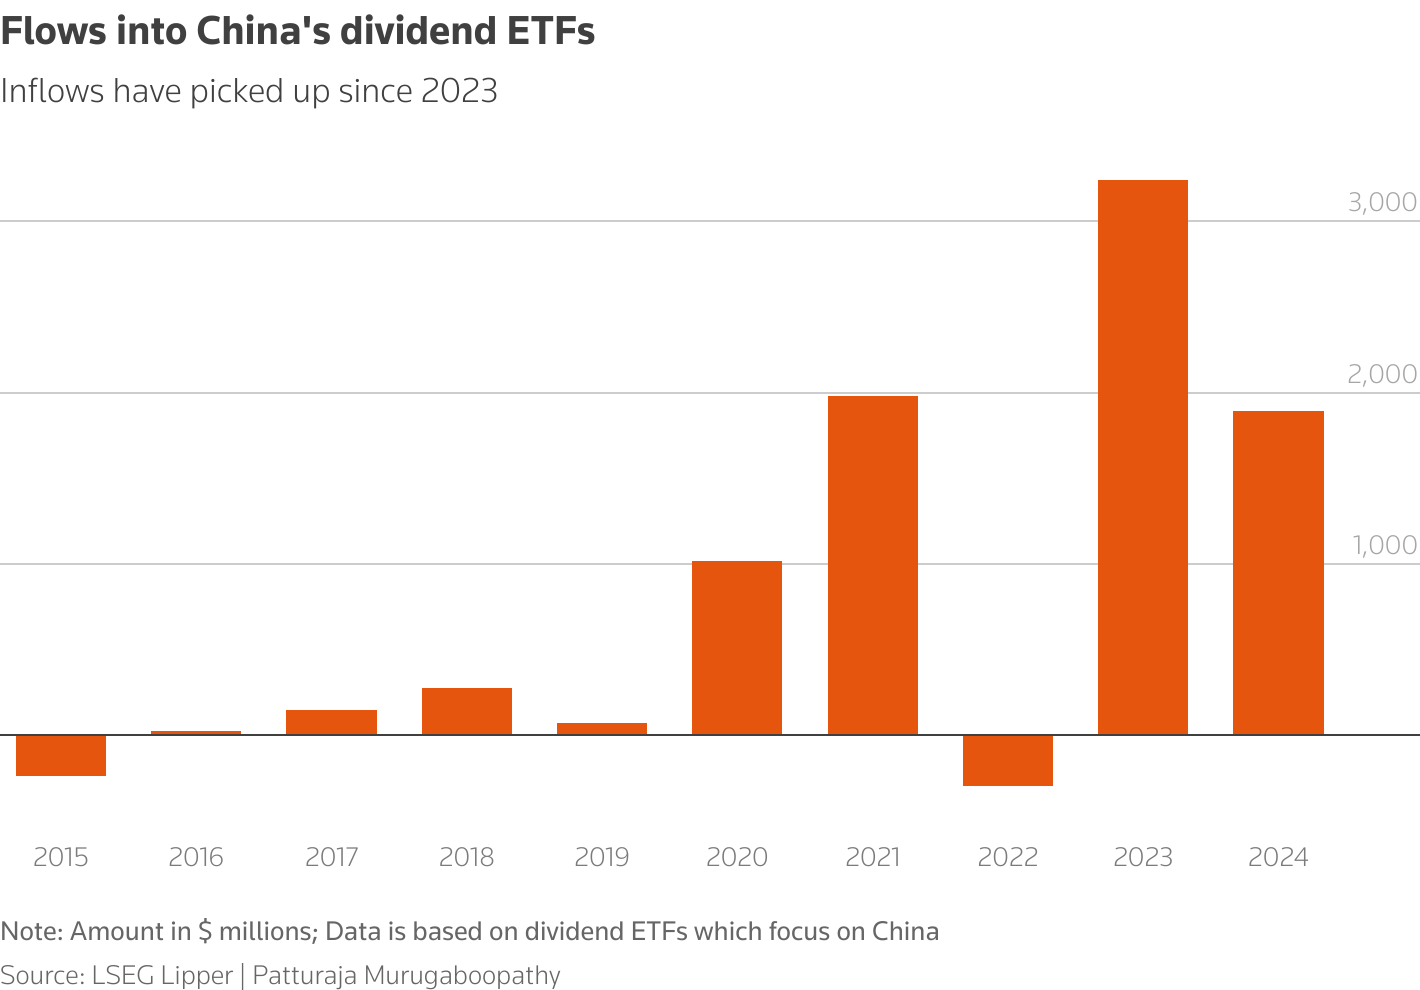
\includegraphics[width=0.64\linewidth]{images/section5/flowintocnde.png}
\end{figure}

\vspace{-0.25cm}

\begin{alertblock}{Interpretation}
Inflows into China dividend ETFs have accelerated since 2020, reflecting
stronger investor demand for cash returns and defensive equity exposure.
\end{alertblock}

{\scriptsize Source: Reuters / LSEG Lipper, based on dividend ETFs mainly focused on China.}

\end{frame}

\begin{frame}{Low Valuations Enhance Dividend Appeal}
\footnotesize
\begin{itemize}
    \item Chinese equities trade at \textasciitilde{}13x forward earnings -- below the S\&P 500 (\textasciitilde{}25x) and Nikkei 225 (\textasciitilde{}15x).
    \item Over 40 Chinese firms have dividend yields higher than their P/E ratios.
    \item Low valuations make dividend and buyback yields more salient; defensive, income-focused strategies gain appeal.
\end{itemize}
\centering
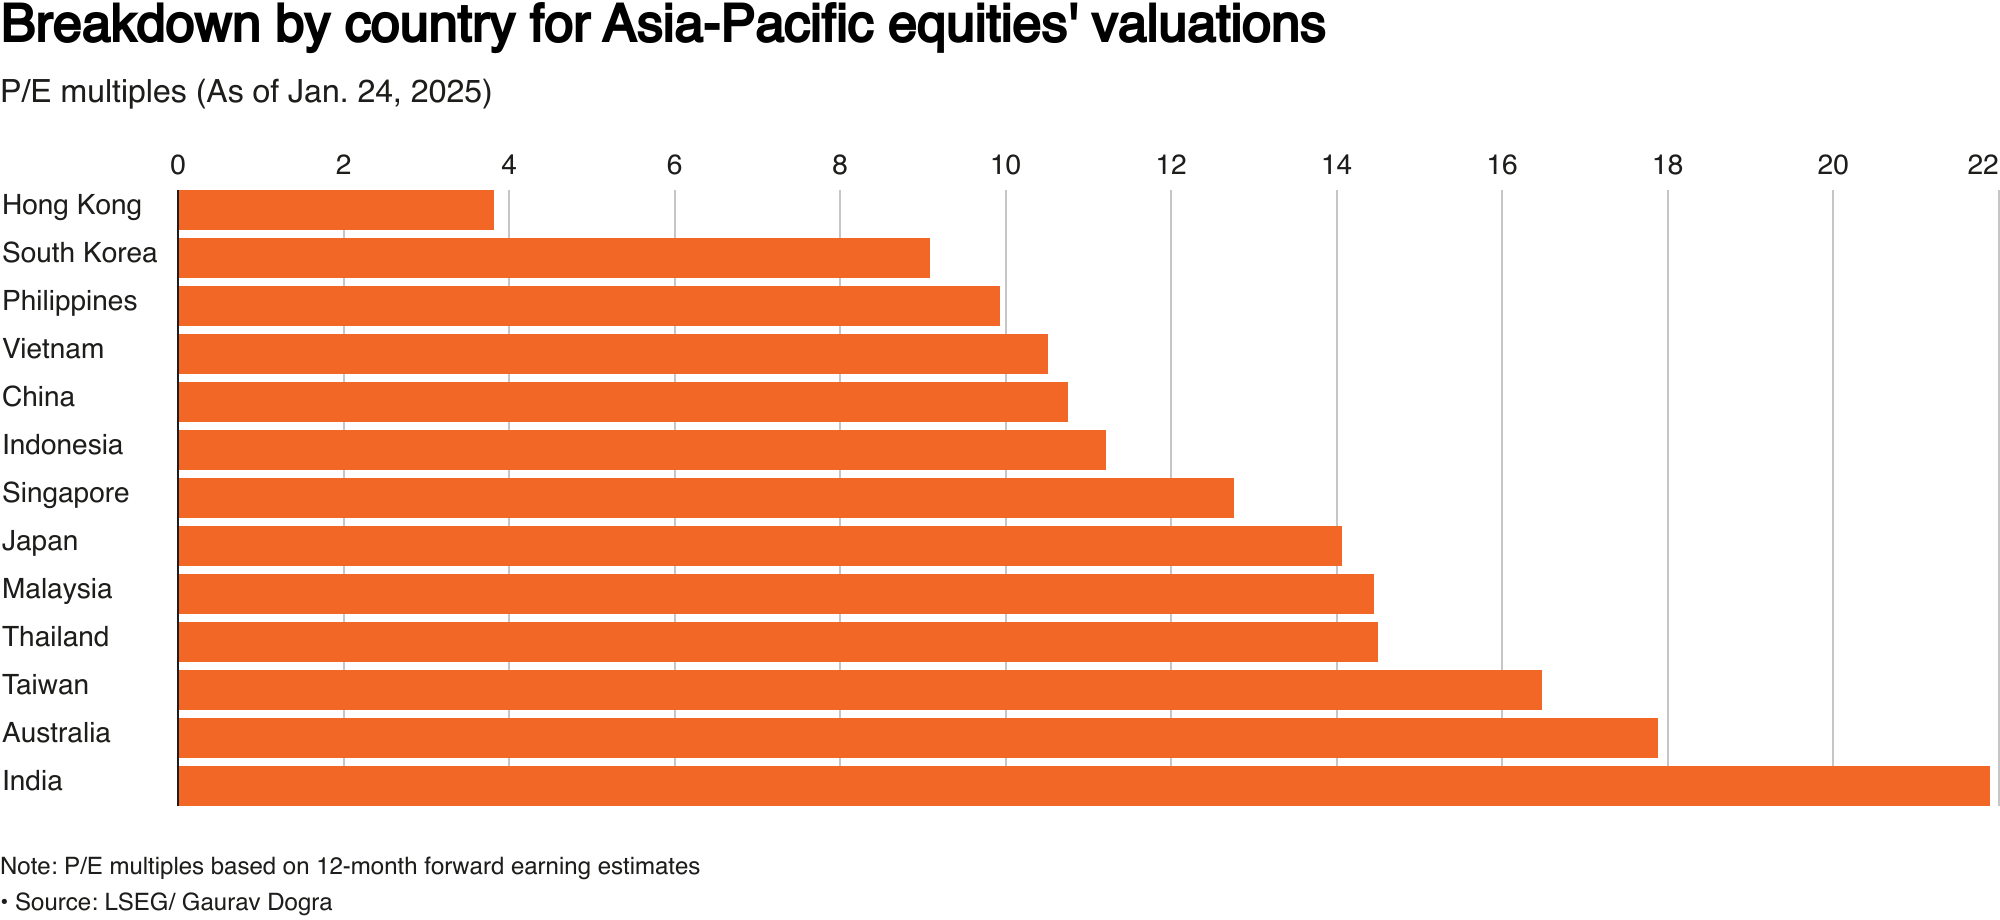
\includegraphics[width=0.85\linewidth]{images/section5/appe.png}
\end{frame}

\begin{frame}{China as a Payout Policy Case}
\footnotesize
\begin{itemize}
    \item \textbf{Governance channel:} Higher payouts reduce idle cash and improve shareholder discipline -- particularly relevant given state ownership and concentrated control.

    \item \textbf{Investor-demand channel:} Dividend ETFs and high-yield strategies attract investors seeking stable cash flows and defensive equity exposure.

    \item \textbf{Valuation channel:} Low valuations make dividend and buyback yields more salient; low prices reinforce the case for returning cash rather than retaining it.

    \item \textbf{Policy channel:} Regulators actively encourage stronger shareholder returns, shaping the institutional environment for rising payouts.
\end{itemize}
\vspace{2mm}
\begin{block}{}
\centering
\textit{China illustrates that payout policy is not only a firm-level decision; it is also shaped by market valuation, investor clientele, and regulatory reform.}
\end{block}
\end{frame}

\subsection{Payout Policy: Synthesis and Managerial Implications}
\begin{frame}{Why Dividends May Matter in Practice}
\footnotesize
\begin{itemize}
    \item \textbf{Investor Demand:} Appeals to income-seeking investors (e.g., retirees) who prefer stable cash flows without selling shares.
    
    \item \textbf{Behavioral Rationale:} Supports self-control -- investors avoid overspending by consuming only dividend income.
    
    \item \textbf{Agency Benefits:}
    \begin{itemize}
        \item Dividends reduce free cash flow available for managerial misuse ("overinvestment" problem).
        \item Limits resources that managers could divert toward empire building or perks.
    \end{itemize}

    \item \textbf{Signaling Value:} Dividend increases can signal management's confidence in future earnings.
\end{itemize}
\end{frame}

\begin{frame}{Costs and Limits of Cash Dividends}
\footnotesize
\begin{itemize}
    \item \textbf{Tax Inefficiency:} Dividends are taxed immediately, while capital gains are taxed only upon realization.

    \item \textbf{Reduced Financial Flexibility:}
    \begin{itemize}
        \item Dividends deplete internal capital.
        \item May force firms to forgo profitable projects or raise costly external equity.
    \end{itemize}

    \item \textbf{Sticky Commitment:} Once initiated, cutting dividends is difficult and often punished by the market.
    
    \item \textbf{Inflexible Tool:} Less adaptable to temporary changes in earnings compared to repurchases.

    \item \textbf{Shareholder--Creditor Conflict:} Large payouts in or near financial distress can transfer value from bondholders to shareholders. This is a value redistribution, not a firm-level benefit of dividends.
\end{itemize}
\end{frame}

\begin{frame}{Dividend Policy: Stylized Facts}
\begin{itemize}
    \item Aggregate corporate payouts (dividends + buybacks) have grown significantly over time.
    \item Dividends are paid primarily by large, mature, and profitable firms.
    \item Managers are reluctant to cut dividends -- they prefer to smooth payments.
    \item Stock prices respond to unexpected dividend changes (positive or negative).
    \item Repurchases are more volatile -- often tied to temporary earnings or stock price fluctuations.
\end{itemize}
\end{frame}

\begin{frame}{Managerial Guidelines for Payout Policy}

\begin{itemize}
    \item \textbf{Investment first:}
    Do not sacrifice positive-NPV projects to maintain or increase payouts.

    \item \textbf{Base regular dividends on sustainable cash flows:}
    Initiate dividends only when free cash flow is stable and predictable.

    \item \textbf{Smooth dividends:}
    Adjust regular dividends gradually, consistent with long-run earnings capacity.

    \item \textbf{Use repurchases for flexibility:}
    Buybacks are better suited for temporary excess cash or perceived undervaluation.

    \item \textbf{Consider taxes, clientele, and governance:}
    The optimal payout policy depends on investor preferences, tax treatment,
    agency problems, and financing constraints.
\end{itemize}

\vfill

\begin{alertblock}{Takeaway}
Payout policy should distribute excess cash without weakening investment
capacity, financial flexibility, or long-term firm value.
\end{alertblock}

\end{frame}

\subsection{Non-Cash Payouts: Stock Dividends and Stock Splits}

\begin{frame}{Non-Cash Payouts and Share Count Adjustments}
\begin{itemize}
    \item \textbf{Cash dividends:} Transfer cash from the firm to shareholders; firm value falls by the amount distributed.

    \item \textbf{Stock dividends:} Distribute additional shares to existing shareholders. No cash leaves the firm.

    \item \textbf{Stock splits:} Increase the number of shares and mechanically reduce price per share (e.g., a 2-for-1 split doubles share count and halves price).

    \item \textbf{Reverse splits:} Reduce the number of shares and mechanically increase price per share (e.g., a 1-for-10 reverse split).
\end{itemize}

\vspace{3mm}
\begin{block}{Key Idea}
Stock dividends, splits, and reverse splits change share count and per-share figures, but do \textbf{not} directly change total firm value.
\end{block}
\end{frame}

\begin{frame}{Peterson Co.: Stock Dividend Example}
\small
\textbf{Setup:} Peterson Co.\ declares a \textbf{10\% stock dividend}. Initial position: 10,000 shares at \$66/share (market cap \$660,000).

\vspace{3mm}
\begin{center}
\begin{tabular}{lccc}
\toprule
 & \textbf{Before} & \textbf{After} & \textbf{Change} \\
\midrule
Shares outstanding & 10,000 & 11,000 & $+$1,000 \\
Price per share & \$66.00 & \$60.00 & $-\$6.00$ \\
Market capitalization & \$660,000 & \$660,000 & None \\
\bottomrule
\end{tabular}
\end{center}

\vspace{2mm}
{\footnotesize Theoretical ex-price: $\$66 \times \frac{10{,}000}{11{,}000} \approx \$60.00$}

\vspace{2mm}
\begin{itemize}
    \item Total market value is mechanically unchanged.
    \item Each shareholder holds more shares, but each share is worth proportionally less.
    \item Proportional ownership is unchanged; no cash is distributed.
    \item \textit{Accounting note:} retained earnings are reclassified into paid-in capital --- no net equity change.
\end{itemize}
\end{frame}

\begin{frame}{Why Do Firms Split Shares?}
\begin{itemize}
    \item \textbf{Trading range:} Stocks priced too high may deter small investors. Splits keep the price in a psychologically or institutionally favorable range.

    \item \textbf{Perceived affordability:} A lower nominal price can attract retail investors and improve marketability.

    \item \textbf{Liquidity:} More shares at a lower price may improve bid-ask spreads and trading activity.

    \item \textbf{Reverse splits:} Used to avoid exchange delisting (e.g., Nasdaq's \$1 minimum price rule) or to eliminate administratively small shareholdings.
\end{itemize}

\vspace{3mm}
\begin{alertblock}{Caveat}
Splits are mostly cosmetic in valuation terms. Any lasting valuation effect must come from liquidity, signaling, or investor perception --- not from mechanical share-count changes.
\end{alertblock}
\end{frame}

\begin{frame}[t]{Stock Split vs.\ Large Stock Dividend}
\small
\begin{center}
\begin{tabular}{@{} l >{\raggedright\arraybackslash}p{3.6cm} >{\raggedright\arraybackslash}p{3.6cm} @{}}
\toprule
 & \textbf{Stock Split} & \textbf{Large Stock Dividend ($\geq 20\%$)} \\
\midrule
Share count      & Increases (e.g., $2\times$)  & Increases (e.g., $2\times$)  \\[2pt]
Price per share  & Falls proportionally          & Falls proportionally          \\[2pt]
Cash flow        & None                          & None                          \\[2pt]
Accounting       & Par value per share reduced; retained earnings unchanged & Retained earnings reclassified to paid-in capital (at par value) \\[2pt]
Total firm value & Unchanged                     & Unchanged                     \\
\bottomrule
\end{tabular}
\end{center}

\vspace{3mm}
\footnotesize \textbf{Example:} A 100\% stock dividend (one new share issued per share held) and a 2-for-1 split are economically equivalent --- the difference lies only in accounting treatment.
\end{frame}

\begin{frame}{Stock Dividends and Splits: Main Takeaway}
\begin{block}{}
\centering
Stock dividends and stock splits change the number of shares outstanding, but do \textbf{not} directly change total firm value.
\end{block}

\vspace{3mm}
\begin{itemize}
    \item \textbf{Cash dividends:} Distribute cash to shareholders; firm value falls.
    \item \textbf{Stock dividends:} Distribute shares; no cash leaves the firm.
    \item \textbf{Stock splits:} Mechanically lower price per share by increasing share count.
    \item \textbf{Reverse splits:} Mechanically raise price per share by reducing share count.
\end{itemize}

\vspace{3mm}
\begin{alertblock}{Practical Relevance}
These actions are mostly cosmetic in valuation terms, but they may matter for \textbf{liquidity}, \textbf{investor perception}, and \textbf{exchange listing requirements}.
\end{alertblock}
\end{frame}

\subsection*{Summary}
\begin{frame}{Summary: Dividends and Other Payouts}
\footnotesize
\begin{itemize}
  \item \textbf{Dividend Irrelevance (Theory)}: In perfect markets, payout policy does not affect firm value. Investors can create "homemade dividends."
  \item \textbf{Practical Frictions}:
  \begin{itemize}
    \item Taxes: Dividends are often taxed more heavily than capital gains.
    \item Agency issues: Dividends reduce managerial discretion over cash.
    \item Signaling: Dividend changes convey management's private information.
  \end{itemize}
  \item \textbf{Real-World Payout Practices}:
  \begin{itemize}
    \item Firms prefer to smooth dividends and avoid cuts.
    \item Share repurchases are more flexible and tax-efficient, increasingly favored.
    \item Payout decisions reflect investor preferences, corporate governance, and market norms.
  \end{itemize}
  \item \textbf{Stock Dividends and Splits}:
  \begin{itemize}
    \item Stock dividends and splits do not change total firm value.
    \item Often used to keep stock price in a desirable trading range or meet listing requirements.
  \end{itemize}
\end{itemize}
\end{frame}


\begin{frame}
	\Huge{\centerline{The End}}
\end{frame}
\backupbegin

\section*{Reference}
\begin{frame}[allowframebreaks]{References}
	\printbibliography[heading=none]
\end{frame}

\backupend

%----------------------------------------------------------------------------------------

\end{document}